% This template was written by John Davies <john.davies@glasgow.ac.uk> 2017-02-06
% It matches the university specification at the time of writing
%   for the widths of the page margins and one-and-a-half line spacing
% You may want to include more packages, particularly for heavy mathematics
% Please let me know if you find any errors or wish to suggest improvements

\documentclass[12pt,titlepage,oneside]{book}
\usepackage[T1]{fontenc} % modern encoding
% Comment out the next three lines of LaTeX if you wish to use Computer Modern fonts
%   (this is the default for LaTeX)
% Make sure that your TeX installation can produce good pdf with these fonts.
% The following three lines are a good alternative if you don't use much mathematics
\usepackage{mathptmx}  % uses Times for text and mathematics
\usepackage[scaled]{helvet} %  helvetica for sanserif, scaled 95% by default
\usepackage{courier}  % courier for typewriter font, pretty ugly but available
% otherwise the stix package offers more options and symbols
% \usepackage{stix}  % uses Times for text and a range of fonts for mathematics
% End of choices for fonts
\usepackage{graphicx}  % standard package for importing graphics files
\usepackage{cite}  % improves format of numerical citations, such as [1-3]
\usepackage[top=1.8cm, bottom=1.8cm,left=4.0cm,right=1.5cm]{geometry}
% These margins are the university guidelines
%\usepackage[onehalfspacing]{setspace}  % gives one-and-a-half line spacing
% doublespacing is another option and can be changed in the text
\usepackage[doublespacing]{setspace}
\usepackage{dcolumn}% Align table columns on decimal point
\usepackage{bm}% bold math
\usepackage{amsmath}
\usepackage{amsfonts}
\usepackage{amssymb}
\usepackage{color}
\usepackage{acronym}
\usepackage{multirow}
\usepackage{tabularx}
\usepackage{hyperref}

\hypersetup{
%--- fill inside borders ---
  colorlinks=true,        % false: boxed links; true: colored links
  linkcolor=black,         % color of internal links
  citecolor=cyan,         % color of links to bibliography
}

%% ----- comment commands for each of us
\newcommand{\chris}[1]{\textbf{\textcolor{red}{CHRIS: #1}}}
\newcommand{\francesco}[1]{\textbf{\textcolor{green}{FRANCESCO: #1}}}
\newcommand{\hunter}[1]{\textbf{\textcolor{blue}{HUNTER: #1}}}
\newcommand{\siong}[1]{\textbf{\textcolor{cyan}{SIONG: #1}}}
\newcommand{\rod}[1]{\textbf{\textcolor{yellow}{ROD: #1}}}

\acrodef{GW}[GW]{Gravitational wave}
\acrodef{BBH}[BBH]{binary black hole}
\acrodef{CW}[CW]{continuous gravitational waves}
\acrodef{EM}[EM]{electromagnetic}
\acrodef{CBC}[CBC]{compact binary coalescence}
\acrodef{BNS}[BNS]{binary neutron star}
\acrodef{NSBH}[NSBH]{neutron star black hole}
\acrodef{PSD}[PSD]{power spectral density}
\acrodef{ELBO}[ELBO]{evidence lower bound}
\acrodef{LIGO}[LIGO]{advanced Laser Interferometer Gravitational wave Observatory}
\acrodef{LISA}[LISA]{Laser Interferometer Space Antenna}
\acrodef{CVAE}[CVAE]{conditional variational autoencoder}
\acrodef{KL}[KL]{Kullback--Leibler}
\acrodef{GPU}[GPU]{graphics processing unit}
\acrodef{LVC}[LVC]{LIGO-Virgo Collaboration}
\acrodef{PP}[p-p]{probability-probability}
\acrodef{SNR}[SNR]{signal-to-noise ratio}
\acrodef{AE}[AE]{autoencoder}
\acrodef{VAE}[VAE]{variational autoencoder}
\acrodef{LSTM}[LSTM]{Long Short Term Memory}
\acrodef{GR}[GR]{general relativity}

\acrodef{FFT}[FFT]{fast Fourier transform}
\acrodef{CNN}[CNN]{convolutional neural network}
\acrodef{ROC}[ROC]{receiver operator characteristic}
\acrodef{MCMC}[MCMC]{Markov Chain Monte Carlo}
\acrodef{ML}[ML]{machine learning}
\acrodef{ANN}[ANN]{artificial neural network}
\acrodef{MAF}[MAF]{masked autoregressive flow}
\acrodef{GAN}[GAN]{generative adversarial network}
\acrodef{RF}[RF]{random forest}
\acrodef{GP}[GP]{genetic programming}


\begin{document}
\begin{titlepage}
\centering
\vspace*{3cm}  % Need the * or the space is swallowed at the top of the page
\bfseries\Large
Optimizing the search for Gravitational Waves using Machine Learning \\
\vspace{3cm}
\normalfont\large
Hunter Gabbard\\
\vspace{2cm}
Submitted in fulfilment of the requirements for the\\
Degree of Doctor of Philosophy\\
\vspace{2cm}
School of Physics and Astronomy\\
College of Science and Engineering\\
University of Glasgow\\
\vspace{1cm}
\includegraphics[scale=0.125]{GlaLogo.pdf}
\\
\vspace{1cm}
% Insert month and year of date deposited with library for final version
October 2021
\end{titlepage}
\frontmatter  % Turn off chapter numbering, use roman page numbers
\chapter{Abstract}

Over 100 years ago Einstein formulated his now famous theory of 
General Relativity. In his theory he lays out a set of equations 
which lead to the beginning of a brand-new 
astronomical field, \ac{GW} astronomy. The \ac{LVK}'s
aim is the detection of \ac{GW} events from some of the most violent 
and cataclysmic events 
in the known universe. The \ac{LVK} detectors are composed of 
large-scale Michelson Morley interferometers which are able to detect 
\acp{GW} from a range 
of sources including: \acp{BBH}, \acp{BNS}, 
\acp{NSBH}, supernovae and stochastic \acp{GW}. 
Although these \ac{GW} events release an incredible amount of 
energy, the amplitudes of the \acp{GW} from such events 
are also incredibly small. 

The \ac{LVK} uses sophisticated techniques such as matched 
filtering and Bayesian inference in order 
to both detect and infer source parameters 
from \ac{GW} events. Although optimal under many 
circumstances, these standard methods are computationally 
expensive to use. Given the expected of order $100$s of \ac{GW} 
signals the detectors are expecting to see in the coming years, there 
is an urgent need for less computationally expensive detection and 
parameter inference techniques. A possible solution to reducing the computational 
expense of such techniques is the exciting field of \ac{ML}.

%
% Matched filtering
%
In this thesis, we deploy 
various \ac{ML} and statistical techniques such as 
\acp{CVAE} and \acp{CNN} in two first-of-their-kind proof-of-principle 
studies. We describe how we used 
a \ac{CNN} which can match the sensitivity of matched 
filtering, the standard technique used by the \ac{LVK} 
for detecting \acp{GW}. We show how our \ac{CNN} may be trained using 
simulated \ac{BBH} waveforms buried in Gaussian noise 
and signals with Gaussian noise alone. We compare the results 
of our \ac{CNN} classification predictions to results from 
matched filtering given the same testing data as the 
\ac{CNN}. In our results we are able to show using receiver 
operating charactersitics and efficiency curves that our \ac{ML} approach 
is able to generally achieve the same levels of sensitivity as that of 
matched filtering. It is also shown that the \ac{CNN} approach is 
able to generate predictions in low-latency. Given approximately $25000$ test cases,  
the \ac{CNN} is able to produce classification predictions for all in $\mathds{1}$s.

%
% ML for Bayesian inference
%
In our second study, we show how \acp{CVAE} may be used in order 
to perform Bayesian inference. We train our \ac{CVAE} using simulated 
\ac{BBH} waveforms in Gaussian noise, as well as the source parameter 
values of those waveforms. When testing, the \ac{CVAE} is only supplied 
the \ac{BBH} waveform and is able to produce samples from the 
Bayesian posterior. We compare our results to that of several standard 
Bayesian samplers used by the \ac{LVK} including: \texttt{Dynesty}, 
\texttt{ptemcee}, \texttt{emcee}, and \texttt{CPnest}. It is shown that 
when properly trained our \ac{CVAE} method is able to produce Bayesian 
posteriors which are generally consistent with other Bayesian samplers. Our results 
are quantified using a variety of figures of merit such as \ac{PP} plots 
in order to check the 1-dimensional marginalised posteriors from all 
approaches are self-consistent with the frequentist perspective. We also 
employ the use of the \ac{JS}-divergence in order to compute the similarity 
of different posterior distributions from one another, as well as other 
figures of merit explained later in this thesis. We also demonstrate that our 
\ac{CVAE} model is able to produce posteriors with $8000$ samples in under 
a second, representing a $6$ order of magnitude increase in performance 
over traditional sampling methods. 


\tableofcontents
\listoftables
\listoffigures
\chapter{Acknowledgements}

I would first off like to thank my parents (Lisa Gabbard and Kurt Gabbard) for all that they've done for me. Without their constant encouragement growing up and to the present day I would not be where I am now. Additionally, I would like to thank the rest of my family including my siblings (Mallory and Schuyler), my grandfather (Evan Lewis). 

To the many advisors that I've had over my short research career including: Prof. Marco Cavaglia, Dr. Florent Robinet, Dr. Soma Mukherjee, Dr. Andrew Lundgren, Prof. Ik Siong Heng and Dr. Chris Messenger.

\chapter{Declaration}

With the exception of chapters \ref{ch:chap_1}, \ref{ch:chap_2} and \ref{ch:chap_3}, which contain introductory material, 
all work in this thesis was primarily carried out by the author under the supervision
of Prof. Ik Siong Heng and Dr. Chris Messenger unless otherwise explicitly stated. 

The work carried out in Ch.~\ref{ch:chap_4}, was primarily 
done by myself under the supervision of Dr. Chris Messenger 
and Prof. Ik Siong Heng, along with support from co-authors 
Mr. Fergus Hayes and Mr. Michael Williams. Both Michael Williams 
and Fergus Hayes had carried out initial studies and produced some 
intial code to work from. Michael Williams, along with myself, 
produced the machine learning code used in the analysis. I, along with input from 
Chris Messenger, produced the matched filtering code used in the 
analysis. All co-authors 
on the published paper version of this analysis~\cite{PhysRevLett.120.141103} 
have also contributed to the text of the published manuscript. 
Both Chris Messenger and Ik Siong Heng provided advice 
on the thesis chapter version of the published manuscript.

The work carried out in Ch.~\ref{ch:chap_5} was primarily 
lead by myself under the supervision of Dr. Chris Messenger 
and Prof. Ik Siong Heng, along with support from co-authors 
Mr. Francesco Tonolini and Prof. Roderick Murray-Smith. Both 
Francesco Tonolini and Roderick Murray-Smith provided guidance 
on the machine learning methods used, some initial machine learning code to work from, 
as well as input 
on the text released in the public version of the manuscript
found here~\cite{1909.06296}. Chris Messenger and Ik Siong Heng also provided 
input to the text in the public form of the manuscript, as well as advice on 
the thesis chapter version.

The final conclusions chapter (Ch.~\ref{ch:chap_6}) was written by myself, with advice 
from Chris Messenger and Ik Siong Heng.


\mainmatter % Turn on chapter numbering, reset page numbers, use arabic
\chapter[Introduction to Gravitational waves]{An Introduction to Gravitational Waves, Search Methods and Parameter Estimation Techniques}\label{ch:chap_1}

\hunter{Hey Chris. This chapter is ready for you to review again. I will 
note that I did try to move the GW detection section to the beginning 
of the chapter, but I think there are just too many concepts in there 
that need to be explained first for that to work, so I've left it at the 
end of the chapter.}

\section{General Relativity and Gravitational Waves}

Gravitational waves were predicted by Einstein in his theory of \ac{GR}
well over 100 years ago \cite{GR_Einstein_paper}. In his theory, Einstein 
shows that the more massive an object is, the more curvature in spacetime that object creates. This curvature then has an effect on the motion of objects which encounter it. This effect is summarized succinctly by John 
Archibald Wheeler where he states that ``Spacetime tells matter how to move; matter tells spacetime how to curve''. Curvature may be quantified by first defining a term known as the Riemann curvature 
tensor $R^{\rho}_{\sigma\mu\nu}$. The Riemann tensor describes the change 
experienced by a vector which has been parallel transported over a curved 
manifold\cite{carroll_2019}. Einstein formalises the relationship between matter/energy and the curvature of space-time in his field equations as
%
\begin{equation}\label{eq:FieldEquations}
    G_{\mu \nu} + \Lambda g_{\mu \nu} = \frac{8 \pi G}{c^{4}} T_{\mu \nu},
\end{equation}{}
%
where $\Lambda$ is the cosmological constant (scalar measurement describing the energy density of space), $g_{\mu \nu}$ is the metric which describes the geometric structure of space-time, $G$ is Newton's gravitational constant, $c$ is the speed of light, $T_{\mu \nu}$ is the stress energy tensor which describes the density, direction, and flow of energy in space-time. $G_{\mu \nu}$ is the Einstein tensor defined as
%
\begin{equation}
    G_{\mu \nu} = R_{\mu \nu} - \frac{1}{2} R g_{\mu \nu}
\end{equation}
%
where $R_{\mu \nu}$ is the Ricci curvature tensor (a contraction of the Riemann 
curvature tensor) and $R$ is the Ricci scalar defined as the trace 
of the Ricci curvature tensor. 

%
% Transition towards discussing GWs as small purturbations on the flat spacetime metric
%
The Einstein field equations described by Eq.~\ref{eq:FieldEquations} can  unfortunately only be solved exactly analytically in a limited number of situations. Some solutions include the Schwarzschild solution for a non-spinning singularity (where a singularity is defined as a point in spacetime where 
there is predicted to be infinite curvature~\cite{carroll_2019}) and the Kerr solution for a spinning singularity. 

In the regime of small perturbations 
to spacetime, considering we would like to explore the behavior of non-linear, time-dependent systems in terms of Einstein's field equations, 
we need to put his equations into a more linear form. This can be done by describing the spacetime metric $g_{\mu\nu}$ in terms of an easily computable known solution in flat spacetime with the addition of some small perturbation,
%
% Introduce g_munu
%
where \ac{GW}s may be defined as small perturbations over the curved background spacetime metric $g_{\mu \nu}$. In Euclidean space, the metric (which is what allows us to compute distances or dot products between two point mass objects), is generally described by the identity matrix in Cartesian coordinates. However, in \ac{GR} we have to add the time dimension and in flat spacetime this can be described by the Minkowski metric tensor $\bar{g}_{\mu \nu}$ (sometimes also denoted $\eta_{\mu \nu}$) given by 
%
\begin{equation}
  \bar{g}_{\mu \nu} =   \begin{pmatrix}
-1 & 0 & 0 & 0\\
0 & 1 & 0 & 0\\
0 & 0 & 1 & 0\\
0 & 0 & 0 & 1
\end{pmatrix},
\end{equation}
%
where each column and row represent a dimension of spacetime 
(from left to right and top to bottom: $ct,x,y,z$) where $t$ denotes time, $c$ is the speed of light, 
and $x,y,z$ denote the 
3 spacial dimensions. Time $t$ is negative because the speed 
of light $c$ must remain constant when changing between frames of 
reference \cite{carroll_2019} \hunter{Need Chris to check this}. 
Although the Minkowski metric can be written in non-diagonal 
forms depending on choice of coordinates, this diagonal form 
is chosen because it is computationally easy to invert 
and simple to compute the determinant of the matrix.

Since a \ac{GW} is a perturbation, we can write the metric tensor 
of a small perturbation in flat spacetime as 
%
\begin{equation}
    g_{\mu \nu} = \bar{g}_{\mu \nu} + h_{\mu \nu},
\end{equation}{}
%
where $h_{\mu \nu}(x)$ is the \ac{GW} perturbation tensor ($|h_{\mu \nu}(x) \ll 1|$). 
%Taking the derivative of the metric tensor we arrive at 
%the wave equations, 
%
%\begin{equation}\label{eq:wave_eq}
%    \Box\bar{h}_{\mu\nu} \equiv \Box\bar{h}_{\mu\nu,\alpha}^{\alpha} = 0 
%\end{equation}
%
%where $\Box$ is the  d'Alembertian operator and $\bar{h}_{\mu\nu}$ is 
%a rescaling of the \ac{GW} perturbation tensor in order 
%to simplify Eq.\ref{eq:wave_eq} and may be defined as 
%
%\begin{equation}
% \bar{h}_{\mu\nu} = h_{\mu\nu} - \frac{1}{2}\eta_{\mu\nu}h   
%\end{equation}
%
%One of the well-known solutions to Eq. \ref{eq:wave_eq} is  
%given as 
%
%\begin{equation}\label{eq:gw_plane_solution}
%    h_{\mu\nu} = \textrm{Re}[A_{\mu\nu} e^{ik_{\alpha}x^{\alpha}}],
%\end{equation}{}
%
%where $A_{\mu\nu}$ is the amplitude tensor, $k_{\alpha}$ is the covariant %wavevector and $x^{\alpha}$ is 
%position in spacetime.
%This is also known as the plane wave solution. 
\ac{GW} perturbations are themselves generated by 
accelerating masses which produce 
higher order quadrupole (or multipole) moments~\cite{Maggiore:2007ulw}.

Using $g_{\mu\nu}$, we find that one of the solutions to the linearised 
form of Einstein's field equations may be written as a plane-wave 
solution given by
%
\begin{equation}\label{eq:gw_plane_solution}
    h_{\mu\nu} = \textrm{Re}[A_{\mu\nu} e^{ik_{\alpha}x^{\alpha}}],
\end{equation}{}
%
where $A_{\mu\nu}$ is a complicated amplitude tensor made up 
of multiple independent components and $h_{\mu \nu}$ is a sinusoidal 
wave traveling along the null wavevector $k$~\cite{Maggiore:2007ulw}.

Exploiting guage freedoms~\cite{carroll_2019}, we 
can shift to the Transverse Traceless 
gauge (since this simplifies the plane-wave solution of Einstein's field 
equations to a simplified metric which is only made up of two 
unique components) 
%(since it is convenient to do 
%so given that the metric perturbation is perpendicular to the 
%wavevector in this guage~\cite{Sathyaprakash2009}) 
and $h_{\mu \nu}$ can be rewritten as
%
\begin{equation}
  h_{\mu \nu} =   \begin{pmatrix}
0 & 0 & 0 & 0\\
0 & h_{+} & h_{\times} & 0\\
0 & h_{\times} & -h_{+} & 0\\
0 & 0 & 0 & 0
\end{pmatrix}.
\end{equation}
%
where $h_{+}$ and $h_{\times}$ are representative of the two 
polarization states of a \ac{GW} which are orthogonal to 
one-another~\cite{carroll_2019,Anderson2011}.

%
% h+ and h_cross from a binary system.
%
As derived in~\cite{Capano2011SearchingFG}, assuming that the 
source of the \ac{GW} is emitted from 
a binary astrophysical system with component masses $m_1,m_2$, 
the plus and cross polarization states can 
be expressed as being equivalent to
%
\begin{align}
    h_{+} &\equiv \frac{1}{d} (1 + \mathrm{cos}^{2}\iota) 2\mu(M\Omega^{2/3})
    \mathrm{cos}(2(\Omega t - \phi_0))
    \\
    h_{\times} &\equiv \frac{1}{d} \mathrm{cos}\iota 2\mu(M\Omega^{2/3})
    \mathrm{sin}(2(\Omega t - \phi_0))
\end{align}
%
where $d$ is the distance to the source, $\iota$ is the inclination 
angle of the binary with respect to an observer, $M$ is the total 
mass of the system, $\phi_0$ is the initial phase of the system,  
$t$ is time, $\mu$ is the reduced mass given as $\frac{m_1 m_2}{M}$
and $\Omega$ is Kepler's third law given by
%
\begin{equation}
    \Omega = \sqrt{\frac{M}{a^3}}
\end{equation}
%
where $a$ is the seperation distance between the two component 
masses of the system.

The effect that a passing 
\ac{GW} waveform has on a set of freely floating test particles as 
a function of the waveform's phase $\phi$ for a given polarization state is 
illustrated in Fig. \ref{fig:gw_plus_cross}. This effect on freely floating test masses is what is measured by \ac{LVC} \ac{GW} detectors in the 
form of strain $h$. As shown derived in~\cite{Maggiore:2007ulw}, the 
strain a \ac{GW} induces 
on only two free point masses can be expressed as 
%
\begin{equation}
    h(t) = \frac{2 \Delta L}{L},
\end{equation}
%
where $h(t)$ is the strain amplitude of the \ac{GW} 
as a function of time, $\Delta L$ is 
the absolute change in distance between two point masses induced by the \ac{GW}  and $L$ is the distance between two point masses in the non-presence of a 
\ac{GW}.

For a full derivation concerning the generation and propagation of 
\ac{GW} signals, I refer 
the interested reader to \cite{Flanagan_2005}. Now that we have defined 
how \ac{GW}s propogate and induce strin on freely floating test masses, we 
will introduce in the following section first attempts to detect 
\ac{GW}s, the first indirect observational evidence for \ac{GW}s and 
how the current generation of \ac{GW} detectors function and measure 
\ac{GW} strain $h(t)$.

\begin{figure}
    \centering
    \includegraphics[width=\linewidth]{figures/GW_polarizations_thesis_figure.png}
    \caption[$h_+$ and $h_\times$ polarization illustration]{An illustration of the $h_+$ and $h_\times$ polarizations of a \ac{GW} signal impinging on a set of freely floating test masses as a function of the phase of the \ac{GW} $\phi$ from $0$ to $3\pi / 2$.}
    \label{fig:gw_plus_cross}
\end{figure}

\section{The Weber Bar Detector and the Hulse-Taylor Pulsar}

By the early 1950s technology had progressed enough such that serious 
attempts at experimentally verifying the existence of \ac{GW}s by Einstein were possible. 
One of the earliest and most well-known attempts at doing so was by 
Joseph Weber at the University of Maryland where he used an instrument 
known as a resonant-mass detector (Weber Bar Detector) \cite{PhysRevLett.18.498}
. The Weber Bar 
operates on the principle that when a \ac{GW} impinges on the bar (usually 
made of some type of metal alloy, in this case high Q aluminium~\footnote{Q refers to how underdamped an oscillator is.}) at a 
specific frequency, since the bar is a harmonic oscillator which is driven by the Riemann curvature tensor, it will cause the bar to resonate. If the 
frequency of the \ac{GW} is equivalent 
to the natural resonant frequency of the bar, a \ac{GW} would theoretically be detectable~\cite{PhysRevLett.20.1307}. Weber made the claim in 1968 
that there was 
``good evidence'' for several detections made by his 
experiment~\cite{PhysRevLett.20.1307}, but unfortunately 
no others were able to reproduce his results. Although follow-up results from 
other independent studies were disappointing, 
Weber's work encouraged many others to build their own improved experiments with
breakthrough technological developments at the time and 
kick-started the subsequent field of \ac{GW} detection \cite{1009.1138}. 
Fortunately, in the subsquent years after Weber's 
first published results, there 
would come the first indirect observational evidence for the existence 
of \ac{GW}s.

%
% First indirect observational evidence for GWs
%
In 1975, Russell Hulse and Joseph Taylor made the first direct observation  of a binary pulsar, which subsequently won them the 1993 Nobel Prize in Physics~\cite{1975ApJ...195L..51H}. Booth Hulse and Taylor observed that 
the period of the binary pulsar 
appeared to experience orbital decay as a function of time. The orbital 
decay was thought to likely be attributed to a loss of energy in the 
system due to \ac{GW} radiation predicted by \ac{GR}. The observed period 
decay as a function of time (in years) is represented
in Fig. \ref{fig:hulse_taylor_decay}. As can be seen in the figure, 
there is a striking level of agreement 
between the theoretical decay curve predicted by Einstein's \ac{GR} and 
the observations made by Hulse and Taylor. Importantly, this work was also 
one of the first pieces of indirect observational evidence for the existence of \ac{GW}s. 

\begin{figure}
    \centering
    \includegraphics[width=\linewidth]{figures/Hulse_taylor_pulsar.png}
    \caption[Hulse-Taylor binary pulsar decay.]{This figure shows Hulse 
    and Taylor's observations of binary pulsar \texttt{PSR B1913+16} 
    orbital decay as a function of time in years. The orbital decay is quantified by the total cumulative amount the binary system has been offset from it's first observation in 1975 with respect to the binary's perihelion point (black dots). The solid black curve is representative of the theoretical decay curve predicted by \ac{GR}. This figure was produced by the authors of~\cite{1975ApJ...195L..51H}. }
    \label{fig:hulse_taylor_decay}
\end{figure}

Pioneering work by both Hulse-Taylor and Weber, spurred the development 
of advanced \ac{GW} detectors aimed at directly observing 
\ac{GW} events. In the following section we will discuss how the current 
generation of \ac{GW} detectors works and detects \ac{GW}s.

\section{LIGO-Virgo Detectors}

The current generation of \ac{GW} ground-based detectors in 
the \ac{LVC} are composed of 
three observatories, two in North America 
(Hanford, Washington State and Livingston, Louisiana)~\cite{2015} and 
one in Pisa, Italy (Virgo)~\cite{Acernese_2014}. 
There are also other ground-based detectors 
in Hannover, Germany (GEO)~\cite{Affeldt_2014} and Kamioka, Japan 
(KAGRA)~\cite{Akutsu2019}. 
In addition to ground-based detectors there are eventual plans 
to build a space-based observatory called the \ac{LISA}~\cite{1201.3621} which 
will search for super massive \ac{BBH}s (among other 
sources). A 
simplified schematic of the \ac{LVC} detectors is shown in Fig. \ref{fig:detector_schematic}. Each detector (with \ac{LISA} being the 
exception) can be thought 
of as a large-scale Michelson-Morley Interferometer~\cite{Michelson333} 
composed of two arms orthogonal to each other. Each arm of 
the \ac{LIGO} detectors is 4km in length, with the Virgo arms being 
slightly shorter in length at 3km in length.

The detectors operate by first emitting photons from an laser initial 
laser port. 
Photons emitted from the laser pass through a beam 
splitter and down two orthogonal arms of the detectors in 
the form of vacuum sealed beam tubes guided by mirror optics. The photons 
then hit test mass mirrors at both ends
and are caught in what is known as a Fabry-Perot signal recylcing 
cavity~\cite{1899ApJ.....9...87P}. A Fabry-Perot cavity acts to effectively increase the sensitivity of the arms by positively modulating the 
amount of time spent by the light in the arm along, which consequently 
also increases the laser power in the arm~\cite{PhysRevD.75.102002}. After reflecting back and forth in the 
Fabry-Perot cavities, photons are released 
from the Fabry-Perot cavities and return to the beam splitter, subsequently 
recombining and are recorded on a set of photodiodes which measure 
the phase difference between photons from both 
arms. The phase difference information is 
encoded in the interference pattern on 
the readout of the the detector photodiodes, which is the final output of the detectors.

\begin{figure}
    \centering
    \includegraphics[width=\linewidth]{figures/Interferometer_sketch_figure.png}
    \caption[Illustration of the \ac{LIGO} detectors.]{An illustration of the \ac{LIGO} detectors. A 1064nm laser beam is emitted from a laser on the left-hand side, it then passes through a phase modulator (PMOD) and enters the power recycling cavity (PRM), this effectively boosts the power of the signal. The laser then passes through a beam splitter (BS), which splits the laser beam path into two seperate parts. Each part travels through an input test mass and hits end test masses at the end of both interferometer arms. The beams are then caught in a Fabry-Perot cavity which acts to extend the distance traveled of the beams, as well as the power. In other words, the cavity ``stores'' the photons for a long period ($\sim1$ ms) which allows a potential \ac{GW} signal more time to interact with the photons, thus increasing the sensitivity of the interferometer at low frequencies. Some laser light escapes back down both arms and recombines at the BS where the recombined beam passes through a signal recycling mirror (SRM). Finally, the beam hits a set of photodiodes (PD) which produce the interferometer readout which we use to determine whether or not a \ac{GW} signal is present.}
    \label{fig:detector_schematic}
\end{figure}

Starting from the well-known postulate from relativity that the distance between
two points in spacetime along the path of a light ray traveling 
the $x$ direction may be expressed as
\begin{equation}
    ds^2 = 0 = g_{\mu\nu}dx^{\mu}dx^{\nu}.
\end{equation}
It can be shown through some algebraic manipulation 
(explained in~\cite{SAULSON2013288})
that we can quantify the light travel time difference of photons 
originating from the initial laser port traveling up and down 
the two interferometer arms as 
%
\begin{equation}
    \Delta \tau(t) = h(t) \frac{2L}{c} = h(t) \tau_{rt0}.
\end{equation}
%
where $\tau_{rt0}$ is the return trip time down 
one arm and the phase difference being 
%
\begin{equation}
    \Delta \phi(t) = h(t) \tau_{rt0} \frac{2\pi c}{\lambda}.
\end{equation}
%
Here we can clearly see that the phase difference 
between the two light signals is scaled by the 
length of the interferometer arms $L$. The 
detectors are tuned through control systems such that the photons arriving 
back at the final readout port of the detector act to destructively 
interfere with each other (i.e. create an interference pattern on a dark fringe), where power fluctuations encoded through this interference pattern are recorded on photodiodes. Assuming that a \ac{GW} 
impinges on the detector orthogonal to the plane of the detector and also 
depending on the polarisation state of the wave, 
it will compress one arm 
while stretching the other arm. There will then be a 
detectable difference in phase between the light traveling 
down both arms. Due to this phase difference, the 
light recombining at the beam splitter will no longer 
destructively interfere and a detectable signal will appear 
on the photodetectors in the form of a detectable interference 
pattern~\cite{PhysRevD.95.062003}. In the next section, we will 
discuss how the sensitivity of the detectors may be influenced 
by the orientation of the detectors with respect 
to the \ac{GW} source.

\subsection{Detector Response}

% LIGO antenna patterns
\begin{figure}
    \centering
    \includegraphics[width=\linewidth]{figures/peanut.png}
    \caption[Illustration of the \ac{LVC} detector antenna patterns for both the $h_\times$ and $h_+$ \ac{GW} polarizations]{An illustration of the \ac{LVC} detector antenna patterns for both the $h_\times$ and $h_+$ \ac{GW} polarizations. The detector itself would lie in the x-y plane with one arm along the x-axis and the other along the y-axis.}
    \label{fig:gw_plus_cross}
\end{figure}

The \ac{LVC} detectors are not equally sensitive to all parts of 
the sky. Mathematically, the sky dependent sensitivity of the detectors 
may be expressed through their antenna patterns. 
The antenna pattern of a detector is dependent upon the location and 
wave polarisation 
of the \ac{GW} source with respect to the detector (with the assumption that the detector is located at the center of a celestial sphere). Changes in the 
antenna pattern have a direct impact on the 
amount of strain measured by the \ac{LVC} detectors. 

As shown in~\cite{PhysRevD.63.042003} and given by 
the derivation shown in~\cite{Capano2011SearchingFG}, the antenna 
pattern may be expressed as
%
\begin{equation}
    \mathrm{F}_{+}^{'} = -\frac{1}{2}(1+\mathrm{cos}^2 \theta) \mathrm{cos}2\varphi \mathrm{cos}2\psi - \mathrm{cos}\theta\mathrm{sin}2\varphi\mathrm{sin}\psi
\end{equation}
%
\begin{equation}
    \mathrm{F}_{\times}^{'} = +\frac{1}{2}(1+\mathrm{cos}^2 \theta) \mathrm{cos}2\varphi \mathrm{sin}2\psi - \mathrm{cos}\theta\mathrm{sin}2\varphi\mathrm{cos}\psi
\end{equation}
%
where $\theta$ is the azimuthal angle, $\varphi$ is the polar angle and $\psi$ 
is the polarisation angle. In other words, $\theta$, $\varphi$ and $\psi$ are all Euler angles which describe the frame of the binary system with 
respect to the detector. The shape of the antenna response is illustrated pictorially in Fig.~\ref{fig:gw_plus_cross} in a Cartesian coordinate system, 
where we can imagine the detector lying along the $x$-$y$ plane. Areas 
where the detector is least sensitive to \ac{GW}s are given by 
the null areas of Fig.~\ref{fig:gw_plus_cross}. 

It is also shown in~\cite{Capano2011SearchingFG} that the 
\ac{GW} strain of both the ``plus'' and ``cross'' polarized portions 
may be generalised for a given polarization angle with respect to the 
direction of \ac{GW} propagation as 
%
\begin{align}
    h_{+}^{'} &= h_{+}\mathrm{cos}2\psi - h_{\times} \mathrm{sin}2\psi \\
    h_{\times}^{'} &= h_{+}\mathrm{sin}2\psi + h_{\times}\mathrm{cos}2\psi
\end{align}
%
Measured \ac{GW} strain is then shown to be expressed as a summation of $h_{\times}^{'}$ 
and $h_{+}^{'}$ attenuated by antenna patterns $\mathrm{F}_{\times}^{'}$ and $\mathrm{F}_{+}^{'}$ given by
%
\begin{equation}
    h(t) = \mathrm{F}_{\times}^{'}(\theta,\psi,\phi)h_{\times}^{'} + \mathrm{F}_{+}^{'}(\theta,\psi,\phi)^{'}h_{+}, \label{eq:measured_strain}
\end{equation}
%
Since the antenna patterns are sky dependent, they are therefore also time dependent. They are time dependent because different detectors will apply different patterns to the same signal, thus altering the received amplitude and phase of the signal. 
For example, very long signals (e.g., \ac{CW} signals) experience time varying antenna responses as the Earth rotates and search methods 
are designed to take this into account~\cite{1712.05897}. In the next 
section, we will discuss how the detectors are also influenced 
by non-astrophysical sources of strain.

\subsection{Detector Noise}\label{sec:detector_noise}

The \ac{LVC} detectors, in addition to being incredibly sensitive to 
strain from \ac{GW} signals, are also sensitive to an abundant number of 
non-astrophysical noise sources. These noise sources can produce 
periods of excess power in measured detector data which may limit 
the sensitivity of the detectors. Some common noise sources include 
gravity-gradient noise, seismic 
noise, thermal noise and quantum shot noise.

%
% Mention PSD 
%
In practice, the performance of the detector may largely be 
characterized by a quantity known as the \ac{PSD}. Assuming the non-presence of 
a \ac{GW} signal, the output of the detector may be assumed to be equivalent to the detector  
noise as a function of time $n(t)$. We define the auto-correlation 
function as 
%
\begin{equation}
    K \equiv E[n(t_1)n^{*}(t_2)],
\end{equation}
%
where $E$ is the expectation value over an ensemble of realisations of 
the noise and $*$ is the complex conjugate. 
Assuming stationary noise, we can write $K$ as being merely dependent 
on $\tau \equiv |t_1 - t_2|$. As shown in ~\cite{Sathyaprakash2009}, 
the \ac{PSD} 
of the detector may thus be written as the fourier transform of the 
auto-correlation function $K(\tau)$ 
%
\begin{equation}\label{eq:PSD}
    S_n(f) \equiv \frac{1}{2} \int_{-\infty}^{\infty} 
    K(\tau) e^{2\pi i f \tau} d\tau, \ f\geq0,
\end{equation}
%
where frequencies are given as being greater than zero. We will now describe 
in detail the types of noise sources which may affect the performance of 
the detector \ac{PSD}.

\begin{figure}
    \centering
    \includegraphics[width=\linewidth]{figures/aLIGO_noise_budget.pdf}
    \caption[Theoretical design sensitivity noise budget curves for Advanced \ac{LIGO}.]{The theoretical design sensitivity noise budget curves for Advanced \ac{LIGO}. As can be seen in the illustration, lower frequencies are largely dominated by seismic motion, mid-range frequencies are 
    dominated by thermal coating Brownian motion on the mirrors as well as quantum vacuum noise between 10 and 100 Hz and higher frequencies are 
    dominated by quantum vacuum shot noise. The plot was generated using the \texttt{pygwinc} computing package \cite{pygwinc}.}
    \label{fig:aligo_noise_budget}
\end{figure}

\subsubsection{Seismic Noise}
%
Seismic noise largely affects the sensitivity of the detectors in the 
low frequency regime ($\sim 10^{-2} -
10^2$Hz~\cite{2012CQGra..29e5006M}) due to a variety of sources 
including: earthquakes, anthropogenic motion and wind. Earthquakes produce 
sets of 
waves (p,s,r-waves) which travel both through the Earth's core/mantel and 
also along the surface of the earth~\cite{Pavlis2003}. 
When one of these seismic waves
hits the detectors they can induce horizontal ground motion on the 
optical components of the detector. In order to isolate the detector 
optics from horizontal ground motion($\sim 0.03 - 0.1$Hz), 
optics are suspended on 
multi-layered seismic isolation stacks~\cite{Matichard_2015}.  
Between $\sim 1 - 3$Hz anthropogenic noise can cause short duration noise 
transients in the detector output. Sources of anthropogenic noise may 
result from individuals walking around in the \ac{LVC} control rooms 
or large trucks passing on a nearby highway~\cite{abbott2016characterization}. 
Wind greater than $10 - 20$Mph can also adversely 
influence the detector sensitvity 
at frequencies of $0.15 - 15$Hz~\cite{Effler_2015}.

%
% Not sure if this is right. 
%
\subsubsection{Thermal Noise}
Thermal noise may be classified into two distinct types: suspension 
and Brownian coating thermal noise and primarily limits detector 
sensitivity in the frequency 
band of $10 - 500$Hz. Suspension noise results 
from thermal motion in the suspension fibers which can induce motion 
into the detector mirrors~\cite{Yamamoto_2002}. 
Brownian coating noise results from 
thermal fluctuations in detector mirror coatings~\cite{Crooks_2006}. 
Both of these sources may be quantified through the application 
of the fluctuation-dissipation theorem as shown in~\cite{Yamamoto_2002}. 
Materials for 
the mirror coatings are chosen such that they have minimal light 
absorption at the wavelength of the laser~\cite{PhysRevD.81.122001}. 
Possible mitigation strategies for reducing thermal noise 
also involve careful choice of coating thickness, as well as the 
use of Cryogenic systems for cooling the suspensions/optics of 
the detector~\cite{2012CQGra..29l4007S}.

\subsubsection{Quantum Noise Sources}
%
% Intro and quantum shot noise
%
There are two sources of quantum noise in the detectors: 
quantum shot noise and quantum thermal radiation pressure 
noise. Both are produced by internal measurement/readout processes.
Quantum shot noise is related to 
from the wave packet-like
behavior of light as it travels through a medium. Since
the distribution of photons arriving within 
a time interval is governed by Poisson statistics,  
we know that the uncertainty on the 
number of photons arriving at the detector 
photodiodes after is proportional to the 
square root of the expected number of photons 
arriving within that same time interval (optical power). 
We can express mathematically the amount of strain induced by shot noise on 
the detectors $h_{\mathrm{S}}$, where subscript $s$ stands for shot noise. 
given by 
%
\begin{equation}
    h_{\mathrm{S}} = \frac{1}{L} \sqrt{\frac{\hslash c \lambda}{2\pi P}},
\end{equation}
%
where $L$ is the arm length of the interferometer, $\hslash$ is 
Planck's constant, $\lambda$ is the laser light wavelength, 
$P$ is the power of the laser and $c$ is the speed of
light~\cite{Hild2014}.

%
% Quantum radiation pressure noise
%
The second type of noise source is quantum radiation pressure noise. Radiation pressure noise arises from the effect of photon momentum transfer onto the test mass mirrors of the detector. When a photon from the detector laser hits a mirror, it transfers some momentum to that mirror. Since all photons do not hit the mirror at the exact same time, there is some variability of pressure exerted on the mirror as a function of time. This moves the mirror in a 
variable manner which leads to a change in the detector arms length and 
thus the noise on the output. This can be mathematically expressed as 
the amount of strain induced on the detector due to radiation pressure 
noise $h_{\mathrm{R}}$ by 
%
\begin{equation}
    h_{\mathrm{R}} = \frac{1}{Lmf^2}  \sqrt{\frac{\hslash P}{2\pi^3 c\lambda}},
\end{equation}
%
where $m$ is the mass of the mirror, $R$ stands for radiation pressure and $f$ is the frequency measured in the \ac{GW} detector~\cite{Hild2014}. 

%
% Possible mitigation strategies
%
Shot noise may be partially mitigated 
through increasing the circulating light power of the laser, since it is 
known that sensitivity of the detector to \ac{GW}s is proportional to the 
laser power, whereas shot noise is proportional to the square root of the 
optical power~\cite{Abadie2011}. Unfortunately, as 
the optical power of the laser is 
increased, so to does thermal radiation pressure noise, which sets 
an effective upper limit on optical laser power in the 
detector. Radiation pressure noise can be reduced by either increasing 
the mass of the mirrors $m$, or the length of the detectors $L$, though 
it should be noted that any increase in either of these values comes 
with added technological and sheer monetary cost constraints.
For a more detailed description of shot noise, see \cite{Hild2014}.

\subsubsection{Gravity-Gradient Noise}

Gravity-gradient noise (or Newtonian noise) is 
noise which results from small stochastic 
perturbations to the gravitational field background in and around 
the \ac{LVC} detector test masses. Some sources of gravity gradient noise 
include: seismic noise and atmospheric fluctuations 
(specifically, changes in air pressure which 
carry with it changes in air density)
\cite{PhysRevD.58.122002}. Gravity-gradient noise decreases steeply with 
increasing frequency and is a primary limiting factor in detector 
sensitivity below frequencies of $1$Hz~\cite{Sathyaprakash2009}.

%%%%%%%%%%%%%%%
%%%%%%%%%%%%%%% 
%%%%%%%%%%%%%%% 
\section{Astrophysical Sources and Search Methods}\label{sec:sources_methods}

There are a variety of sources which produce 
\ac{GW} signals. Most are not large enough to be seen by the 
\ac{LVC} detectors, but some astrophysical sources 
are indeed sufficiently strong enough 
to be detected. Such detectable signals may be categorized into 4 
distinct types including: \ac{CBC}, burst,
continuous and 
stochastic \ac{GW}s. In this 
section I will explain in detail the unique characteristics which 
describe each of these signal types. I will also 
describe several methods used by the 
\ac{LVC} to search for signals from \ac{CBC}, \ac{GW}, burst and 
stochastic \ac{GW}s.

\subsection{Compact Binary Coalescencs}\label{sec:CBC_source}

\ac{CBC} signals arise from the collision of massive 
( of order $\sim M_{\odot}$) compact 
binary objects (such as \ac{BH}s and \ac{NS}s) moving at high relativistic speeds. \ac{NS}s may be defined as being 
the leftover cores of dead stars which have 
exploded in a supernovae and then collapsed down into an object roughly 
the mass of our sun and with a radius of a few 
km. \ac{CBC} systems can 
include \ac{BBH}s, \ac{NSBH} pairs, \ac{BNS}s and super massive \ac{BH} encounter events.
A \ac{CBC} signal waveform is made up of three components: the inspiral, merger 
and ringdown phase and can be approximated using a combination 
of post-Newtonian theory~\cite{PhysRevD.84.049901,PhysRevD.80.084043,Blanchet2014,PhysRevD.93.084054},
the effective-one-body formalism~\cite{PhysRevD.59.084006}, and numerical
relativity simulations~\cite{PhysRevLett.95.121101}.

%
% How each signal type is parameterized
%
\ac{BBH} signals are parameterised by 15 different parameters (discounting 
eccentricity). Two of these  
parameters describe the two component masses of 
each compact object in the binary system ($m_1$,$m_2$) and are sometimes 
commonly combined in an expression known as the chirp mass given by 
%
\begin{equation}
    M_c = \frac{(m_1 m_2)^{3/5}}{(m_1 + m_2)^{1/5}}.
\end{equation} 
%
Other parameters include: the time at which the binary coalesced, luminosity distance, phase of the waveform at coalescence, sky 
location (right ascension, declination), 
inclination angle, polarization angle, spin magnitudes, tilt angles, 
azimuthal angle and azimuthal position. \ac{BNS} and \ac{NSBH} 
events are also parameterized by the 
same \ac{BBH} parameters mentioned above, but their waveform is 
additionally impacted by the internal structure of the \ac{NS}. The 
affect the \ac{NS} internal structure has on the \ac{GW} waveform 
may be parameterized in the form of 
additional tidal parameters given in ~\cite{PhysRevD.81.123016}. 

As the two objects rotate about each other, energy is radiated away in the form of \ac{GW}s primarily due to the mass quadrupole moment of the binary system
~\cite{Maggiore:2007ulw}. 
Over the course of millions or even billions of years, the two objects will inspiral in towards each other~\cite{10.3389/fspas.2020.00038}. As the orbital separation decreases, the objects will move faster and increasingly
radiate away more and more energy in the form \ac{GW}s. This is known 
as the inspiral phase where the frequency of the \ac{GW} waveform 
increases as a ``chirp-like'' signal. Prior to merging, the objects release a tremendous amount of energy, producing 
peak luminosities equivalent to $\mathcal{O}(1 \times 10^{56}\mathrm{erg \ s^{-1}})$
, making \ac{CBC} signals some of the most luminous events in 
the universe~\cite{1811.12907,2010.14527}. 
If the objects are \ac{BBH}s, they 
will merge and coalesce into a single perturbed \ac{BH} which emits \ac{GW}s at 
a set of frequencies which is parameterised by the remnant single black 
hole total mass and spin angular momentum~\cite{Hawking1972,PhysRev.164.1776,
PhysRevLett.26.331}(also known as the 
``ringdown'' phase of the \ac{GW} signal). If the objects are \ac{BNS}s 
they will typically collide and are thought to generate short \ac{GRB}s followed by a kilonovae~\cite{2017arXiv171005834L}. Importantly, both the short 
\ac{GRB} and kilonovae components may be measured by other \ac{EM} telescopes across the spectrum. Theoretically, \ac{NSBH} events should also be able
to produce \ac{EM} radiation, but this is 
largely dependent on several factors including the mass ratio of the 
binary system, \ac{BH} spin and \ac{NS} radius~\cite{doi:10.1146/annurev-nucl-102115-044819}.

% f_ISCO explanation
The frequency near which the two objects will merge (and the point 
at which the frequency of the \ac{GW} waveform stops increasing) is 
largely a function of a quantity known as the  
innermost stable circular orbit $R_{\mathrm{ISCO}}$. This radius is the distance between two compact objects in orbit at which their motion becomes unstable and the two objects rapidly decrease their radial distance between each other. The radius at which this occurs is defined as 
%
\begin{equation}
    R_{\mathrm{ISCO}} = \frac{6GM}{c^2},
\end{equation}
%
where $G$ is the gravitational constant, $M$ is the total mass of 
the system, and $c$ is the speed of light. The corresponding frequency at which the orbit becomes unstable may be estimated using Kepler's third law and can be expressed as 
%
\begin{equation}
    f_{\mathrm{ISCO}} = \frac{1}{T} \lesssim 
    \sqrt{\frac{GM}{4\pi^2R^3_{\mathrm{ISCO}}}} \simeq 2.2 \mathrm{kHz}\frac{M_\odot}{M} ,
\end{equation}
%
where $T$ is the period of the orbit and $M$ is the total mass of the system~\cite{Maggiore:2007ulw}. Now that we've characterised \ac{CBC} 
signals, we will describe data analysis methods used for detecting 
\ac{CBC} signals.


\subsection{Compact Binary Coalescence Search Method}

The measured strain (output) of the \ac{LVC} \ac{GW} detector is given as a 
time series $s(t)$ produced by the resulting phase shift of the detector laser beam. Due to the fact that
the detector is not perfectly isolated from all non-astrophysical sources, the output of the detector when a \ac{GW} is present will be a combination of 
both the astrophysical strain directly  
from the \ac{GW} $h(t)$ as a function of time, as well as the noise $n(t)$ 
which is a combination of all other forms of non-astrophysical strain in the 
detector also as a function of time
%
\begin{equation}\label{eq:alternate_hypo}
    s(t) = h(t) + n(t).
\end{equation}{}
%
If no signal is present, the measured strain of the detector 
is simply equivalent to the noise $s(t) = n(t)$. This is generally known 
as the null hypothesis $H_0$. We define Eq.~\ref{eq:alternate_hypo} as the alternative hypothesis $H_1$. We assume that the noise is governed by 
a stochastic process and the joint-probability 
distribution $p(n)$. The noise is also assumed to be both stationary and 
Gaussian, where stationarity is defined as the noise  
having constant statistical properties as a function of time 
and Gaussianity dictates that noise 
samples are distributed such that their joint-probability distribution 
has mean of 0 and a standard deviation of 1. In the frequency domain, 
stationarity is defined as noise being uncorrelated across frequency bins and 
Gaussianity as each noise frequency bin following a Gaussian 
distribution~\cite{Abbott_2020}. 
In reality this is a poor approximation of the detector noise, where the noise
is 
more likely to be non-Gaussian and non-stationary. For those cases where there 
is non-Gaussianity various glitch identification tools and techniques are 
used to identify periods of excess noise in the detector data
output $s(t)$~\cite{Abbott_2020,2021CQGra..38m5014D,0264-9381-34-6-064003,
2018RSPTA.37670286N,abbott2016characterization}.

Given Gaussian noise, our problem then becomes, how does one distinguish noise from actual \ac{GW} signal? Fortunately, the problem of extracting low \ac{SNR} signals from the background is not uncommon in physics and the field of statistics and may be accomplished through a technique known as matched 
filtering.

\subsubsection{Matched Filtering}\label{sec:matched_filtering}

The primary method for detecting \ac{CBC} signals is through 
matched filtering~\cite{PhysRevD.60.022002}. 
Matched filtering has been applied in a variety of contexts outside of \ac{GW} 
astronomy including: radar/sonar~\cite{WOODWARD1953100} and digital 
communications~\cite{doi:10.1080/00207217408900375}. In this subsection, 
I will describe how matched filtering is used within the context of 
\ac{GW} detection of \ac{CBC} signals including deriving the 
optimal matched filter, explanation of additional statistical 
tests such as the $\chi^2$ statistic, as well as
a discussion on template bank generation and coincidence testing.

%
% Brief aside on waveform modeling
%
To start, we can take advantage of the fact that we generally have a good understanding of the form of $h(t)$ through a combination of analytic and numerical waveform modeling. 
% PN stuff
At large distances between the two compact 
objects of the binary system and velocities which are smaller 
than the speed of light $v \ll c$ (slow motion, weak-field), 
a \ac{PN} approximation may be used to model the \ac{GW} 
waveform, as outlined in~\cite{Will5938,Blanchet2014}. 
% Numerical solutions
However, at smaller separation distances, 
this approximation is not valid and computationally expensive 
numerical solutions to Einstein's field equations are 
then required through \ac{NR}~\cite{Cardoso2015}. Modeling 
the entire waveform requires stitching together both \ac{PN} 
and \ac{NR} estimates in a semi-analytic 
approximate of the entire waveform. 
The two main approaches currently used to model the 
\ac{IMR} phases of the whole signal use either the 
\ac{EOB} formalism~\cite{PhysRevD.89.061502} (SEOBNR waveform family) or the 
\ac{Phenom} framework~\cite{PhysRevD.93.044006,PhysRevD.93.044007} 
(IMRPhenom waveform family). For further 
details and an overview of \ac{GW} waveform modeling 
see ~\cite{10.3389/fspas.2020.00028}.

%
% New and improved matched filtering derivation 
%
Given that we have an accurate understanding 
of \ac{GW} waveforms through 
waveform approximation techniques, we will derive an algorithm 
for testing the alternative hypothesis $H_1$ of whether or not a signal is 
present in the detector noise. We will be following the derivation 
found in ~\cite{Anderson2011}. In order to do this we must 
first define the likelihood ratio given by 
%
% Odds ratio
\begin{equation}\label{eq:likelihood_ratio}
    \Lambda(B|A) \coloneqq \frac{P(A|B)}{P(A|\neg B)},
\end{equation}
%
where $\Lambda(B|A)$ is the likelihood of $B$ given $A$, 
$P(A|B)$ is the conditional probability of $A$ given $B$ 
and $P(A|\neg B)$ is the conditional probability of $A$ 
given $B$ is not true where $P(\neg B) = 1 - P(B)$.
If we want to find the likelihood of the alternative 
hypothesis $H_1$, given the measured strain output of the 
detector $s$, we can substitute this into Eq.~\ref{eq:likelihood_ratio} 
and rewrite as
%
\begin{equation}\label{eq:altern_likelihood}
 \Lambda(H_1|s) = \frac{p(s|H_1)}{p(s|H_0)}    
\end{equation}
%
where $p$ is representative of a probability density. We also define  
the probability density of a Gaussian $p_G(s)$ as a function 
of time series $x$ as 
%
\begin{equation}\label{eq:Gaussian_tseries_dist}
    p_{G}(x) = \frac{1}{\sigma\sqrt{2\pi}} 
    e^{-\frac{1}{2} \left(\frac{(x-\mu)}{\sigma}\right)^2}
    \ \propto \ e^{-\frac{1}{2}\langle x,x \rangle},
\end{equation}
%
where $\mu$ is the mean of the time series distribution, $\sigma$ is 
the standard deviation of the time series distribution and $\langle x,x\rangle$ is 
the inner product of the time series $x$. Given 
Eq.~\ref{eq:Gaussian_tseries_dist} and acknowledging 
that Eq.~\ref{eq:alternate_hypo} may be rewritten as 
$n(t) = s(t) - h(t)$ under $H_1$ and as $n(t) = s(t)$ under 
the null hypothesis $H_0$, we can substitute Eq.~\ref{eq:Gaussian_tseries_dist} 
into Eq.~\ref{eq:altern_likelihood} under the two different hypotheses 
$H_0,H_1$ and write as 
%
\begin{equation}
    \Lambda(H_1|s) = \frac{e^{-\frac{1}{2}\langle s-h,s-h \rangle}}
    {e^{-\frac{1}{2}\langle s,s\rangle}}.
\end{equation}
%
expanding we arrive at 
 \begin{align}
    \Lambda(H_1|s) &= \frac{e^{-\frac{1}{2}\left(\langle s,s\rangle -2\langle s,h\rangle +\langle h,h\rangle \right)}}
    {e^{-\frac{1}{2}\langle s,s\rangle }} \\
    \\
    &= \frac{\frac{e^{\langle s,h\rangle }}
    {e^{\frac{\langle s,s\rangle }{2}}e^{\frac{\langle h,h\rangle }{2}}}} 
    {\frac{1}{e^{\frac{\langle s,s\rangle }{2}}}} 
    = \frac{e^{\langle s,h\rangle } e^{\langle s,s\rangle /2}}
    {e^{\langle s,s\rangle /2}e^{\langle h,h\rangle /2}} \\
    \\
    &= \frac{e^{\langle s,h\rangle }}{e^{\langle h,h\rangle /2}}\label{eq:final_mf_like} 
    = e^{\langle s,h\rangle } e^{-\frac{\langle h,h\rangle}{2}},
 \end{align}
%
where in Eq.~\ref{eq:final_mf_like} we see that observed 
data in the detector $s$ influences the likelihood strictly  
through the inner product $\langle s,h\rangle$. Given the relation
%
\begin{equation}
    \langle a,b\rangle \equiv 2 \int_{0}^{\infty} \frac{df}{S_n(f)} 
    \left( \tilde{a}(f)\tilde{b}^{*}(f) + 
    \tilde{a}^{*}(f)\tilde{b}(f)\right)
\end{equation}
%
stated in ~\cite{Sathyaprakash2009}, where $\tilde{a}$ 
represents the Fourier transform of $a$,
we can say that the the most optimal expression for determining 
whether $H_1$ is true may be expressed through the inner product 
$\langle s,h\rangle$ as
%
\begin{align}
    \langle s,h\rangle &= 2 \int_{0}^{\infty} \frac{df}{S_n(f)} \left(
    \tilde{s}(f)\tilde{h}^{*}(f) + 
    \tilde{s}^{*}(f)\tilde{h}(f)\right). \\
    &= 4 \int_{0}^{\infty} \frac{\tilde{s}(f) \tilde{h}^{*}(f)}
    {S_{n}(f)} df,\label{eq:opt_mf} 
\end{align}
%
where $\tilde{s}(f)$ is the fourier transform of the detector output and  
$\tilde{h}(f)$ is the fourier transform of the \ac{GW} strain. Dividing 
Eq.~\ref{eq:opt_mf} by the magnitude of the waveform $\sqrt{\langle h,h\rangle }$ 
gives the \ac{SNR} $\rho$~\cite{PhysRevD.85.122006}, where the greater the 
value of $\rho$, the more likely a given \ac{GW} 
waveform $h(t)$ is in the detector output $s(t)$.

We also maximise over the phase of the template 
waveform, whereby each template waveform has 
orthogonal phase components $h_{\mathrm{sin}}$ 
and $h_{\mathrm{cos}}$. As shown in~\cite{PhysRevD.85.122006}, after maximising over 
phase we arrive at 
\begin{equation}
    \rho^2 = 
    \frac{\langle s,h_{\mathrm{sin}}\rangle ^2}{\langle h_{\mathrm{sin}},h_{\mathrm{sin}}\rangle } + 
    \frac{\langle s,h_{\mathrm{cos}}\rangle ^2}{\langle h_{\mathrm{cos}},h_{\mathrm{cos}}\rangle } = 
    \frac{\langle s,h_{\mathrm{sin}}\rangle ^2 + \langle s,h_{\mathrm{cos}}\rangle ^2}{\langle h_{\mathrm{sin}},h_{\mathrm{sin}}\rangle }
\end{equation}
where $\rho^2$ is known as the matched filter \ac{SNR}. The matched filter 
\ac{SNR} is the primary statistic used to determine if a template is a good 
match for a given detector output $s(t)$. If $\rho^2$ is above a 
pre-determined threshold using a given template waveform $h(t)$, at a 
specific time $t$, we 
say that this period in the observed data is a \textit{trigger}. There are also 
additional statistical tests performed, such as the the $\chi^2$ test, 
which will be discussed later. 
%
% Discuss templates and template bank placement
%
%Since there are a range of parameters which may describe 
%$h(t)$, we are now left with the decision on how to 
%sample from this parameter space. 
%As shown in ~\cite{PhysRevD.71.062001}, $h$ may 
%be parameterised by  
%
%\begin{equation}
% h(t) = \frac{D}{d} \left(\mathrm{cos}\phi h_{\mathrm{cos}}(t-t_0)
% +\mathrm{sin}\phi h_{\mathrm{sin}}(t-t_0)\right),
%\end{equation}
%
%the effective distance of the source,   
%$h_{\mathrm{sin}}$ and $h_{\mathrm{cos}}$ are the two orthogonal 
%phases of $h(t)$~\cite{FindChirp}, $d$ is the 
%effective distance from the source, $t_0$ is the time of coalescence 
%of the binary at merger and $\phi$ is the phase. Parameters $d,t_0,\phi$ (henceforth collectively denoted as 
%$\gamma$) are unknown in practice. The effective distance from the source 
%$d$ is unimportant with regards to matched filtering since it simply sets 
%a scale for the matched filter output. We can determine the best 
%matching phase $\phi$ for given template waveform $h(t)$ by maximising 
%over the phase $\phi$. After maximising over phase, we arrive at the 
%matched filter 
%we 
%typically marginalize out these \textit{nuisance} parameters by first  
%defining the likelihood ratio
%
%\begin{equation}\label{eq:mf_unknown_par_like}
%    \Lambda(H_{\gamma}|s) = \frac{p(s|H_\gamma)}{p(s|H_0)},
%\end{equation}
%
%where by using the marginalized likelihood it is shown 
%in ~\cite{Anderson2011} that 
%
%\begin{equation}\label{eq:max_like_mf}
%    \left <s - h(\gamma), \frac{\partial}{\partial\gamma_i} h(\gamma)\right> 
%    \bigg\rvert_{\gamma=\gamma_{\mathrm{max}}} = 0. 
%\end{equation}
%
%\hunter{I think this is an inner product, but not sure.}By solving %Eq.~\ref{eq:max_like_mf} for many \ac{GW} templates $i$ 
%with parameters $\gamma$ for $\gamma_{\mathrm{max}}$, one can find 
%a set of templates which maximizes the likelihood of Eq.~\ref{eq:mf_unknown_par_like}. 

%
% Template bank placement
%
Choosing how to sample \ac{GW} templates from the vast 
parameter space which best match $h(t)$ can be 
challenging. This is typically done by first constructing 
what is known as a \textit{template bank} (a bank of \ac{GW} 
template waveforms). We can quantify the coverage 
of the template bank through an expression known as the \textit{minimal match} 
$MM$ given in Eq. 3.12 of~\cite{0264-9381-23-18-002}. A high minimal 
match percentage value (where maximum coverage would be $100\%$) 
for a given template bank essentially means 
for any given \ac{GW}, the distance of that \ac{GW} waveform from 
any existing template in the template bank should be no more 
than a pre-determined distance away. This distance is quantified by 
determining the amount of optimal \ac{SNR} loss if that 
\ac{GW} waveform were to lie exactly in between its nearest 
templates~\cite{PhysRevD.53.6749}.
The spacing 
between discrete templates in the template bank is 
parameterised by the square of the proper 
distance between intrinsic template waveform parameters given 
by Eq.~2.14 of~\cite{PhysRevD.53.6749}. 

In practice, the template bank is constructed 
such that at least one template in the bank has a 
minimum match greater than or equal to $\sim 97\%$ for any 
\ac{GW}. Deciding on an $MM$ value can be tricky,  
if one chooses an $MM$ value which is too low, 
then template bank will be coarse and \ac{GW} signals 
may be missed. On the flip side, if we generate a bank 
of templates which is too finely spaced, then we run the risk of 
having a higher false alarm rate (where a high false alarm 
rate means a higher probability of falsely identifying 
periods of excess noise as \ac{GW} signal). There is also 
the added trade-off of larger template banks being 
exceedingly computationally expensive to compute. There are
a multitude of techniques used to generate template banks  
given in ~\cite{PhysRevD.49.1707,PhysRevD.53.6749,PhysRevD.60.022002,
2006CQGra..23.5477B,PhysRevD.80.104014,PhysRevD.86.084017,PhysRevD.89.084041,
PhysRevD.89.024003,2016arXiv160203509C,PhysRevD.89.024010} and 
we refer the reader to those manuscripts for a more detailed discussion on 
template bank placement. Following template bank generation, 
we compute the matched filter \ac{SNR} of templates in the 
template bank with observed pieces of data $s(t)$, in order to 
determine the best matching template waveform for $h(t)$.

%
% chi squared test
%
Up to now, we have assumed only Gaussian noise, but unfortunately the 
\ac{LVC} detectors are also often permeated by  
non-Gaussian noise artefacts. These ``glitches'', or noise 
transients, can mimic high 
\ac{SNR} events. High \ac{SNR} glitch events typically contain lots of power 
across a broad frequency band, where distinguishing factors which 
separate glitches from \ac{GW} events include: glitches only appearing 
in one detector at a time rather than coincidentally across multiple 
detectors, as well as signal morphology in time, 
frequency or the 
time-frequency plane. To take this into account, an additional test 
for quantifying the likelihood 
of a candidate event 
originating from a real \ac{GW} signal is used known as 
the $\chi^{2}$ test. The test operates under the principle 
that the time-frequency distribution of the power of the 
observed data $s(t)$ should be consistent with 
the expected power in the matched template waveform $h(t)$, as explained in greater detail here~\cite{PhysRevD.71.062001,0264-9381-33-21-215004}.

%
% Brief description of chi squared test
%
Given a trigger with a corresponding best 
matching template waveform, the $\chi^2$ test is constructed by first dividing 
up the best matching template waveform into 
$p$ frequency bins, whereby each bin 
is defined such that they contribute an equal amount of power 
to the total matched filter \ac{SNR}. Next, a matched filter \ac{SNR},
$\rho_i$, is then computed for given observed data $s$ and template $h$ 
summed over all $p$ frequency bins. The resulting 
statistic may be described by 
%
\begin{equation} \label{eq:gw_chisquared}
    \chi^2 = p \sum_{i=1}^p \left[  \left( \frac{\rho_{\mathrm{cos}}^2 }{p} - \rho_{\mathrm{cos}, i}^2 \right)^2 
    + \left( \frac{\rho_{\mathrm{sin}}^2 }{p} - \rho_{\mathrm{sin}, i}^2 \right)^2 \right],
\end{equation}
%
where $\rho_{\mathrm{sin}}$ and $\rho_{\mathrm{cos}}$ are the 
\ac{SNR} values of orthogonal templates $h_{\mathrm{sin}},h_{\mathrm{cos}}$. Large values of 
$\chi^2$ indicate a greater likelihood 
of a trigger resulting from a noise transient and as such are typically 
downweighted if their reduced chi-squared value ($\chi^{2}_r = \chi^2/2p - 2$) 
is greater than $1$ in the form of a re-weighted \ac{SNR} $\hat{\rho}$ 
given as 
%
\begin{equation}
    \hat{\rho} = \frac{\rho}{\lbrack\frac{1+(\chi_{r}^2)^3}{2}\rbrack^{(1/6)}}.
\end{equation}
%
If after \ac{SNR} re-weighting the match filter \ac{SNR} lies below a user predefined 
value, the candidate trigger is discarded and not considered for further 
analyses~\cite{0264-9381-33-21-215004}. The final detection statistic is 
the quadrature sum of the chi-squared weighted matched filter \ac{SNR} across 
all detectors where the event was seen.

%
% Coincidence testing
%
It is also important to ensure that triggers which we observe in 
one detector are generally consistent with what we would expect to find in other active \ac{GW} detectors around the globe. If a trigger has been identified in one detector, it must also be coincident in time with other triggers in other active detectors. Coincidence is defined as triggers from multiple detectors being within the expected maximum window of time it would require for the \ac{GW} to travel from one detector to another (roughly equivalent to the speed of light). Travel time varies depending on sky location of the event (with added noise due to measurement uncertainty), where at a maximum it is expected that it should take a \ac{GW} to travel from one detector to another in $\sim 10$ms~\cite{0264-9381-33-21-215004}. In 
order to account for added noise from measurement uncertainty, the maximum allowed \ac{GW} travel time between detectors is usually expanded 
to $\sim 15$ms~\cite{0264-9381-33-21-215004}, also known as the coincidence window. Triggers which are within the coincidence window 
are then ranked by the expression 
\begin{equation}
    \hat{\rho_c} = \sqrt{\hat{\rho_1}^2 + \hat{\rho_2}^2},
\end{equation}
where $\hat{\rho_1}$ and $\hat{\rho_2}$ are the re-weighted \ac{SNR}s of 
the coincident triggers in each detector~\cite{0264-9381-33-21-215004} and 
$\hat{\rho_c}$ is our final detection statistic for a coincident event. 

%
% Time slides
% 
Now that we have a detection statistic in the form of $\hat{\rho_c}$, 
we need a method for determining the statistical significance of this statistic.
This can be done by first determining the \ac{FAR}, where a false alarm 
is defined as how often the search would identify a non-astrophysical 
noise event with a re-weighted \ac{SNR} as high (or higher) than a 
given candidate \ac{GW} event's 
re-weighted \ac{SNR}. An accurate \ac{FAR} requires that we have 
an accurate estimate on the statistical properties of the background 
noise distribution. In order to get an accurate 
approximate of the noise background of 
the \ac{LVC} detectors, we perform an exercise known as 
time slides~\cite{0264-9381-33-21-215004,2016arXiv160100130C}. Time 
slides involve artificially randomly shifting the time stamps of triggers from one detector by an offset which is greater than the coincidence window 
($\sim 15$ms). 
We then compute $\hat{\rho_c}$ for all coincident triggers (above a 
pre-determined low \ac{SNR} threshold) between the time slide triggers and those from other detectors which are within the coincidence window. These post time 
slide coincident triggers are unlikely to contain real \ac{GW} events 
and are thus considered to be a representative 
approximation of the total number of noise background events. The 
\ac{FAR} may thus be calculated as 
%
\begin{equation}
    \mathrm{FAR} = \frac{N_\mathrm{b}}{T_{\mathrm{b}}}, 
\end{equation}
%
where $N_\mathrm{b}$ are the total number of noise background events and
$T_{\mathrm{b}}$ is the total duration of the background event data. 

Given $\hat{\rho_c}$ for these noise background coincident events, we can 
additionally calculate the \ac{FAP} of a particular event resulting from 
non-astrophysical noise by comparing $\hat{\rho_c}$ from 
background events, to $\hat{\rho_c}$ from the foreground 
(candidate \ac{GW} trigger) events. The \ac{FAP} can be 
expressed in the form 
%
\begin{equation}
    \mathrm{FAP} = 1 - e^{-N_{\mathrm{b}}(T_0 / T_{\mathrm{b}})},
\end{equation}
%
where $T_0$ is the search period~\hunter{Not super sure 
how T0 is defined in reality}.
For more details on determining \ac{GW} candidate trigger significance, see 
~\cite{0264-9381-33-21-215004,2016arXiv160100130C}. We will now 
move on to discuss another source \ac{GW} radiation, \ac{CW}s.

%
% whitening aside
%
We also mention briefly here that \ac{LVC} timeseries 
data can have information content which is broadband. Oftentimes, 
low frequency content in a given timeseries can contain so much 
power that it effectively ``drowns out'' the high frequency 
portion of the signal. One method for dealing with this issue is using a 
technique known as whitening. In whitening, we normalise the content 
in a given timeseries, such that the power is equal across all frequency bins 
in the signal. Whitening is usually applied prior to performing any 
kind of signal analysis, such as matched filtering, and only requires 
assuming a \ac{PSD} and knowledge of the sampling frequency of the 
timeseries. For a timeseries, $s$, this whitening procedure is given by the 
following mathematical expression as 
%
\begin{equation}
    s_{\mathrm{w}} = \mathcal{F}^{-1}\left(\mathcal{F}(s) \sqrt{\frac{2}{S_n 
    f_{\mathrm{s}}}}\right), 
\end{equation}
%
where $\mathcal{F}$ and $\mathcal{F}^{-1}$ are the 
\ac{FFT}~\cite{Cooley1965AnAF} and 
inverse \ac{FFT} respectively, $f_s$ is the sampling frequency 
of the timeseries, $S_n$ is the \ac{PSD} and $s_{\mathrm{w}}$ is the 
whitened timeseries. 
\hunter{Chris should check this whitening definition.}

\subsection{Continuous Waves}\label{sec:CW_source}

\ac{CW} signals are canonically associated with spinning non-axisymmetric
\ac{NS}s. Other more exotic sources can result from boson clouds, which 
may produce \ac{CW} \ac{GW} signals through boson annihilation or level 
transition around fast-spinning \ac{BH}s~\cite{1712.05897}. \ac{GW} 
\ac{CW} signals from \ac{NS}s are produced through the mechanism of 
mass quadrupole 
radiation. Radiation is most commonly emitted through 
cracking and cooling of the \ac{NS} crust, internal non-axisymmetric magnetic 
field flows, and mountains of mass accrued on the surface from a larger companion star~\cite{1712.05897}. \ac{CW} signals are incredibly long in 
duration and will span (or even outlast) an entire observing run. 
A \ac{CW} waveform is fairly simple in shape (resembling that 
of a standard sinusoid) and 
the period to complete one full spin revolution can be on the order 
of $\sim 10^{-3}s$ up to $\sim 10s$~\cite{Manchester_2005}. The frequency 
of \ac{CW} signals on short time scales is relatively constant, 
however on longer time scales the frequency will shift due to a  
loss in angular momentum resulting from \ac{GW} radiation and the 
shifting position of the \ac{LVC} detectors with respect 
to the source due to Earth's rotation and orbit around the Sun ~\cite{Sathyaprakash2009}.
Several searches have also been carried 
out by the \ac{LVC} over the past several years for \ac{CW} signals 
and while upper bounds have been placed on the intrinsic \ac{CW} 
\ac{GW} strain, \ac{NS} elipticity and other \ac{CW} parameters, 
there have yet to be any direct 
detections~\cite{PhysRevD.103.064017,1707.02669}. We will now focus 
our attention on methods for detecting \ac{CW} signals.

\subsection{Continuous Wave Search Methods}

There are estimated to be roughly $\sim 10^{8} - 10^{9}$ \ac{NS}s in our own Milky Way Galaxy~\cite{2007coaw.book.....C}, of which only $\sim 2500$ have already 
been observed by the \ac{EM} community~\cite{1712.05897,2005AJ....129.1993M}. 
Many of these \ac{NS}s may emit detecable \ac{GW}s in the form of 
\ac{CW}s.
Methods for detecting \ac{CW}s from \ac{NS}s may be classified into 3 types: 
targeted, directed and all-sky. We will now briefly summarise each of 
these approaches. 

\subsubsection{Targeted Search}
One method for detecting 
\ac{CW} signals is to go after these already known $2500$ neutron 
stars and perform targeted searches. It should be noted here 
that \ac{GW} searches are only performed on millisecond pulsars, of which 
there are $O(100)$s~\cite{1712.05897}. This is because the vast 
range of \ac{NS}s in our own galaxy would emit below 
(in frequency) the \ac{LVC} sensitivity band~\cite{2020ApJ...902L..21A}.
The GW strain given by a non-axisymmetric spinning 
\ac{NS} is typically defined by 
%
\begin{equation}
    h_{0} = \frac{16\pi^2G}{c^4} \frac{I f^2}{d} \epsilon,
\end{equation}
%
where $I$ is the moment of inertia with respect to the rotation axis 
of the \ac{NS}, $f$ is the \ac{GW} frequency (
equivalent to twice the spin frequency for quadrupolar emission, 
$\approx 4/3$ of the spin frequency for r-mode emission, and has a 
component equal to the spin frequency if it is wobbling (precessing)) 
and $\epsilon$ is the elipticity 
defined as $\frac{I_1 - I_2}{I}$ where $I_1$ and $I_2$ are the moments 
of intertia of the star with respect to the principal axis orthogonal to the 
rotation axis~\cite{1998PhRvD..58f3001J}. In a targeted search, observations 
from \ac{EM} observers, which provide estimates on the sky position, 
frequency, spin, are used as input to \ac{CW} \ac{GW} searches in order to 
search for unknown parameters ($h_0,\phi_0,\psi,\mathrm{cos} \ \iota$).
Where $\mathrm{cos} \ \iota$ is the cosine of the angle between the \ac{NS} 
source's rotation axis and the line-of-sight of the detector to the 
source, $\phi_0$ is the signal phase offset and $\psi$ is the polarization 
angle.  There are many methods for performing a 
targeted search, such as the use of data reduction techniques 
(time-domain heterodyne) in combination with Bayesian inference to 
produce posteriors on unknown parameters 
($h_0,\phi_0,\psi,\mathrm{cos} \ \iota$)~\cite{PhysRevD.72.102002}. There 
is also 
matched filtering, specifically the $F$ statistic, which analytically 
maximises the likelihood ratio of a signal+noise model over a 
given noise model.~\cite{PhysRevD.58.063001}. Then finally 
there is Fourier domain 
analysis using the ``5-vector'' method, as outlined in 
detail here~\cite{Astone_2010}. For further discussions 
on each technique listed above, I refer the reader to those
manuscripts~\cite{PhysRevD.72.102002,PhysRevD.58.063001,Astone_2010}.

\subsubsection{All-Sky and Directed Searches}

In contrast to both a targeted and a directed search, all-sky searches
impose the least amount of constraints on the observable 
parameter space. Specifically, 
it's a search for a well modelled signal with unknown frequency, 
frequency derivative(s), unknown sky location and potentially 
unknown orbital parameters~\footnote{ 
if in a binary system}. Generally speaking, an all-sky search is performed by first breaking up observational time series data into many smaller 
time segments. These time segments are then analysed coherently, 
after which the results for each time segment may be recombined in an incoherent manner. This is otherwise known as a semi-coherent search.

In order to combine results from coherent segments incoherently, there
are many methods which have been developed 
over the past several years. Such methods include: 
time-domain $F$-statistic, frequency-Hough, Viterbi, Powerflux 
and cross-corr. For a 
full description of these and other methods for combining coherent 
segments, I refer the 
reader to~\cite{PhysRevD.94.124010}. 

We also briefly 
mention a second method, a directed search, where it is only assumed that 
the sky location is well known and that the rotational frequency and 
other parameters are not known. Examples of such 
searches include: \ac{GW} searches in the core of our own  galaxy~\cite{2013PhRvD..88j2002A} and Scorpius 
X-1~\cite{2021ApJ...906L..14Z}. Although not too dissimilar from an 
all-sky search, directed searches are useful when we have a 
particular source in mind and would like to tune our search to 
that source~\cite{2016CQGra..33j5017M}. It should also be noted that directed searches, while able to search using a large number of templates at low 
cost, are less sensitive than targeted searches due to their limited 
assumptions on the search parameter space~\cite{2019PhRvD..99l2002A}. 
We will now discuss another \ac{GW} source type, burst signals.

\subsection{Burst Signals}\label{subsec:burst_sig}

A burst \ac{GW} signal is produced by sources which are either 
unknown/unmodeled or known, but difficult to model due to 
complicated physics and are typically short in duration (less 
than a second).  
Difficult to model burst signals can result from core-collapse supernovae 
which may emit \ac{GW}s via an accelerated mass-energy quadrupole 
moment at possible frequencies of $\sim 200 - 1000$Hz~\cite{Ott_2009}. 
Other potential known sources include pulsar ``glitches'' 
from a \ac{NS} rapidly increasing and then exponentially decreasing 
its spin due to surface mountain 
distortions~\cite{2020MNRAS.498.3138Y} and soft 
gamma-ray flares 
from brief ($\sim 0.1$s) bursts of soft gamma rays with possible 
sources such as: Magnetars~\cite{1992ApJ...392L...9D} or 
quake stars~\cite{Xu_2003}. 
Due to the fact that \ac{GW}s are likely emitted from deep 
inside the core of a star going supernovae and are not heavily influenced by 
extraneous material between the source and the detector, there is the 
potential for much insight to be gained on the physics which govern 
the dynamics inside collapse such as the equation of state of 
hot nuclear matter inside the star~\cite{Sathyaprakash2009}. In the 
next subsection we 
will discuss methods used to detect both known and unknown burst signals.

\subsection{Burst Search Method}

As mentioned previously in subsection.~\ref{subsec:burst_sig}, 
burst-like signals are typically not modeled due to the complicated 
nature of the event and the possibility of detecting as yet unknown signals.
Since the search is unmodeled we don't necessarily employ  
template waveforms which are exactly described by a deep knowledge of 
numerical relativity, post-Newtonian dynamics or \ac{GR}. As such, 
burst searches use methods which can detect a wide 
range of possible waveform types and may be classified into 
two distinct categories: coincident and coherent searches. Coincident searches 
identify clusters of times of excess power (represented through 
wavelet transformations) in individual detectors. After times 
of excess power have been individually identified in each detector, 
coincidence between 
times across multiple detectors is checked~\cite{2004CQGra..21S1685K}. 
Coherent searches such as 
\cite{2015CQGra..32m5012C,2008CQGra..25k4029K}, are fundamentally 
different from coincident searches in that detector responses 
are first summed together into a single combined piece of data. Burst 
events are then identified in the combined data through a coherent 
statistic derived from the likelihood ratio functional 
shown in~\cite{PhysRevD.72.122002}. 
Coherent methods have the added advantage of not being limited by the 
least sensitive detector in the analysis, the generation of other 
useful coherent 
statistics as a byproduct of the analysis and the ability to 
construct the source coordinates of 
the \ac{GW} waveforms~\cite{2008CQGra..25k4029K}. We end this 
section by explaining another source of \ac{GW}s, stochastic 
\ac{GW}s.

\subsection{Stochastic Gravitational Waves}\label{sec:stochastic_source}

There exists a background noise of random (stochastic) \ac{GW}
events which 
is detectable and may be classified into two categories (cosmological and 
astrophysical) which are broadly 
defined by their different amplitudes and spectral properties. 
The cosmological stochastic 
\ac{GW} background is produced by a number of mechanisms 
including: density perturbations resulting from the 
amplification of vacuum fluctuations during the inflationary period, and 
cosmic strings resulting from phase transitions in the 
early universe~\cite{2019RPPh...82a6903C,Kandhasamy:2013hba}. 
If detected, \ac{GW}s from the cosmological 
stochastic background could provide key insights into 
fundamental physical mechanisms and processes 
of the early universe~\cite{Caprini_2015}. 
The astrophysical stochastic \ac{GW} background 
may be described as the random 
supposition of many \ac{GW}s from a wide range of 
signals (core-collapse supernovae, 
compact binary inspirals, isolated neutron stars) which are weak in 
\ac{SNR}, 
independent and unresolvable~\cite{Romano2017}. 
If detected, the astrophysical \ac{GW} 
background would provide us with a further understanding on early astrophysical 
source population properties, as well as surce population formation 
mechanisms~\cite{Romano2017}. 
In subsection.~\ref{subsec:stochastic_search}, we move on to briefly discuss 
methods for detecting stochastic \ac{GW} backgrounds.

\subsection{Stochastic Search Method}\label{subsec:stochastic_search}

%
% Intro to cross correlation
% 
The stochastic search method largely involves attempting to separate
\ac{GW} stochastic noise from the detector 
environmental/non-astrophysical noise. The noise background associated 
with stochastic \ac{GW}s may largely be characterised by its energy 
density per unit logarithmic frequency and is very similar 
to the the detector instrumental noise (i.e. may be approximately 
described by a Gaussian-normal distribution~\cite{Sathyaprakash2009}). 
Assuming an isotropic stochastic \ac{GW} background, the noise 
induces a strain spectral noise density on the detector given 
by Eq.~134 in~\cite{Sathyaprakash2009}.
This strain would be detectable using a single detector only if it were 
significantly stronger than the detector noise \ac{PSD}~\cite{Sathyaprakash2009}. Since one can 
obtain improved sensitivities using multiple detectors, we 
typically cross-correlate the noise 
between more than one detector in order to search for a correlated noise 
components~\cite{PhysRevD.59.102001,2019RPPh...82a6903C}~\footnote{ This 
is performed under the assumption that instrumental noise is not 
correlated between multiple detectors}. This may be computed using 
a multitude of techniques discussed in further 
detail here~\cite{Sathyaprakash2009,PhysRevD.59.102001,2019RPPh...82a6903C,
Romano2017}. 

%
% Briefly mention pulsar timing arrays and segway to Bayesian inf
%
We also briefly mention that there are methods, other than through 
laser interferometers, which stochastic \ac{GW}s may be detected. 
Given that the arrival times of pulses from Millisecond pulsars are 
so incredibly stable over large time scales~\cite{Sathyaprakash2009}, 
one can also perform cross-correlation analysis  
between pulses from multiple pulsars. Through cross-correlation, 
one may then be able to to distinguish between 
intrinsic pulse variability and pulse variability associated with 
the stochastic \ac{GW} background. This method is known as 
pulsar timing and is discussed in more detail 
here~\cite{2018IAUS..337..158K}. In the follwing chapter, we will move 
from discussing \ac{GW} sources and their detectability, to inferring 
the parameters which characterise \ac{GW} sources, using a technique 
known as Bayesian inference.

\section{Bayesian Inference}\label{sec:bayesian_inference}

%
% Introduce Bayes theorem
%
It is not only important that we detect a \ac{GW} event, but also 
vital that we 
infer the underlying properties of that event in the form of its 
source parameters (i.e. component mass, distance, sky location, etc.). 
In \ac{LVC}, the tried-and-true method for inferring source parameters is 
done through Bayesian inference, 
which is derived from Bayes theorem~\cite{Bayestheorem}. 
Bayes theorem was first proposed by Reverend Thomas Bayes in the 
18th century and in it he formulated a new paradigm for thinking 
about the laws of conditional probability. 

%
% Difference between frequentist and Bayesian inference
%
Bayesian probability, is a fundamentally different way of interpreting 
statistics from the more traditional frequentist approach. For a frequentist, 
an unknown parameter of interest $\theta$ is often considered to be a 
fixed quantity. A frequentist would determine the value of $\theta$ 
through sampling of observational data to form a distribution. From 
this distribution, a frequentist would then be able to determine 
confidence intervals on their estimate of $\theta$. For 
example a confidence interval of $95\%$ is stating 
that the true value of $\theta$ (for say 100 observations) would lie within the 
interval in $95/100$ repeat observations. The 
other $5$ repeat observations are not guaranteed to be close to this interval 
and may take on any value. 

On the other hand, a Bayesian does not consider the unknown parameter to 
be a fixed value. Rather, the Bayesian considers the unknown parameter 
to be a random variable which is described by a probability distribution 
with credibility 
intervals. A $95\%$ credibility interval (distinctly different 
from confidence intervals), 
corresponds to a $95\%$ probability that the true value of parameter $\theta$ 
lies within the interval, given 
observational data $\bm{d}$. Parameters $\bm{\theta}$ may then   
be inferred through direct application of Bayes theorem. In the following section 
will describe Bayes theorem in detail and refer the 
reader to~\cite{10.2307/91337} for further discussions on 
frequentist inference.

%
% Intro to Bayes theorem
%
To describe succinctly, Bayes theorem states that one can 
infer the distribution of an 
unknown parameter, the posterior, by computing the likelihood of a 
given observation, scaled by our 
prior belief on the distribution of that unknown parameter. To put it 
in the context of \ac{GW} astronomy, given observed detector 
data and some prior assumptions about the source parameters of 
a \ac{GW} signal, the posterior can be described by 
the source parameter values of that signal while also taking into account the 
uncertainty added by the signal being buried in noise. The 
posterior may be expressed as
% Introduce posterior
%
\begin{equation}
    p(\pmb{\theta} | \pmb{d}, I),
\end{equation}
%
where $p(\bm{\theta} | \bm{d}, I)$ is the probability density 
of the source parameters of the signal 
($\bm{\theta}$ being a continuous variable), given some observed data 
(in the form of a time or frequency series) and 
all other assumed relevant information $I$. We presume that the integral over 
the total posterior is normalised such that
%
% State that posterior is normalised such it integrates to 1
%
%
\begin{equation}
    \int d\pmb{\theta} p(\bm{\theta} | \bm{d}, I) = 1.
\end{equation}
%

According to Bayes theorem, we can write the posterior as 
%
% Show Bayes theorem
%
%
\begin{equation}
    p(\bm{\theta} | \bm{d}, I) = \frac{p(\bm{d}|\bm{\theta}, I)p(\bm{\theta}|I)}{p(\bm{d}|I)}.
\end{equation}\label{eq:intro_bayes_theorem}
%
%
% Discussion on priors
%
Where each term in Eq.~\ref{eq:intro_bayes_theorem} can be described as 

\begin{itemize}
    \item $p(\bm{d}|\bm{\theta}, I)$: The probability of the data $\bm{d}$ given the source parameters $\bm{\theta}$ 
    and information $I$, also known as the likelihood of the source parameters.
    \item $p(\bm{\theta}|I)$: Our prior belief on the distribution of source parameters $\bm{\theta}$ given information 
    $I$.
    \item $p(\bm{d}|I)$: A normalisation factor called the Bayesian evidence which is obtained by integrating the likelihood times the prior over all possible parameters $\bm{\theta}$ given information $I$.
\end{itemize}

The prior $p(\bm{\theta}|I)$ is largely informed by our understanding 
on the formation channels of \ac{GW} sources and our current knowledge on 
the general physics which govern events. For example, we would 
intuitively think that the distance of an object should always be 
positive, so will set the priors such that the distance of a 
\ac{GW} source with respect to the detectors must always lie 
between two positive values. However, if we aren't as 
knowledgeable about a particular parameter $\bm{\theta}$, we 
might try choosing a relatively uninformative prior. Choice of 
prior can also be incredibly influential on the posterior shape 
for some \ac{GW} parameters\cite{PhysRevLett.119.251103}, 
but in general both the prior and the likelihood have equal weight in terms 
of how they influence the posterior.

%
% Discussion on likelihood
%
The way in which we define the likelihood 
$p(\bm{d}|\bm{\theta}, I)$ is essentially up to the practitioner, but 
the quality of your analysis will depend on whether 
you are using a well-informed likelihood function 
- otherwise stated as knowing your noise distribution model. 
For \ac{GW} astronomy, we 
typically define a likelihood which assumes that the detectors operate under 
Gaussian noise-like conditions. The Gaussian-noise likelihood 
function may be written as 
%
\begin{equation}
    p(\bm{d}|\bm{\theta}, I) = \mathlarger{\sum_{i}} \frac{1}{\sqrt{2\pi \sigma_i^2}} \textrm{exp}\left(-\frac{1}{2} 
    \frac{(d_i - \mu(\theta)_i)^2}{\sigma_i^2}\right),
\end{equation}
%
where $i$ is the frequency bin index, $\sigma_i$ is the noise 
\ac{ASD}, $d_i$ is the observed data and $\mu(\bm{\theta})_i$ is a 
template \ac{GW} waveform parameterised by source parameters 
$\theta$. It should also be noted 
that $\sigma_{i}^{2}$ is proportional to the noise 
\ac{PSD} defined earlier in  Eq.~\ref{eq:PSD}, 
since the \ac{ASD} is given as being 
the square root of the \ac{PSD}. 

%
% Discussion on the evidence
%
The evidence $p(\bm{d}|I)$ can be defined as
%
\begin{equation}
    p(\bm{d}|I) = \int p(\bm{d}|\bm{\theta},I) p(\bm{\theta}|I) d\bm{\theta}.
    \label{eq:bayes_evidence}
\end{equation}
%
The evidence is usually referred to as the marginal 
likelihood. It is often used in order to 
perform model selection where the evidence is required in order to calculate a
quantity known as the 
Bayes factor. The Bayes factor is a quantifiable method for which computing 
the likelihood of one model versus another.
The Bayes factor is defined as the ratio of evidence for two 
different models/hypothesis. For example, as shown 
in~\cite{2019PASA...36...10T} 
one could investigate the likelihood for 
a model which assumes a signal+noise model $p(\bm{d}|I)_{s}$ 
versus a noise-alone model $p(\bm{d}|I)_{n}$. 
The Bayes factor for such an investigation may be written as 
the ratio of one evidence assuming the signal+noise hypothesis over 
another evidence assuming the noise-alone hypothesis expressed as 
%
\begin{equation}
    B^{s}_{n} = \frac{p(\bm{d}|I)_{s}}{p(\bm{d}|I)_{n}},
\end{equation}
%
where the noise-alone evidence integral $p(\bm{d}|I)_{n}$ may 
be written as  
%
\begin{equation}
    p(\bm{d}|I)_n = \sum_i \frac{1}{2\pi\sigma_{i}^2} 
    \mathrm{exp}(\frac{1}{2}\frac{|d_{i}^2|}{\sigma_{i}^2}).
\end{equation}
%
If one uses a more formal definition, determining the preference 
of one model $A$ over 
another $B$ given observed data $\bm{d}$ is actually determined through 
a term known as the odds ratio $O^{A}_{B}$. The odds ratio is  
a combination of the Bayes factor and the prior odds 
ratio given as
%
\begin{equation}
    O^{A}_{B} = \frac{p(\bm{d}|I)_A}{p(\bm{d}|I)_B} \frac{\pi_A}{\pi_B},
\end{equation}
%
where $\pi_A,\pi_B$ are the prior beliefs on hypothesis $A$ and $B$ 
respectively.

%
% Parameter estimation
%
If we are purely interested in parameter estimation and since 
we are marginalising over all parameters $\bm{\theta}$ 
in Eq.~\ref{eq:bayes_evidence}, 
we can state that the evidence is independent of $\bm{\theta}$. 
Since the evidence is independent of $\bm{\theta}$ and it is prohibitively 
expensive to compute this factor~\footnote{We note that in nested sampling, 
the main purpose of the algorithm is in fact to compute this 
quantity in a computationally feasible manner. 
See Sec.~\ref{sec:nested_sampling} for further details.} 
(because we are integrating over the whole 
parameter space of $\bm{\theta}$), most 
Bayesian practitioners purely interested in performing parameter estimation 
will ignore Eq.~\ref{eq:bayes_evidence} ( and rewrite Bayes theorem in 
the simpler form 
%
\begin{equation}
    p(\bm{\theta} | \bm{d}, I) \propto p(\bm{d} | \bm{\theta},I) p(\bm{\theta}|I).
\end{equation}
%
% Transition to MCMC and Nested sampling
%
Given that sampling from the posterior distribution is an inverse 
problem, which can become prohibitively computationally expensive as 
the number of dimensions $\theta$ is increased~\cite{2019PASA...36...10T}, 
there is prime motivation 
for the use of efficient methods for sampling from the posterior. In 
the following subsections I will describe two popular methods for sampling from the posterior $p(\bm{\theta}|\bm{d},I)$: \ac{MCMC} and Nested Sampling.

\subsection{Markov Chain Monte Carlo}

%
% Intro and Monte Carlo sampling
% Could also provide some historical perspective on random/importance sampling
\ac{MCMC} is used when we would like to try and sample from some distribution, 
for example the posterior $p(\bm{\theta}|\bm{d})$, or approximate the expectation value $E(f)$ of some function $f(\bm{\theta})$ which is of a high dimension/complexity
%\begin{equation}
%    E(f) = \frac{1}{N} \sum_{i=1}^{N} f(\theta_i).
%\end{equation}
Where $p$ is so complex that trying to sample from $p$ through traditional means would be prohibitively expensive. Other methods for 
sampling from complicated distributions such 
as, \textit{importance sampling} and \textit{random sampling} may 
also be used, but are outside of the scope of this thesis and I refer the interested reader to~\cite{2019arXiv190912313S} for a more through 
discussion on both techniques.

The Monte Carlo portion of \ac{MCMC} 
refers to a technique known as Monte Carlo sampling~\cite{4736059}.
Monte Carlo sampling means to randomly sample from some distribution.
For example, we could choose to randomly sample from a normal 
distribution $N(0,1)$ or from uniform distribution $U(0,1)$ 
between 0 and 1. We would 
then define the normal or the uniform distribution that we're sampling 
from the proposal distribution. If we randomly sample from the 
proposal distribution enough times a histogram of the resulting 
samples should resemble that of the original proposal distribution. 

%
% Markov Chain
%
A Markov Chain~\cite{norris_1997} is a sequence of numbers
whereby each number in the sequence is only dependent on the 
previous number in the sequence. For example, if we again decided to 
randomly sample from proposal distribution $N(0,1)$, but instead 
after each sample is drawn we change the mean of the proposal distribution 
to be equal to that of the previous sample $N(\theta_{i-1},1)$, we 
would end up with something known as a random walk.

%
% How to accept/reject proposals
%
In order to construct an algorithm which is able to generate $n$ samples 
from the posterior in steps of $i$, we want to ensure 
that two criterion are met: stationarity (i.e. convergence in the limit 
where $n \leftarrow \infty$) and a final set of samples which is 
equivalent to the posterior 
$p(\bm{\theta}|\bm{d},I)$~\cite{2019arXiv190912313S}. One method for 
ensuring both criterion's is the 
\ac{MH} algorithm~\cite{doi:10.1063/1.1699114}. We will now go 
on to explain how the \ac{MH} algorithm works and have also provided 
a pseudo code of the algorithm (Alg.~\ref{alg:MCMC}) for reference.

\begin{algorithm}[hbt!]
\caption[A simple Markov Chain Monte Carlo algorithm]{A simple 
\ac{MH} \ac{MCMC} algorithm. An initial 
starting point, $\theta_c$, is generated (also 
known as the current position of the chain). A new point to ``jump'' to, 
$\theta_p$, is proposed from a proposal distribution $Q$. The 
posterior \ac{PDF} at both $\theta_c$ and $\theta_p$ is calculalted 
($Y_c,Y_p$). If $Y_p$ is greater than $Y_c$ then the new proposal 
point is automatically accepted as the current point. Otherwise, 
a probability for accepting the new proposed point is 
calculated ($\alpha$). If $\alpha$ is less than a random 
number drawn from a uniform distribution between 0 and 1, then 
the proposed point is accepted, otherwise it is rejected and 
we maintain the current posterior sample value. The posterior 
sample value, either $\theta_c$ or $\theta_p$ which is accepted 
as the new current position is saved at each iteration $i$ 
and returned at the end of $n$ iterations as the list of $n$ 
samples which should be representative of the posterior 
$p(\bm{\theta}|\bm{d})$.}\label{alg:MCMC}
\begin{algorithmic}
\State Generate random initial starting point $\theta_c$;
%\ \theta_j, ..., \theta_{N_\mathrm{live}} \ \mathrm{from \ the \ prior;}$
\For {$i = 1 \ \mathrm{to} \ n$};
\State $\theta_{p} = Q(\theta_p|\theta_c)$,
\State \textbf{set} $Y_c = p(\theta_c|d)$,
\State \textbf{set} $Y_p = p(\theta_p|d)$, 
    \If {$Y_p > Y_c$}
        \State $\theta_c = \theta_p$
        \State $P_i = \theta_p$
    \Else
        \State $\alpha = \frac{p(\theta_{p}|d)}{p(\theta_{c}|d)} \frac{Q(\theta_{c}|\theta_{p})}{Q(\theta_{p}|\theta_{c})}$
        \If {$\alpha < U(0,1)$}
            \State $\theta_c = \theta_p$
            \State $P_i = \theta_p$
        \Else
            \State $P_i = \theta_c$
        \EndIf
    \EndIf
\EndFor
\State \textbf{return} $P_n$.
\end{algorithmic}
\end{algorithm}

The \ac{MH} algorithm begins by first drawing a random point, $\theta_c$, 
(also known as a \textit{walker}) (usually from the prior space, $p(\theta|I)$) 
and calculating the posterior \ac{PDF} 
at that point $p(\theta_{c}|d)$. We also define a simple  
proposal distribution $Q$ which is dependent on the  
current state $\theta_c$ and from which we will 
sample from over $n$ steps of the algorithm ($Q$ is usually 
described by a Multi-variate Gaussian distribution whose 
mean is equivalent to the current state $\theta_c$).
$Q$ is chosen to be a simple distribution since it is easy 
to sample from at each step, as opposed to the complex posterior distribution.

The \ac{MH} algorithm then calculates the posterior \ac{PDF}, $p(\theta_{p}|d)$, given a new proposed sample $\theta_{p}$ drawn from the proposal distribution 
$Q(\theta_{p}|\theta_{c})$ evaluated at current state $\theta_{c}$. 
The posterior \ac{PDF} value of the current position 
$p(\theta_{c}|d)$ is also evaluated with current state sample $\theta_c$ 
drawn from proposal distribution $Q(\theta_{c}|\theta_{p})$ evaluated 
at $\theta_{p}$. 
The ratio of the two posterior \ac{PDF} values scaled by the ratio 
of $\frac{Q(\theta_{c}|\theta_{p})}{Q(\theta_{p}|\theta_{c})}$ is 
then computed
%
\begin{equation}
    \frac{p(\theta_{p}|d)}{p(\theta_{c}|d)} 
    \frac{Q(\theta_{c}|\theta_{p})}{Q(\theta_{p}|\theta_{c})},
\end{equation}
%
where both $p(\theta_{p}|d)$ and $p(\theta_{c}|d)$ are estimated through 
evaluating the prior distribution and the likelihood function at $\theta_{p}$ and $\theta_{c}$ respectively. The ratio is derived from the statistical 
concept of ``detailed balance'' which states that probability is 
conserved from one position to another and the full derivation is given 
in~\cite{2019arXiv190912313S}. If this ratio is greater than $1$, 
then we always 
accept the new proposed sample as the new current state. If however, 
the ratio is less 
than $1$, we will 
not necessarily reject the new proposed sample. Instead, we 
determine an acceptance probability based on the ratio. The acceptance 
probability is determined by first drawing a uniform random number between 
0 and 1. We accept the new proposed sample as the new current state if 
the ratio value is greater than the randomly drawn number. Otherwise, 
the current state remains at position $\theta_c$. As 
shown in~\cite{2019arXiv190912313S}, 
the probability of acceptance ($\alpha$) of a new sample 
in the Markov Chain can be expressed as
% Probability of acceptance equation
%
\begin{equation} \label{eq:MCMC_acceptance}
    \alpha = \begin{cases}
  \frac{p(\theta_{n+1}|d)}{p(\theta_{n}|d)} \frac{Q(\theta_{n}|\theta_{n+1})}{Q(\theta_{n+1}|\theta_{n})} & \text{if } p(\theta_{n+1}|d) < p(\theta_{n}|d)\\    
  1 & \text{if } p(\theta_{n+1}|d) \ge p(\theta_{n}|d).       
  \end{cases}
\end{equation}
%


%
%
% Issues with Metropolis Hastings
%
There are a few downsides to using the Metropolis Hastings algorithm. One 
of those downsides being that we have to choose a starting point 
for the random walk, which is initially liable to be far from the 
true posterior. This could be problematic if the posterior is composed 
of a small peak or peaks with 
a large amount of likelihood concentrated in a small region of the 
parameter space. It may also take a large number of iterations for the 
algorithm to walk towards areas of high likelihood contained within 
a small region of the parameter space. Commonly, a number 
of samples at the beginning of the walk are discarded such that the 
remaining represent a point after which the algorithm has reached 
a stable equilibrium. We call the discarded samples 
the burn-in period. Another issue 
relates to something known as autocorrelation. Samples $\bm{\theta}$ 
generated through 
the Makrov Chains in the Metropolis Hastings algorithm may be 
autocorrelated with each 
other and are thus not necessarily fully 
representative of the posterior~\cite{2019PASA...36...10T}, since 
autocorrelation implies that the samples drawn are not statistically 
independent from each other. We can 
mitigate such correlations through a process known as thinning. 
Thinning involves generating a large amount of samples from the 
proposal distribution, but only keeping every $N^{\textrm{th}}$ 
sample from that large sample set, described in further detail
here~\cite{https://doi.org/10.1111/j.2041-210X.2011.00131.x}.  

%
% GW MCMC references and brief discussion
%
Expanding on from traditional \ac{MCMC} methods, the \ac{MCMC} algorithms 
used in this thesis (\texttt{emcee}~\cite{emcee},
\texttt{ptemcee}~\cite{ptemcee}) both apply 
their own additional methodologies and tweaks to the original algorithm. 
For example, in \texttt{emcee} there is an operation applied known as the 
``stretch move''. The stretch move by be described by first 
considering an ensemble 
of walkers being evolved simultaneously over $n$ steps. The stretch 
move involves proposing a new state for the $k$th walker, $\theta_{p}^k$, 
which is dependent on the current state of another randomly 
selected walker, $\theta_{c}^{j}$, 
from the ensemble. This is opposed to the traditional method 
where new proposed states are entirely dependent on the previous state 
of that same chain. The new state of the $k$th walker is then given by 
%
\begin{equation}
    \theta_{p}^k = \theta_{c}^j + Z[\theta_{c}^k - \theta_{c}^j] 
\end{equation}
%
where $Z$ is a randomly selected variable from a proposal distribution 
parameterised by $\theta_{c}^k - \theta_{c}^j$. This process is then 
repeated in a series over all walkers~\cite{emcee}. The stretch move may also 
then be parallelised, as shown in~\cite{emcee}, by splitting the walkers 
into two separate sets and updating walkers from one set with 
walkers from another. It has been shown in~\cite{emcee} that the 
methodology employed by \texttt{emcee} has superior performance over 
other traditional methods in the form of shorter autocorrelation 
times (i.e. more statistically independent samples) when run on several complex distributions~\cite{emcee}.

%
% ptemcee
%
In \texttt{ptemcee}, multiple Markov chains are run in parallel 
at varying \textit{temperatures}. Temperatures refer to different 
tempered versions of the posterior given by 
%
\begin{equation}
    p(\bm{\theta}|\bm{d}) \propto p(\bm{d}|\bm{\theta})^{1/T} p(\bm{\theta}),
\end{equation}
%
where $T$ is the temperature value. Temperatures are assigned to all 
Markov chains in a geometrically spaced ladder from 1 up to a $T_{\mathrm{max}}$, where the maximum temperature, $T_{\mathrm{max}}$, 
is pre-determined by the user. 
Temperature values for each chain are also periodically swapped with other 
adjacent chains according to an acceptance ratio defined 
in Eq. 2 of~\cite{ptemcee}.
The advantage of using temperatures is that the 
likelihood $p(\bm{d}|\bm{\theta})^{1/T}$ 
gets flattened out at high $T$, thus making the distribution easier to 
sample from. \texttt{ptemcee} is especially useful when one wants to 
find the global maximum and multiple modes of a complex 
posterior distribution~\cite{Reyes2019DETECTIONAI}. 
For further details which are outside the scope of this 
thesis, see~\cite{ptemcee,Reyes2019DETECTIONAI}. We will now 
discuss an alternative sampling method to \ac{MCMC}, nested sampling.

% see: http://www.inference.org.uk/bayesys/nest.pdf
\subsection{Nested Sampling}\label{sec:nested_sampling}

Nested sampling is another method which can be used in order to 
sample from the posterior. However, 
that wasn't the primary goal in mind when the method was 
first developed~\cite{2004AIPC..735..395S,skilling2006} 
and the posterior is only really obtained as a 
byproduct (unlike \ac{MCMC} which \textit{directly} samples from the 
posterior). An additional motivation for nested sampling relates to 
the fact that \ac{MCMC} can have issues when trying to deal with 
widely spaced multi-modal and degenerate distributions, where a 
degenerate distribution is defined as having samples $x$ which 
satisfy the condition for some constant $c$ such that 
$p(x=c)=1$~\hunter{not sure about this 
degenerate definition}. Nested sampling was first introduced by 
Skilling in 2004~\cite{2004AIPC..735..395S} (later expanded 
upon in 2006~\cite{skilling2006}) because he wanted a tractable method for 
computing the Bayesian evidence (sometimes known as the marginal 
likelihood) in order to compare different models effectively. In 
nested sampling, samples from the posterior can be obtained as a 
byproduct following the evaluation of the evidence. One would be forgiven for  
naively assuming that it would be easy to compute this integral by 
simply evaluating the integrand for many values of $\bm{\theta}$ and then 
numerically integrating over the $\bm{\theta}$ space. Unfortunately, 
this procedure can get computationally expensive quickly as the 
number of inferred parameters $\bm{\theta}$ increases. Rather than 
integrating over the whole space of parameters $\bm{\theta}$ explicitly, 
it would be advantageous to redefine Eq.~\ref{eq:bayes_evidence} such that 
it was only dependent on a single parameter and an approximate 
method for computing the integral could possibly be found. The 
fundamental idea that a complex high-dimensional problem with 
many inferred parameters may be represented in a simplified 
1-dimensional form is one of the key ideas of nested sampling. 
This then begs the question, how do we convert 
to a simplified 1D form and compute the evidence from this 1D form? I 
will now describe the details of such an algorithm.

In order to convert the problem to a simpler 1D form, Skilling 
starts by defining the 
total prior mass $X$, stated as the total amount of 
prior contained within a given likelihood contour $\lambda$ expressed as 
%
\begin{equation}\label{eq:prior_volume}
    X(\lambda) = \int_{p(\bm{d}|I)> \lambda} p(\bm{\theta}|I) d\bm{\theta}.
\end{equation}
%
Rearranging Eq.~\ref{eq:prior_volume} through an inversion of the 
equation we arrive at a 
new definition of the evidence integral
%
\begin{equation}\label{eq:1d_nested_like}
    p(\bm{d}|I) = \int_{0}^{1} p(X) dX, 
\end{equation}
%
where $dX = p(\bm{\theta}|I)d\theta$ and $p(X)$ is the likelihood 
evaluated at $p(\bm{d}|I)> \lambda$
. It can be clearly seen from Eq.~\ref{eq:1d_nested_like} 
that that the evidence integral is now a function of a 
single parameter $X$, the 
prior mass. The integral in Eq.~\ref{eq:1d_nested_like} has limits from \
0 to 1 since the prior mass decreases from 
1 to 0 as the likelihood contour $\lambda$ 
increases. The reasoning for these 
limits is most clearly illustrated in Fig.~{2} of~\cite{skilling2006} 
where at low likelihood 
values (i.e. broad likelihood contour and low $\lambda$), we see 
total contained prior mass 
as close to 1, and at increasing likelihood values the prior mass approaches values of 0.

In order to compute the integral (i.e. area under the curve of Fig.~{2} in~\cite{skilling2006}) 
of Eq.~\ref{eq:1d_nested_like}, 
Skilling applies the trapezoid rule to Eq.~\ref{eq:1d_nested_like} and 
expresses Eq.~\ref{eq:1d_nested_like} as a weighted summation defined as 
%
\begin{equation}\label{eq:approx_sum_nested_evidence}
    p(\bm{d}|I) = \sum_{i}^M \omega_i p(X_i),
\end{equation}
%
where $\omega_i = \frac{1}{2} (X_{i-1} - X_{i+1})$. Since $p(X)$ is not typically well-known, 
the nested sampling algorithm instead approximates $p(X)$ by 
drawing samples from the 
constrained prior mass $X$ in $M$ slices, where $0 < X_{M} < ... < X_1 
< X_0 = 1$. As outlined in Alg.~\ref{alg:nested}, the 
algorithm begins by first generating 
an initial set of $N_{\mathrm{live}}$ ``live points'' 
initially drawn from the prior $p(\bm{\theta})$ 
(usually on the order of $\sim 1000$). At each prior mass volume slice $X_i$, 
the likelihood values for each live point is calculated and the 
live point with the 
lowest likelihood value identified which gives us our approximate $p(X_i)$. 
The parameters associated with the minimum 
likelihood live point, $\theta_i$, are then saved for later use in constructing 
the posterior (described shortly). The minimum live point 
is then discarded and replaced with a new live point from 
the prior $p(\bm{\theta}|I)$ such 
that the likelihood value of the 
new live point is greater than the likelihood value of the old minimum live 
point from the previous step $i$. There are several methods 
for generating a new live point 
from the prior under the given likelihood constraints, which 
will also be outlined shortly.

\begin{algorithm}[hbt!]
\caption[A simple nested sampling algorithm]{A simple nested 
sampling algorithm. A set of live 
points, $N_{\mathrm{live}}$, are first initialised. For each 
step, $i$, over $M$ iterations, the minimum likelihood value 
for all current live points is determined,
$p(d_i|\theta_i,I_i)$. A weight, $\omega_i$, is then 
caclculated which is parameterised by the constrained prior volume, $X_i$. The likelihood of the minimum live point is then multiplied by the weight 
and added to the running evidence value, $p(\bm{d}|I)$. Both 
$\theta_i$ and $\omega_i$ are saved and the minimum likelihood 
live point is replaced with a new live point which is sampled 
from the constrained prior such that the new point likelihood 
is greater than the removed live point's. Sampling concludes 
once a user pred-defined stopping criterion is met.}\label{alg:nested}
\begin{algorithmic}
\State \textbf{set} $\mathrm{Generate} \ N_{\mathrm{live}} \ \mathrm{points} 
\ \theta_j, ..., \theta_{N_\mathrm{live}} \ \mathrm{from \ the \ prior;}$
\For{$i = 1 \ \mathrm{to} \ M$};
\State \textbf{set} $p(d_i|\theta_i,I) = $ min $($ likelihood values of active live points $)$,
\State \textbf{set} $X_i \approx -\frac{1}{N_{\mathrm{live}}} X_{i-1}$, 
\State \textbf{set} $\omega_i = \frac{1}{2}(X_{i-1} - X_{i+1})$,
\State \textbf{set} $p(\bm{d}|I) = p(\bm{d}|I) + p(d_i|\theta_i,I) \omega_i$,
\State \textbf{save} live point $\theta_i$ along with weight 
$\omega_i$,
\State \textbf{remove} $\theta_i$,
\State \textbf{replace} $\theta_i$ with new live point sampled from 
constrained prior,
\State \textbf{ensure} new live point likelihood $\geq$ old $\theta_i$ min likelihood,
\EndFor
\State \textbf{return} $p(\bm{d}|I)$.
\end{algorithmic}
\end{algorithm}

%
% How do we get X_i values
%
As shown in~\cite{skilling2006}, the prior mass at each step 
$X_i$ is equivalent to
$X_i = t_i X_{i-1}$, where $t_i$ is a probability distribution defined on the 
bounds $U(0,1)$ and may be expressed as 
$t_i = N_{\mathrm{live}} t_{i}^{N_{\mathrm{live}} - 1}$. Taking the expectation 
value of the distribution $E[t_i]$, we see that the log prior mass shrinks 
approximately by a factor of $\approx -1/N_{\mathrm{live}}$ for each step, thus 
giving us an accurate method for approximating $X_i$.

%
% Nested stopping criterion
%
Unfortunately, there is no exact figure merit which guarantees 
that the nested sampler has converged. This is because there is always 
the marginal possibility that there will unexplored regions of 
the parameter space which may contain high likelihood in a small 
contour~\cite{skilling2006}. A rough approximate which 
most practitioners use to 
determine convergence is through a quantitiy known as the log evidence 
ratio. The log evidence ratio is defined as the  
estimated total evidence and the current accumulated evidence the 
current evidence $p(d_i|I)$~\cite{2021ascl.soft03022B}. The estimated 
total evidence is a summation of the current accumulated evidence 
and the estimated remaining evidence. The estimated remaining 
evidence is approximated by identifying the current maximum likelihood 
value out of all current active live points 
$p(d_{\mathrm{max}}|\theta_{\mathrm{max}},I)$ multiplied by the current 
enclosed prior mass $X_i$ given by
%
\begin{equation}
    p(d_{\mathrm{est}}|I) = p(d_{\mathrm{max}}|\theta_{\mathrm{max}},I) 
    X_i.
\end{equation}
%
A stopping criterion for the algorithm, $\mathrm{dlog}Z$, is then 
defined as the ratio 
of the estimated total evidence and the current accumulated 
evidence expressed as
%
\begin{equation}
    \mathrm{dlog}Z = \mathrm{log}\left(\frac{p(d_{\mathrm{est}}|I) + 
    p(d_i|I)}{p(d_i|I)}\right) < \zeta,
\end{equation}
%
where $\zeta$ is a user pre-defined stopping 
threshold, most nominally chosen to be $\sim 0.1$~\cite{2021ascl.soft03022B}.
The reasoning behind this definition of algorithm stopping criterion is that 
small changes in $p(\bm{d}|I)$ indicate that 
the accumulation of the evidence is tailing off, so thus the evidence 
is nearly fully integrated and sampling may thus be terminated.

%
% How posterior samples are generated using Nested sampling
%
Now that we have described how one may use nested sampling 
to accurately and efficiently approximate the evidence, it turns 
out that the posterior may also easily be sampled from as a byproduct 
of the nested sampling algorithm. Given that the posterior 
is simply the prior weighted by the likelihood and since 
we have already accumulated likelihood samples through 
Eq.~\ref{eq:approx_sum_nested_evidence} in the form of the 
minimum live point likelihood value over $M$ steps, $p(d_i|\theta_i,I)$ 
and samples from the prior through the saved parameter values of 
each that same minimum live point it is 
shown in~\cite{10.1111/j.1365-2966.2011.20288.x,1409.7215} that the 
posterior may thus be approximated as
%
\begin{equation}
    p(\bm{\theta}|\bm{d},I) \approx \frac{ \sum_{i}^{M} p(X_i) \omega_i  \delta(\theta_i)}{p(\bm{d}|I)}, 
\end{equation}
%
where $\delta(\theta_i)$ is the Dirac delta function centered on 
the $i$th posterior sample $\theta_i$.

%
% Unique attributes of nested samplers used in thesis
%
The two nested sampling software packages used in this thesis 
(\texttt{Dynesty}~\cite{dynesty}, \texttt{CPNest}~\cite{cpnest}) 
apply their own tweaks to the original nested sampling algorithm 
proposed in~\cite{skilling2006}. The primary difference between 
approaches lies in how each method decides to replace 
the discarded lowest likelihood live point at each step/contour 
$i$, given the constrained prior distribution at that step. 
In \texttt{CPNest}, this is accomplished by first randomly selecting one of the 
current active live points. An \ac{MCMC} chain is then run from 
the starting point value equivalent to the randomly selected live 
point. The maximum length of the 
chain may be pre-defined by the user and varies from 
step to step in the \texttt{CPnest} algorithm according to the 
autocorrelation time scale (see Eq.~23 of~\cite{1409.7215} for 
the definition). Additional features are also included in \texttt{CPNest} which 
reduce the amount of manual tuning required for convergence and are explained 
in more detail here~\cite{1409.7215}.

%
% What makes dynesty unique?
%
\texttt{Dynesty} by default uses a combination of \ac{MCMC} chains and 
ellipsoids to produce independently and identically distributed posterior 
samples. Specifically, new live points are drawn to 
replace the lowest likelihood point at each step by approximating the 
bounds of the current prior mass $X_i$ using ellipsoids (by default, the 
algorithm uses multiple ellipsoids). Ellipsoids are constructed and 
optimised using k-means clustering. Once a proper bound has been 
constructed, samples may be generated conditioned on those bounds 
using a multitude of methods outlined in Sec.~4.2 of~\cite{dynesty}. By 
default, \texttt{Dynesty} draws a new sample from the constrained prior 
such that it is within the bounds defined by the ellipsoids and then 
evolves that sample through to an \ac{MCMC} chain whose proposal 
distribution by default is dependent on one of the ellipsoids (selected 
randomly). Further details and additional tuning options available in 
\texttt{Dynesty} are outlined in~\cite{dynesty}.

%
% Computational expense of sampling algorithms
%
In general, it should be noted here that the computational resources 
required to run the sampling algorithms listed above (\textt{Dynesyt}, 
\texttt{CPNest}, \texttt{emcee}, \texttt{ptemcee}) can be 
extensive. Considering real-world examples, during the 
first half the most recent observing 
run (O3a)~\cite{gracedb_O3}, the shortest amount of time required 
to run some of 
implementations listed on \ac{BBH} events was (6hrs, 8 minutes, 35s) for 
candidate S190521g, whereas the longest run was (38 days, 13 hours, 
24 minutes, 37 seconds) for candidate S190503bf
(Tab.~\ref{tab:o3_events_runtime_1} 
and Tab.~\ref{tab:o3_events_runtime_2}). It's probable that 
candidate S190503bf may have been an outlier in terms of computational 
expense, but even when removing the outlier, the maximum runtime 
for all \ac{BBH} events is $\approx$ 4 days 21 hours 20 minutes and 
22 seconds. For \ac{NSBH} candidates the runtime ranges from 11 hours, 
51 minutes, 55 seconds - 2 days, 21 hours, 50 minutes, 19 seconds and 
for \ac{BNS} candidates it ranges from 11 hours, 50 minutes, 58 
seconds - 2 days, 1 hour, 49 minutes, 37 seconds. Given these
numbers, it's clear that there is sufficient 
room for improving the latency parameter estimation pipelines. Such 
improvements to the latency of sampling methods (whether through 
improving the samplers themselves or proposing alternative methods) would 
be immensely beneficial low-latency follow-up analysis (as outlined in 
Sec.~\ref{sec:multi-messenger}).

\section{Multi-Messenger Astronomy}\label{sec:multi-messenger}

After a \ac{GW} signal has been identified, alerts are sent out to 
\ac{EM} partners around the globe in order to perform follow-up 
observations. Astronomical partners include 
instruments which look across 
the whole range of the \ac{EM} spectrum: Radio, Microwave, 
infrared, visible light, ultra-violet, X-ray and gamma ray. A full Bayesian 
posteriors are generally produced on all viable \ac{GW} candidates. In 
addition to the full Bayesian analysis, the collaboration 
is also able to produce 
low-latency parameter estimation products (e.g. sky maps) using tools such 
as \texttt{Bayestar}~\cite{2016PhRvD..93b4013S} shown in
Fig.~\ref{fig:GW170817_skylocalization}. \texttt{Bayestar} operates
under the assumption that a large degree of the information contained in a 
\ac{GW} signal is encapsulated within a small number of data 
products produced by the 
search matched filtering process, namely: the time, amplitude and 
phase of the signal at 
each detector. Using a simplified likelihood function and the 
Fisher information matrix~\cite{2017arXiv170501064L}, 
\texttt{Bayestar} is able to produce estimates 
on a limited number of source parameters 
(sky location, distance and orientation) in 
under a few minutes which provides a good approximate of the full 
Bayesian posterior~\cite{2014ApJ...795..105S}.

Prompt sky location, distance and orientation data products 
using tools like \texttt{Bayestar} and 
\texttt{Bilby} along with observations from \ac{EM} 
partners can provide new insights into 
fundamental astrophysical processes. For example, as \ac{BNS} signals 
reach the final stages of the inspiral phase of the merger, the internal 
structure of the sources has more of a pronounced effect on the 
resulting \ac{GW} signal. Information on tidal disruption processes 
may be gleamed from this part of the 
\ac{GW} signal in combination with prompt observations from the 
\ac{EM} spectrum~\cite{1989thyg.book.....H}.
\ac{EM} follow-up analysis can also be used in tandem with 
Bayesian analysis in order to produce inferences on the 
Hubble constant, though may also be performed without an \ac{EM} 
counterpart using galaxy catalogues~\cite{2020PhRvD.101l2001G}. A 
Hubble constant measurement can 
be done by obtaining accurate estimates on the luminosity distance directly 
from the \ac{GW} signal through Bayesian inference and using 
\ac{EM} partners to 
identify a likely host galaxy, whereby correct 
identification of the host galaxy may benefit 
from low-latency alerts. For GW170817, \ac{LVC} and \ac{EM} partners were 
able to infer a Hubble constant value of $\sim 70^{+12}_{-8} 
\mathrm{km s^{-1} Mpc^{-1}}$~\cite{Abbott2017,PhysRevLett.119.161101}. 
 
%
% Tests of general relativity
%
The arrival time (along with an accurate estimation of the luminosity distance) of a \ac{GW} event can be compared to the observation time of the \ac{GRB} from a \ac{BNS} merger counterpart. Comparing arrival 
times of both components allows us to test the effect gravitational potentials have on 
\ac{BNS} \ac{EM} radiation and \ac{BNS} \ac{GW}s (equivalence principle), as well as the speed of gravity \cite{2017arXiv171005834L}. In addition, 
we can perform tests on the accuracy of general relativity itself through residual noise waveform subtraction tests, insprial-merger-ringdown consistency tests and parameterised tests of 
\ac{GW} generation under a Bayesian framework~\cite{2019PhRvD.100j4036A}. Depending on the duration and \ac{SNR} of the signal, accurate constraints may be placed on the graviton Compton wavelength and non-\ac{GR} polarization states. Other tests of \ac{GR}
performed over both event catalogues GWTC-1 and GWTC-2 are listed in great detail in~\cite{PhysRevLett.116.221101,2019PhRvD.100j4036A,PhysRevD.103.122002}.


%
% Example of GW170817 sky localization. Not sure if I'm allowed to use other people's figures
%

\begin{figure}
    \centering
    \includegraphics[width=\linewidth]{figures/GW170817_skymap.jpg}
    \caption[Sky localization for the first confirmed detection of a \ac{BNS} merger by the \ac{LVC}.]{Sky localization for the first confirmed detection of a \ac{BNS} merger by the \ac{LVC}. Areas shaded in green are the data products from \texttt{Bayestar} using both \ac{LIGO} alone and \ac{LIGO}/Virgo combined, dark blue are predictions from Fermi/GBM and light blue are predictions from IPN Fermi/INTEGRAL. Black and white images on right-hand side are visible light measurements of a bright event around the galaxy NGC 4993 thought to contain the afterglow of the \ac{BNS} event. This figure was produced by the authors of \cite{2017arXiv171005833L}.}
    \label{fig:GW170817_skylocalization}
\end{figure}

\section{Gravitational Wave Detections}

%
% O1 detections
%

Since it's inception, the \ac{LVC} has carried out several observation runs. Initial operations ran from 2002 to 2010, but no \ac{GW}s were detected during this time period. During the first observing run in the advanced detector era (September 2015 - January 2016), the 
\ac{LVC} detected a total of $3$ \ac{BBH} mergers 
including: GW150914~\cite{PhysRevLett.116.061102}, 
GW151226~\cite{PhysRevLett.116.241103} and 
GW151012~\cite{2010.14527}. GW150914 was the very first detected \ac{BBH} with
an \ac{SNR} value of $\sim 25.1$~\cite{0264-9381-33-21-215004}. GW151012 was originally labeled as a less significant potential GW detection 
(LVT151012) due to its 
high false alarm rate, but was subsequently upgraded to a 
confirmed \ac{GW} event in the GWTC-1 catalogue \cite{1811.12907} because its false alarm rate was less than 1 per 30 days (a threshold determined by the \ac{LVC}). The change in false alarm rate 
for GW151012 can largely be attributed to various improvements made to 
all search algorithms used in the first observation run  
between the initial detection and up to publication 
of the GWTC-1 catalogue paper (for further details, see~\cite{1811.12907,
PhysRevD.102.062003}).

%
% O2 detections
%
During the second observing run (November 2016 - August 2017) the 
\ac{LVC} detected an additional $7$ \ac{BBH}s with total masses between $\sim 18.6 M_\odot$ and $\sim 85.1 M_\odot$. The second observation run excitingly also saw the very first detection of a \ac{BNS} event. The \ac{BNS} event had the highest network \ac{SNR} of any event over all of O1 and O2 ($\sim 32.4$). Interestingly, there was also a large non-astrophysical noise transient which overlapped 
with a portion of the \ac{BNS} event in the \ac{LIGO} Livingston 
detector. This noise transient was successfully mitigated through an 
excising technique known as time-domain gating \cite{PhysRevLett.119.161101}. Approximately 1.7s following GW170817, a \ac{GRB} (GRB170817) was observed 
across multiple wavelengths of the \ac{EM} spectrum over the course of several 
weeks~\cite{2017arXiv171005834L}. The delay between GRB170817 
and GW170817 has been used to place strong constraints on 
various physical phenomena including: the speed of gravity, Lorentz invariance and tests of the equivalence principal~\cite{2017arXiv171005834L}. 
Additionally, given that \ac{GW} 
observations provide direct estimates on the redshift and 
luminosity distance of the 
system, it was shown in ~\cite{Abbott2017} that these observations may be used 
to provide an independent measurement on the Hubble constant 
($H_0 = 70^{+12}_{-8} \mathrm{km s}^{-1} \mathrm{Mpc}^{-1}$).

%
% O3a detections
%
Most recently, during the first half of the third observing run 
(April 2019 - March 2020) the \ac{LVC} collaboration made an 
additional $39$ confirmed \ac{GW} event detections~\cite{1811.12907, 2010.14527}
. The increase in number of detections can largely be attributed to higher sensitivities of the detectors during this observation run over previous runs, with a \ac{BNS} range\footnote{The \ac{BNS} range is a scalar value which is often used to represent the performance of the \ac{LVC} detectors. It 
is quantified by determining the luminosity distance at which a single  
detector could detect a $1.4 \mathrm{M}_\odot$ \ac{BNS} pair with an 
\ac{SNR} $\geq 8$ averaged 
over the sky location and orientation of the source with respect 
to the detector. The range is dependent on a number of factors including: 
source mass/spin and the noise curve~\cite{Abbott_2020} of the detector. See ~\cite{2021CQGra..38e5010C,PhysRevD.47.2198} for more details.} of $108 \mathrm{Mpc}$, $135 \mathrm{Mpc}$ and $45 \mathrm{Mpc}$ for Hanford, Livingston and Virgo respectively. The GWTC-2 catalogue contains detected signals 
with component masses lower and higher 
than the lowest and highest component masses contained in all of 
GWTC-1. The most up-to-date merger rate constraints according to GWTC-2 were also updated to be $\sim 23.9 \mathrm{Gpc}^{-3} \mathrm{yr}^{-1}$ for \ac{BBH}s and $\sim 320 \mathrm{Gpc}^{-3} \mathrm{yr}^{-1}$ for \ac{BNS}s. 

%
% NSBH events
%
In January of 2020, the \ac{LVC} collaboration reported the 
first detection of two  \ac{NSBH} events (GW200105,GW200115)~\cite{Abbott_2021}
. The primary component masses of both events are $\sim 8.9 \mathrm{M}_\odot$ 
and $\sim 5.7 \mathrm{M}_\odot$ respectively, whose mass values are both  
above the maximum allowed mass of a \ac{NS} defined 
in ~\cite{1974PhRvL..32..324R}, 
so may therefore be likely classified as \ac{BH}s. The secondary masses 
of each event were given as $\sim 1.5 \mathrm{M}_\odot$ and $\sim 1.9 \mathrm{M}_\odot$ respectively and were reported to be within the range of 
known \ac{NS}s~\cite{2016arXiv160501665A}.  

%
% Put this in context 
%
As improvements are made to the \ac{LVC} detectors over the coming years, 
it is expected that the rate of detections will increase
dramatically~\cite{2018LRR....21....3A}. It is 
predicted that at design sensitivity, the 
\ac{LVC} will observe $\mathcal{O}(100s)$ of events 
per year~\cite{2018LRR....21....3A}. Current 
methods for both \ac{GW} detection and parameter estimation, 
while optimal in many cases, are often computationally expensive~\cite{}. 
Algorithms which produce estimates on source parameter values of 
\ac{GW} signals can take upwards of weeks to run (see Tab.~\ref{tab:o3_events_runtime_1} and
Tab.~\ref{tab:o3_events_runtime_2} in Ch.~\ref{ch:chap_5}).
Given that follow-up observations of \ac{GW} \ac{EM} components 
heavily depend upon \ac{GW} sky location alerts 
from the \ac{LVC} and 
the rapid decay of \ac{GW} \ac{EM} signatures~\cite{2017arXiv171005833L}, 
there is an urgent need for faster techniques which can not only 
identify the presence of \ac{GW} signals in detector data, 
but also identify source parameter values like the sky location 
of a \ac{GW} event. 

% 
% Transition to GR, GWs and the rest of the thesis
%
%All of these detections are built upon the foundations of \ac{GR}, 
%\ac{LVC} detector design/implementation, current \ac{GW} search methods and 
%\ac{GW} parameter estimation techniques. As outlined, these concepts were 
%discsussed in detail over the course of this chapter.  as well as motivate 
%the urgent need for the development of more efficient 
%search and parameter estimation algorithms. 

\section{Summary}

The chapter opens 
by discussing the detections made by the \ac{LVC} in the past 3 
observation runs and how those detections have been used to 
further our understanding of cosmology, astrophysics and \ac{GW} astronomy.
A brief introduction to Einstein's Field Equations and how those field equations lead to the prediction that \ac{GW}s exist was provided. It was 
shown that various sources are able to produce \ac{GW}s and it was described 
how the \ac{LVC} detectors physically operate to detect such signals. The 
search techniques for all source signals was described, along with a 
description on how predictions are generated on the 
underlying source parameters of \ac{GW} signals. From the descriptions 
of the search and parameter estimation techniques given in Sec.~\ref{sec:matched_filtering} and Sec.
~\ref{sec:bayesian_inference} it was shown that while optimal under Gaussian-noise conditions, standard 
approaches used by the \ac{LVC} are computationally expensive to 
run. This is especially problematic given the large number of 
expected signals the \ac{LVC} will see in the coming years, with 
the additional need of alerting \ac{EM} partners in low-latency due 
to short-lived \ac{GW} \ac{EM} counterparts. Given the urgent need 
for low-latency tools to perform both \ac{GW} detection and \ac{GW} 
parameter estimation, we will show in the subsequent chapters (Ch.~\ref{ch:chap_4}, Ch.~\ref{ch:chap_5}) how recent advances in  
the field of \ac{ML} may be applied in order to solve these problems. 
In the next chapter (Ch.~\ref{ch:chap_2}), we will describe the basics 
of \ac{ML}, as well as provide detailed descriptions of 
the \ac{ML} algorithms used in this thesis.
\chapter{Basic machine learning principals}

%
% Discuss the basics of what a machine learning algorithm is
%
In this chapter I will explain some of the basic underlying
principals of machine learning techniques including: 
fully-connected neural networks, \ac{CNN}s 
and \ac{CVAE}s. I will also 
describe some of the basic principals of how neural networks 
learn (e.g. backpropogation), how they are initialized, 
best training practices, methods for evaluating performance, 
and methods for data augmentation/processing.

First off, to dispel any notion of machine learning being 
thought of as black magic, machine learning is nothing more 
than statistics and function approximation at the end of 
the day. The overarching goal being to approximate a 
function which is trained to find a global minimum 
(though this rarely is the case in reality and most 
often a local minimum will suffice). How one defines 
this minimised function is the name of the game and there 
are many methods for doing so. 

A machine learning algorithm can perform many useful tasks 
such as: classification, regression, anomaly 
detection, denoising and density estimation. Of course, 
there are many other tasks a machine learning algorithm 
can tackle, but the three which are primarily used in this 
thesis are classification, regression and density estimation.
In classification, a machine learning algorithm attempts 
to learn the optimal function to classify a given set 
of inputs (e.g. a time series or image) and returns as 
output the likelihood that the given input came from a 
particular class or set of 
classes. A machine learning algorithm can also perform 
non-linear regression by instead of outputing numeric 
values describing class probability, we have the algorithm 
predict a continuous variable. Finally, we can even have a machine learning 
algorithm produce probability distributions for a given 
input (e.g. gravitational wave source parameter posteriors) by 
making the algorithm predict moments which describe 
such a distribution. 

\section{Introduction to fully-connected neural networks}

%
% The perceptron and deep neural networks
%
So, how do we build a machine learning algorithm? Before making things too complicated lets first define a simple neural network architecture, the perceptron. A perceptron is made up of one neuron which takes a set of inputs from a trainig sample and outputs a prediction given that training sample (illustrated in Fig. \ref{fig:Perceptron_network}). For the sake of simplicity lets presume we want to perform a binary classification task. The perceptron can be defined as a learned function

\begin{equation}
    z = \sum_{i=1}^{N} w_{i} x_{i} + b
\end{equation}{}

\begin{equation}
    y_{p} = \sigma(z),
\end{equation}{}

\begin{figure}
    \centering
    \includegraphics[width=\linewidth]{figures/Perceptron_network.png}
    \caption{A perceptron network whose inputs $x_1 ... x_N$ are each multiplied 
    by a learned set of corresponding weights $w_1 ... w_N$ and summed together in $z$. 
    The summed value is then passed through an activation function to get the final 
    output of the network.}
    \label{fig:Perceptron_network}
\end{figure}

where $y_{p}$ is our predicted output (e.g. class label), $x$ is our given input, $w$ is a learned scalar weighting term on $x$, $b$ is a learned scalar bias term on $x$ and $\sigma$ is a nonlinear activation function (Fig. \ref{fig:sigmoid}) which rescales the output.

\begin{figure}
    \centering
    \includegraphics[width=\linewidth]{figures/sigmoid_function.png}
    \caption{A sigmoid activation function plotted over the input 
    range -10 to 10. Given an input over a pre-defined range, the 
    activation function will rescale the input to be between the range 
    of 0 to 1.}
    \label{fig:sigmoid}
\end{figure}

We apply a nonlinear activation function in order to allow our perceptron to learn non-linear functions/features. All weights and biases are typically initialized randomly prior to training and there are many formalisms for choosing the optimal initialization. In order to approximate more complicated functions, we can string together multiple perceptrons (neurons) in a layer where each neuron is fully-connected to the given input $x$ (i.e. every element in our input is multiplied by each weight of each neuron in our first layer). To make a deep network, we can randomly initialize another layer of neurons (of arbitrary size) which takes as input the output from the previous first layer of neurons (illustrated in Fig.\ref{fig:deep_nn}). Additional layers can be added in perpetuity. During training, weights and biases are updated according to the performance of the algorithm with respect to a loss function which describes how well the algorithm is performing with respect to the true value of each training sample. This loss function can take many forms, but most often a mean squared error is used

\begin{figure}
    \centering
    \includegraphics[width=17cm,height=20cm,keepaspectratio]{figures/DeepFullyConnectedNetwork.png}
    \caption{A deep fully-connected neural network. Inputs $x_1 ... x_N$ are given as input to the 
    first layer of the neural network and are fully-connected to every node in that layer. The outputs 
    of each node are then passed on to the next set of nodes in the next layer and are also fully-
    connected. The final layer passes through a final single node which determines the class/value 
    of the given input.}
    \label{fig:deep_nn}
\end{figure}

\begin{equation}
    L = \frac{1}{n} \sum_{i=1}^{n}(y^{l}_n-y^{t}_n)^2.
\end{equation}{}

%
% the loss function
%
When the predicted label of nth training sample in the final layer $l$ $y^{l}_n$ is the same as the nth training sample true label $y^{t}_n$, the loss term equals zero and is at a minimum. The reader's next question may rightly be, how does one go about choosing the right weights $w$ and biases $b$ for each neuron in the network? In other words, how much of an effect will changing $[w,b]$ have on the resulting loss function $L$. This may be accomplished through the use of gradient decent. Specifically, we will be discussing a variant of gradient decent, stochastic gradient decent.

% Hebian theory "neurons that fire together, wire together"
%
% Stochastic gradient decent explanation
%
Stochastic gradient decent is an iterative algorithm used to find the global minimum (usually a local minimum is sufficient) of a function. Gradient decent essentially has two decisions it needs to make when choosing new weights and biases: what direction to go and by how much. The most straightforward way of getting this information is through the use of a derivative, specifically the gradient of the loss function $L$ defined as 

\begin{equation}
    g = - \gamma \nabla L(y^{l}),
\end{equation}{}

where $\gamma$ is a tunable step size scale factor (typically called the learning rate), $\nabla L(y^{l})$ is the gradient of the loss with respect to the weights and biases of the network and $g$ is a list of gradients corresponding to each weight and bias between the final output layer and the previous layer. The sign of the gradient for each weight and bias corresponds to the direction of in which to change the weights while the magnitude tells you how sensitive the loss function is to each weight and bias. If there are multiple neurons in the final layer of the network, the contributing gradients for each neuron in the final layer are summed in order to return a representative gradient with respect to all output neurons.

However, this only returns the gradients for the final output layer. In  order to appropriately update weights and biases in the previous layers we must propagate the gradient backwards. This process is better known as back propagation.

%
% Back prop explanation
%
In back propagation we use the computed gradient from the final layer and compute the gradient between that final layer gradient and the output from the third to last layer. The individuals contributions from each neuron in the second to last layer are summed (same as was done in the final layer computation) and the gradients in the second to last layer are propagated back again to the third to last layer. Mathematically, we can define this process as the derivative of the loss with respect to the outputs of each layer $l$

\begin{equation}
    \nabla L(y^{l}) = \frac{\delta L}{\delta y^{(l)}}.
\end{equation}{}

Applying the chain rule and expanding this out for multiple layers we arrive at

% Need to add notation describing summation over each neuron in each layer
\begin{equation}
    \nabla L(y^{l}) = \frac{\delta z^{(l-m)}}{\delta y^{(l-m-1)}} \frac{\delta y^{(l-m)}}{\delta z^{(l-m)}} ... \frac{\delta z^{(l)}}{\delta y^{(l-1)}} \frac{\delta y^{(l)}}{\delta z^{(l)}} \frac{\delta L}{\delta y^{(l)}} 
\end{equation}{}

where the total derivative over all neurons in each layer may be quantified and applied to determine how much to shift each weight and bias in order to improve the overall loss of the neural network. This process is repeated until all weights and biases in the network have had their gradients computed. Ideally, we would compute the gradient over more than just one training sample, but rather the whole training set during each training iteration. However, computing the gradient over the whole network for all training samples is abhorrently expensive, so the training set is typically split up into mini-batches of samples in order to reduce the computational cost.

%
% Training best practices
%
\section{Training best practices (practical advice for the reader)}

I was commonly told when first wadding into the pool of deep learning that the practical implementation/training of deep learning models is largely a dark art. In this section, I would like to dispel that myth by offering some best practices when training any machine learning model.

%
% When in doubt, make more training data
%
First off, when in doubt, the more training data available to you, the better. Time and again, during a large part of my thesis work, we would spend countless hours tuning and tweaking our neural network architecture only to run up against some insurmountable wall of impeded progress. Only to increase the number of training samples by several factors and see a significant increase in performance. 

\subsection{Data pre-processing and augmentation}

\subsubsection{Data pre-processing}
Commonly, our input datasets are in a messy form. In order to help the network learn more efficiently, it is encouraged to perform some pre-procesing steps. It's important to do this because if our input data has large values over a wide range, and because our network is trying to learn a mapping from input to prediction, the learned weights may also end up being very large. Large learned variable weights can lead to massive gradients which cause the network to update weights in large step sizes, making the whole network more unstable in the process. We can overcome this by normalising our input dataset to be between the range of zero to one 

\begin{equation}
    y = \frac{x - x_{\textrm{min}}}{x_{\textrm{max}}-x_{\textrm{min}}},
\end{equation}

where $y$ is our new normalised data, $x$ is our original unnormalised data, $x_{\textrm{min}}$ is our unnormalised data minimum value and $x_{\textrm{max}}$ is our unnormalised data maximum value. It can also be advantageous to rescale our input data to a standard normal distribution if our data has widely varying scales by applying 

\begin{equation}
    y = \frac{x - x_{\textrm{mean}}}{x_{\textrm{std}}},
\end{equation}

where $x_{\textrm{mean}}$ is the mean of our data and $x_{\textrm{std}}$ is the standard devitation of our data. In addition to rescaling our input data, we ocassionally need to also rescale our training labels. This is especially relevant if the activation function in our final neural network layer is fixed to be between some values. For example, if we were using a sigmoid activation function where the values of the output of the sigmoid are only allowed to be between zero and one, then we would also want our training label values to lie between zero and one since the network would not be able to produce values outside of that range.

\subsubsection{Data augmentation}

Neural networks can sometimes be composed of hundreds, thousands, even million of parameters to be tuned during training. Given the massive number of parameters, many complex networks require an equally massive number of training samples. But, what do you do if you are only given a limited number of training samples? This is where data augmentation comes to the rescue. In order to generate more training data, we can apply simple shifts to the existing limited dataset and greatly expand the number of training samples. This can be accomplished through many of the following methods:

\begin{itemize}
    \item Translation: Shift the input data sample in the x/y/z direction.
    \item Rotation: Rotate data about a fixed point.
    \item Cropping: Choose a random subset of the input sample, cut out all data outside of subsection, rescale cropped data to original input size.
    \item Gaussian noise: Add varying amounts of Gaussian noise in order to simulate poor quality signals.
\end{itemize}

%
% The purpose of Validation
%
\subsection{Validation}
In order to understand how well your model is performing with respect to the training data, one may plot the resultant average output of the loss function as a function of the number of training iterations. Ideally, we would like the loss to rapidly decrease and to then flatten out. Although this will give us an indication of how well the network is performing on the training set, it does not inform us as to how well the model will generalize to a novel testing set. In order to quantify the generalization ability of the network, we may set aside a small portion of the training set prior to training as a validation set. During training, we can temporarily freeze the weights and run the validation set through the model in order to compute a validation loss. 

If we plot both the validation loss and the training loss as a function of time, we again ideally would like to see both curves decrease as a function of training iteration and then level out. However, if we see that the training curve initially decreases and then continues to decrease while the validation curve initially decreases and then subsequently increases we may say that the model has overfit the training data. Overfitting the training set generally indicates that either our model is too complicated and has essentially memorized the training the set or that we do not have enough training data to sufficiently cover the entire parameter space. 

If on the other hand we see that the validation loss decreases far quicker than the training loss then we may say that the model has underfit the data, which is generally an indication that the model needs to have an increased capacity.

%
% Regularization techniques
%
\subsection{Regularization}

%
% Dropout
%
Regularization is used to help prevent a machine learning model from overfitting the the training data. One of the easiest regularization techniques to implement is that of dropout. Dropout may be implemented across most types of neural network layers (i.e. fully-connected, convolutional filters, etc.) and rarely have any adverse effect on training. During training, if dropout is implemented a subset of the neurons in a layer will be switched off and not used when the gradient is computed and backpropogated through the network for a given training iteration. The percentage of neurons in a layer to switch off is a tunable parameter, though typically it is best to set a value of no more than $50\%$. Dropout effectively forces the neurons in a dropout layer to be able to identify multiple features, rather than to focus a small subset.

%
% Batch noramlization
%
Batch normalization is motivated by the same principle that standard normalization of input to a neural network is motivated. We want to reduce the space over which the neural network has to search. As such, batch normalization is essentially a normalization of the output of individual layers within a neural network to be between zero and one. This normalization prevents weights or biases from becoming too large. It is computed by normalization of the current layer according to the mean and standard deviation of the output of the previous layer and the subsequent rescaling through two learned variables ($\alpha$ and $\beta$) and is formalised as 

\begin{equation}
    z_n = \alpha \hat{z}_n + \beta,
\end{equation}{}

where $\alpha$ is a learnable parameter, $\beta$ is a learnable parameter and $\hat{z}_n$ is calculated by 

\begin{equation}\label{eq:batch_norm}
    \hat{z}_n = \frac{1}{n} \sum_{i=1}^{n} \frac{z_n - \mu}{\sigma^{2} + \epsilon},
\end{equation}{}

where $z_n$ is the output of the neural network layer summed over all outputs in the batch of that layer, $[\mu,\sigma]$ are the mean and standard deviation respectively of the batch of previous layer outputs introduced to the network and $\epsilon$ is a small constant. If it turns out that the application of batch normalization is not optimal, then the network may undo the above normalization in e.q. \ref{eq:batch_norm} through the optimization of $[\alpha,\beta]$ in each layer.

\subsection{Hyperparameter optimization}

Many instances, after we have spent all the time cleaning our data, 
choosing a model to solve our problem and then finally 
training our model, we find that the most tedious and 
time consuming part of the whole endeavor is all those 
pesky model hyperparameters. In this sub section, I will 
describe three approaches used in this thesis to optimize 
hyperparameter choices.

\subsubsection{Random Search}
Probably the simplest of the three approaches random search 
seeks to choose model hyperparameters based off of a 
predefined prior distribution for each hyperparameter. 
The user may define whatever distribution they prefer 
whether that be a multivariate Gaussian distribution 
or a uniform distribution so long as the bounds of the 
distribution chosen are within reason.

\subsubsection{Grid Search}

Grid search is marginally more complicated. In a grid 
search approach we define both an upper and a lower limit 
for each hyperparameter. Additionally, we define a step 
size by which we will increase the the hyperparameter 
value after each model evaluation (much like steps 
on a ladder). Each of these hyperparameter 
ladders are iterated over in an N dimensional grid, 
where N is representative of N hyperparameters 
describing the model. 

\subsubsection{Gaussian Process Bayesian hyperparameter optimization}

Bayesian hyperparamter optimization aims to minimize (or maximize) some 
objective function. In this case, we aim to learn an 
approximate surrogate model for an objective function which 
describes the loss function space and to minimize the value of the 
loss function output. The dimensionality of the search space 
is parameterized by the number of neural network hyperparameters being optimized 
and does not usually perform well past 20 dimensions. Gaussian process 
regression is used in order to minimize the uncertainty on the surrogate model estimate 
. We then use an acquisition function to sample from the approximate 
surrogate model to determine the next set of hyperparameters to use 
during the next round of neural network training \cite{1807.02811}.

In practice, we first choose an initial set of hyperparameters 
to use in order to train the network. This can either be randomly chosen 
from a reasonable prior, or a best guess from the practitioner. 
Next, the neural network is trained a pre-defined number of 
training iterations and the network loss function output value 
is given as input to the Bayesian optimization algorithm. The Bayesian 
optimization algorithm then updates its surrogate model 
based off of this new loss value from the neural network 
given the hyperparameters used and a new set of 
hyperparameters is chosen by an aquisition function based 
informed by the Gaussian process regression surrogate model. 
The above process is repeated for N user pre-defined iterations.
%
% Note, fill out this section using the following resources:
% https://arxiv.org/pdf/1807.02811.pdf
% https://towardsdatascience.com/tl-dr-gaussian-process-bayesian-optimization-5e66a014b693

\section{Convolutional Neural Networks}

\ac{CNN}s were first made popular in the late 1980s to early 1990s 
and one of the most famous examples is that of the LeNet archetecture 
made by Yann LeCunn in 1998 \cite{726791}. In his paper, LeCunn 
illustrated that \ac{CNN}s outperformed other simpler 
techniques like K Nearest Neighbor and fully-connected 
neural networks on a variety of image recognition 
tasks. In recent years \ac{CNN}s have been applied to 
many more domains including image object detection, 
fraud identification, healthcare analysis and many 
others. In this section I will explain how \ac{CNN}s work, 
mechanisms for improving \ac{CNN} performance, and 
why they are so powerful for image based tasks.

\subsection{The convolutional filter}

% 
% Really need to rewrite section about odd filters ...
% 
The basic building block of a \ac{CNN}, convolutional 
filters are analogous to neurons in a standard fully-connected 
neural network. A convolutional filter is typically made up of 
an $N \times N$ matrix of any size that the user wants. Normally, 
the dimensions are of odd size because all pixels from the input 
to the filter are enforced to be centered around the output 
of the filter. This effectively acts to anchor the output 
of the filter, in a sense acting to interpolate all 
the anchor pixels neighboring pixels. Without using odd size filters, distortions 
across multiple layers can cause issues, though are not impossible 
to overcome through added network complexity.

Values in the $N \times N$ matrix of the filter are initialised 
randomly with an added bias term. The initialised values in the 
filter are the weights of the filter. During training, the filter is 
convolved with its given input where each element in the filter 
is multiplied by the corresponding overlapping element in the 
input. All the multiplied values are then summed together to produce 
the output of the filter. A bias term is then added to the 
output. We the slide the filter over by 1 column and repeat 
the convolution process until the edge of the filter reaches 
the last column of the input. We then slide the filter back to 
the 1st column of the input and down one row and repeat 
the convolution process on all columns again. This is done 
until we have convolved the filter over the whole input.

\subsection{Pooling layers}
Pooling is a form of regularization and acts to choose 
the most important features in each convolution of a filter. 
We do this because many times \ac{CNN} filters will focus 
on minute detailed information, but loose sight of the 
bigger picture. This means that small changes in the 
input, will have large effects on the filter. In order to 
combat this, pooling acts to downsample the input, making 
it more ``fuzzy'' in the process, forcing the model 
to learn broader features.
This is done by taking the maximum value over all elements 
in a convolution and discarding all other values. 

\subsection{Striding}
In addition to pooling, another form of regularization is 
striding. Striding determines the number of pixels a 
convolutional filter moves after each convolution 
is performed. Standard techniques nominally employ 
a stride of 2. Additionally, because we are skipping 
over some parts of the input when sliding the filter, 
striding can act to reduce the total memory usage of a 
\ac{CNN}.

\subsection{The fully-connected layers}

Following the convolutional filter layers, we now 
have to convert the output of the CNN to predict 
a discrete set of classes or regress on some parameter. 
If performing binary classification, one could simply 
make the last layer of the \ac{CNN} two 1D convolutional 
filters, however this is usually not what is normally 
done. Typically, a flattening operation is applied 
to the last convolutional layer where the concatenated 
feature maps from the previous layer's filters 
are flattened into a 1D string of elements. This 1D 
string of elements are then given as input to 
a fully-connected layer of neurons. One can then add 
additional fully-connected layers and a final 
layer equivalent to either the number of classes to 
predict, or the number of parameters to regress on. 
A logical question may be why add this extra 
fully-connected complication? First and least 
informative answer is that it just what has 
always been done since time immortal. Second 
slightly more intuitive answer is that we want 
to unify the learned features across all 
\ac{CNN} filters and use those features to learn 
how to either classify or regress.


\section{Conditional Variational Autoencoders}

\ac{CVAE}s are themselves a variant of 
\ac{VAE}s. However, in order to understand what a \ac{VAE} 
is we need to have a solid understanding of its predecessor, 
an \ac{AE}.


%
% Autoencoders
%
\subsubsection{Autoencoders}

An \ac{AE} is 
comprised of two neural networks called an 
encoder and decoder. The encoder is given an input 
from a pre-generated training set (in this case, lets assume 
we are dealing with the MNIST dataset). The output of the 
encoder network is typically smaller than the dimension of 
the input, essentially forming a bottleneck. 
We call the output of the encoder the latent space representation. 
The predicted numbers from the encoder representing the latent 
space are then given as input to the decoder network. The 
decoder then tries to reconstruct the given input to the 
encoder network (Fig.\ref{fig:autoencoder_diagram}). We measure how well the network is performing 
through a loss function given as 

\begin{figure}
    \centering
    \includegraphics[width=19cm,height=20cm,keepaspectratio]{figures/autoencoder_diagram.png}
    \caption{An autoencoder network composed of two neural networks defined as the encoder 
    and the decoder networks. Here, both networks are represented as fully-connected networks, but could also be any number of other network architectures such \ac{CNN}s and \ac{LSTM} networks. The encoder network takes as input a set of data and compresses the data  
    through a bottleneck called the latent space. The latent space is then given as input to the decoder network which tries to reconstruct the given input $x_1 ... x_N$.}
    \label{fig:autoencoder_diagram}
\end{figure}

\begin{equation}
    l(f(x)) = \sum_k{(f(x)_k - x_k)^2},
\end{equation}

where $f(x)_k$ is the output from the decoder network on the 
kth training/testing sample of the \ac{AE} and $x_k$ is the 
kth training/testing sample. During training, $f(x)_k$ is trained 
to be as similar to $x_k$ as possible in order to minimise 
$l(f(x))$. The lower the value $l(f(x))$ is, the better the network 
is performing. The loss $l(f(x))$ is then backpropagated through 
the network adjusting the weights and biases in order to  
further minimise the loss.

\ac{AE}s can be used across a variety of applications including: 
dimensionality reduction \cite{6910027}, image denoising \cite{NISHIO2017e00393},
feature extraction \cite{7965877} and many others. Although powerful, 
one of the limitations of an \ac{AE} is the way it represents the 
latent space. Within the context of \ac{AE}s as content generators 
the reader would be forgiven for thinking that, if properly trained, 
one could just simply sample from the latent space uniformly 
in order to generate unique content. However, due to the fact 
that the network is not required to distribute learned latent 
space representations during training (features are allowed 
to be encoded anywhere in the latent space), it is not 
guaranteed that latent space samples will be from a 
learned part of the latent space.

%
% Variational autoencoders
%
\subsubsection{Variational Autoencoders}

We can overcome this, through the use of a \ac{VAE}. 
A \ac{VAE} is nearly identical to an \ac{AE}, except for 
the main differences arising from how the latent space 
is represented and how the loss function is constructed. 
If we go back to our original problem, where the encoder is given 
a sample MNIST digit image; instead of having the encoder network 
output a single predicted value for each dimension in the 
latent space, we now have it output both a predicted 
mean and standard deviation value describing a Gaussian 
for each dimension. Samples are then drawn from the the 
predicted distributions and given as input the decoder network. 
The decoder network produces estimates trying to reconstruct 
the given input to the encoder network. The loss for 
a \ac{VAE} is also slightly different and is represented 
as 

\begin{equation}
    l(f(x)) = \sum_k{ (f(x)_k - x_k)^2 + 
    D_{\textrm{KL}}[N(\mu_k, \sigma_k), N(0, 1)]},
\end{equation}

where $f(x_k)$ is the predicted output from the decoder, $x_k$
is the given input to the encoder, $D_{\textrm{KL}}$ is the \ac{KL} divergence 
between latent space samples from predicted Gaussians $N(\mu_k, \sigma_k)$ 
and samples from a mean zero unit variant Gaussian 
distribution $N(0,1)$. 

We can derive this loss function by first assuming that we 
want to approximate the optimal latent space posterior 
representation using a neural network. I will be directly following a 
similar derivation done in \cite{1907.08956}. We can define the 
difference between the approximate and the truth as 

\begin{equation}
    D_{\textrm{KL}}(q_{\theta}(z|x_k) || p(z|x_k)) = -\int q_{\theta}(z|x_k) \log(\frac{p(z|x_k)}{q_{\theta}(z|x_k)}) dz,
\end{equation}

where $q_{\theta}(z|x_k)$ is the approximate posterior of the 
latent space and $p(z|x_k)$ is the optimal representation. 
We can then substitute Bayes theorem in for the truth 
$p(z|x_k)$ as 

\begin{equation}
    D_{\textrm{KL}}(q_{\theta}(z|x_k) || p(z|x_k)) = -\int q_{\theta}(z|x_k) 
    \log(\frac{p(x_k|z) p(z)}{q_{\theta}(z|x_k) p(x_k)}) dz. 
\end{equation}

We now separate out the division using the laws of logarithms and 
distribute the integrand

\begin{equation}
    D_{\textrm{KL}}(q_{\theta}(z|x_k) || p(z|x_k)) = -\int q_{\theta}(z|x_k) 
    \log(\frac{p(x_k|z) p(z)}{q_{\theta}(z|x_k)}) - \log(p(x_k)) dz. 
\end{equation}\

\begin{equation}
    -\int q_{\theta}(z|x_k) 
    \log(\frac{p(x_k|z) p(z)}{q_{\theta}(z|x_k)}) +
    \int q_{\theta}(z|x_k) \log(p(x_k)) dz. 
\end{equation}\

Due to the fact that $q_{\theta}(z|x_k)$ is a probability distribution, 
we can assume that integral of $q_{\theta}(z|x_k)$ is equal to 1, 
further simplifying the equation. We also know that by definition the KL 
divergence must be greater than zero, so we can set the whole 
equation to be greater than or equal to zero

\begin{equation}
    -\int q_{\theta}(z|x_k)
    \log(\frac{p(x_k|z) p(z)}{q_{\theta}(z|x_k)})dz +
    \int \log(p(x_k)) \geq 0. 
\end{equation}\

Since $\log(p(x_k))$ is a constant, we can remove the integrand 
on the right-hand side

\begin{equation}
    -\int q_{\theta}(z|x_k)
    \log(\frac{p(x_k|z) p(z)}{q_{\theta}(z|x_k)})dz +
    \log(p(x_k)) \geq 0.
\end{equation}

Moving the integral over to the right-hand side we get 

\begin{equation}
    \log(p(x_k)) \geq \int q_{\theta}(z|x_k)
    \log(\frac{p(x_k|z) p(z)}{q_{\theta}(z|x_k)})dz.\label{eq:lookbackKL}
\end{equation}

Applying rules of logarithms yet again, we can now expand 
out the above equation into 

\begin{equation}
    \log(p(x_k)) \geq \int q_{\theta}(z|x_k)
    [\log(p(x_k|z)) + \log(p(z)) - \log(q_{\theta}(z|x_k))] dz.
\end{equation}

We can now recognize that the expression on the right 
is equivalent to the expectation value over the log 
terms given as 

\begin{equation}
    \log(p(x_k)) \geq E_{\sim q_{\theta}(z|x_k)} 
    [\log(p(x_k|z)) + \log(p(z)) - \log(q_{\theta}(z|x_k))]
\end{equation}

\begin{equation}
    \log(p(x_k)) \geq E_{\sim q_{\theta}(z|x_k)} 
    [\log(p(x_k,z)) - \log(q_{\theta}(z|x_k))].
\end{equation}

Taking a small look back to equation (\ref{eq:lookbackKL}), 
and using the rules of logarithms we can rewrite it as 

\begin{equation}
    \log(p(x_k)) \geq \int q_{\theta}(z|x_k)
    \log(\frac{p(z)}{q_{\theta}(z|x_k)})dz + 
    q_{\theta}(z|x_k) \log({p(x_k|z)}) dz
\end{equation}

We can now see clearly that the first expression on the 
right-hand side of the above inequality is equivalent to the 
negative \ac{KL} divergence between our approximate latent space 
representation $q_{\theta}(z|x_k)$ and our prior on 
the latent space $p(z)$

\begin{equation}
    \log(p(x_k)) \geq - D_{\textrm{KL}}(q_{\theta}(z|x_k) || p(z)) + 
    q_{\theta}(z|x_k) \log({p(x_k|z)}) dz. 
\end{equation}

Conveniently, we also see that the right most term on the 
right-hand side of the inequality can be approximated as the 
expectation value of the log probability of the data $x_k$ 
given $z$

\begin{equation}
    \log(p(x_k)) \geq - D_{\textrm{KL}}(q_{\theta}(z|x_k) || p(z)) + 
    E_{\sim q_{\theta}(z|x_k)}[ \log({p(x_k|z)})].\label{eq:vae_loss}
\end{equation}

And there we have it, the loss function for the \ac{VAE}! 
The whole expression to the right of the inequality
is typically denoted as the \ac{ELBO} because it puts a 
lower bound on the log likelihood of the data $log(p(x))$. For 
practical purposes, expectation value on the right can be computed analytically 
by performing the mean squared error between predictions on $x_k$ given 
latent space samples from $q_{\theta}(z|x_k)$ and the true 
$x_k$ values give as input to the encoder. The KL term acts to constrain 
the form of the approximate posterior $\log(p(x_k))$ according to 
a chosen prior on the latent space representation $p(z)$ across the whole input 
parameter space. The KL is essentially a regularization factor which helps 
the model to learn a well-formed latent space and reduce the likelihood 
of overfitting to the training data. $p(z)$ is nominally chosen to be 
represented as a mean zero, unit variant Gaussian distribution. Samples 
are drawn from predicted means and standard deviations from the 
encoder $q_{\theta}(z|x_k)$ and samples are also drawn from a unit variant 
Gaussian representative of the prior $p(z)$. We can then 
analytically compute the KL divergence value. The results from the KL 
and the ELBO calculations are then summed together and the whole term is 
minimized through backpropogation.

%
% reparameterization trick
%
\subsubsection{The reparameterization trick}

First proposed by Kingma et al. in their now famous \ac{VAE} 
paper \cite{1312.6114}, the reparameterization trick acts to 
solve a problem that we now have with the above derived loss 
function for the \ac{VAE}. That problem being that we cannot 
backpropagate the gradient computed with respect to the loss through 
a random node. The random node referred to is the latent space node 
given as input to the decoder which we define as 

\begin{equation}
    z = \mu + \sigma,\label{eq:before_repar} 
\end{equation}

where $z$ are samples from our latent space, $\mu$ are predicted means 
describing multivariate Gaussians and $\sigma$ are predicted standard deviations. 
We can prove that the above equation is nondifferentiable by first rewriting 
the expression as an expectation value

\begin{equation}
    E_{p(z)}[f(z)],
\end{equation}

If we then go to compute the gradient of the expectation value 
(which we would normally do when updating the weights in the 
\ac{VAE}), then we get the following expression

\begin{align}
    \nabla_{\theta} E_{p(z)}[f_{\theta}(z)] = \nabla_{\theta} \int p(z) f_{\theta}(z) dz\\ 
    = \int p(z) \nabla_{\theta} f_{\theta}(z) dz\\
    = E_{p(z)}[\nabla_{\theta} f_{\theta}(z)]
\end{align}

where it is shown that the gradient of the expectation value 
of $f(z)$ is equivalent to the expectation value of the gradient 
of $f(z)$, which is easily computed since the probability distribution 
is not a function of weights and biases $\theta$. However, if the probability distribution 
were a function of $\theta$, which it is since the latent space is produced 
by the encoder network which is itself a function of weights $\theta$, then 
we see the following happen when taking the gradient of the 
expectation value

\begin{align}
    \nabla_{\theta} E_{p_{\theta}(z)}[f(z)] = \nabla_{\theta} \int p_{\theta}(z) f_{\theta}(z) dz\\
     = \int \nabla_{\theta}  p_{\theta}(z) f_{\theta}(z) dz\\\
     = \int  p_{\theta}(z) \nabla_{\theta} f_{\theta}(z) dz + \int  f_{\theta}(z) dz \nabla_{\theta} p_{\theta}(z) dz\\
     = E_{p_{\theta}(z)}[ \nabla_{\theta} f_{\theta}(z)] + \int  f_{\theta}(z) dz \nabla_{\theta} p_{\theta}(z) dz\\
\end{align}

Although the first summation term is again easily computed, we now are 
left with a particularly intractable integral on the right-hand side.
Monte Carlo methods do allow us to randomly sample from $p_{\theta}(z)$, but 
they do not guarantee that we may take its gradient. 
We are now left with a bit of problem in how we are expected to compute the integral.
However, if we make a small change to equation (\ref{eq:before_repar}) 
by scaling the standard deviation by a deterministic value, we will 
see how this then solves our intractable integral problem. 

If we parameterize this deterministic value as samples drawn 
from a mean zero, unit variant Gaussian distribution 
$\sim N(0, 1)$ which we will denote as 

\begin{equation}
    \epsilon = N(0, 1).
\end{equation}

Then we can rewrite equation (\ref{eq:before_repar}) as 

\begin{equation}
    z = \mu + \sigma \epsilon.
\end{equation}

we'll now simplify the expression to be a function 
$g$ which is parameterized by $\epsilon$ and $x$, 
where $x$ is representative of $\mu$ and $\sigma$

\begin{equation}
    z = g_{\theta}(\epsilon, x).
\end{equation}

rewriting as an expectation value 

\begin{equation}
    E_{p_{\theta}(z)}[f(z^{(i)})] = E_{p(\epsilon)}[
    f(g_{\theta}(\epsilon, x^{(i)}))].
\end{equation}

Taking the gradient with respect to the weights 
and biases of the network $\theta$ we get 

\begin{align*}
    \nabla_{\theta} E_{p_{\theta}(z)}[f(z^{(i)})] = \nabla_{\theta} E_{p(\epsilon)}[
    f(g_{\theta}(\epsilon, x^{(i)}))]\\
    = E_{p(\epsilon)}[ \nabla_{\theta}
    f(g_{\theta}(\epsilon, x^{(i)}))].
\end{align*}

where we see that indeed we can take the gradient 
of $f(g_{\theta}(\epsilon, x^{(i)}))$ since 
$g_{\theta}(\epsilon, x^{(i)})$ is differentiable 
with respect to $\theta$. We can now just simply 
randomly Monte Carlo sample in order to analytically 
calculate $\nabla_{\theta} E_{p_{\theta}(z)}[f(z^{(i)})]$.

%
% conditional variational autoencoders
%
\subsubsection{Conditional Variational Autoencoders}

Through our rigorous derivations in the previous sections 
we have now formulated a loss function which can be trained 
to maximize the expected log probability of our 
decoder's prediction, while also regularizing its
model for the latent space to a smooth representation. 
However, there are some minor drawbacks to the \ac{VAE} 
which make it unsuitable for some generative tasks. 

For example, if we wanted to train our \ac{VAE} on 
the fashion MNIST dataset \cite{DBLP:journals/corr/abs-1708-07747}, 
a database of digit images representative of various classes 
of fashion items (shoes, shirts, pants), in order to 
generate new images of fashion items we would run into 
a problem. This problem is most clearly illustrated when 
taking a closer look at equation (\ref{eq:vae_loss}). In 
equation (\ref{eq:vae_loss}), it can seen that the encoder 
is solely conditioned on inputs from the training space 
$x_k$, but not on what class/type of image $x_k$ is. Similarly, 
the decoder is solely conditioned on the latent space $z$. In order 
to produce a particular class of input from the decoder, we would have 
to know which part of the latent space each class lives and to then 
draw from the location of the latent space that our class of 
interest resides. Knowledge of class location is infeasible to obtain 
after training because the KL 
divergence term in equation (\ref{eq:vae_loss}) enforces that 
on average across the whole training set that the predicted 
latent space locations are representative 
of a mean zero Gaussian distribution, but does not constrain where 
individual classes of input may reside.

The natural question then arises, is it possible to condition 
the network on classes of interest? It turns out that this is 
possible to do by making a minor update to the 
\ac{VAE} loss in equation (\ref{eq:vae_loss})

\begin{equation}
    \log(p(x_k)) \geq - D_{\textrm{KL}}(q_{\theta}(z|x_k,c) || p(z,c)) + 
    E_{\sim q_{\theta}(z|x_k,c)}[ \log({p(x_k|z,c)})].
\end{equation}

Here, we now condition the encoder $q_{\theta}(z|x_k,c)$ on both 
the training images $x_k$ and the class of said images $c$. In the decoder 
$p(x_k|z,c)$ we condition on samples from the latent space $z$ and the 
class $c$. For classification purposes, the class is usually 
parameterized as a single scalar number which is appended to the input to 
the encoder and decoder networks. Now, if we wanted to use the decoder 
as a fashion image generator, we would only simply need to draw a 
random sample from the latent space, choose a class number, and then 
feed both as inputs to the decoder network. 
\chapter{Machine Learning in Gravitational wave Astronomy}
% Brilliant catalogue of recent machine learning work
% https://iphysresearch.github.io/Survey4GWML/


%
% Introducing the chapter
%
It is expected that in the coming years the \ac{LIGO} detectors will see in increase in sensitivity. With this increase in sensitivity also comes an increase in the number signals which will be detectable by the collaboration. The number of signals per year is expected to be anywhere on the order of 100s to 1000s (depending on the source type). As such, it is imperative that we develop new techniques to deal with this massive influx of detectable sources. In addition, with the increase in signals there is also added pressure to develop more accurate and precise methods for waveform modeling, as well as enhanced techniques for quickly identifying non-astrophysical/environmental noise transients.

\ac{ML} has been proven to be an excellent resource for tackling the above mentioned problems. Over the past several years, the gravitational wave community has seen a boon in the use of machine learning methods across a variety of application in the detection, parameter estimation and detector characterization algorithms (among many other domains). This surge in applications has seen marked success not only in proof of principles studies, but even studies involving the use of realistic \ac{LIGO} data. Going forward, it is the hope of myself and other \ac{ML} \ac{GW} practitioners that these methods are eventually implemented in realtime during real observing runs in order to further enhance the capabilities of future gravitational astronomy research. In this chapter I will provide an overview of recent advances in \ac{ML} approaches in \ac{GW} astronomy in signal detection, parameter estimation and detector characterization.

\section{ML for GW detection}

Algorithms which search for \ac{GW}s are typically concerned with sources from three types of sources: \ac{CBC}, Burst and stochastic \ac{GW}s. \ac{CBC} sources being composed of \ac{BBH}, \ac{BNS} and \ac{NSBH} signals, Burst are unmoddeled/poorly modeled signals like supernova or even as yet unknown sources and stochastic \ac{GW}s result from left over remnants of the Big Bang along with poorly resolved \ac{CBC} signals from extreme distances. In this section I will outline several recent and seminal studies which use \ac{ML} to directly detect \ac{GW}s from a variety of the aforementioned sources listed above.

%
% Seminal GW detection papers
%
\subsection{CBC detection studies}

\ac{ML} was first shown to perform to the same degree of accuracy as that of the standard approach used for signal detection (matched template filtering) by Gabbard et al. \cite{PhysRevLett.120.141103} and George\&Heurta \cite{PhysRevD.97.044039}. In Gabbard's work, we used simulated \ac{BBH} waveforms in Gaussian noise and Gaussian noise alone to perform a binary classification task. Gaussian noise was used because it is known that matched template filtering should be ideal under Gaussian noise conditions, so we should not ideally expect the \ac{ML} to do any better, but at a maximum match the accuracy of matched template filtering. Using a \ac{CNN}, Gabbard et al. were able to show for the first time that deep learning could match the efficiency of matched template filtering. In George\&Heurta, they also show that a similar \ac{CNN} approach (``deep filtering'') could reproduce predictions from matched template filtering. In addition to signal detection, they use a \ac{CNN} for the first time to do point-estimate parameter estimation on both \ac{BBH} and eccentric \ac{BBH} waveforms which closely match the best-fitting templates predicted by matched template filtering. They additionally compare their machine learning approach to other common \ac{ML} approaches including: K-nearest neighbor, support vector machines, logistic regression, etc. showing their \ac{CNN} to have superior results.


%
% Are CNNs a magic bullet Gebhardt paper
%
There have been numerous follow-up studies which have explored the \ac{ML} for \ac{CBC} detection landscape. Gebhardt et al. took a more critical approach and looked into the feasability of using \ac{CNN}s under more realistic conditions. They claim that \ac{CNN}s alone should not be used to claim a detection, but rather they are best suited as a realtime trigger generator which can be used to identify events of interest for later study. They support their claim by showing that a standard binary classification approach does not necessarily tell you where exactly to look in a time series window for an event and does not distinguish well between very loud and very quiet signals (high vs. low \ac{SNR}). In other words, the ``false alarm rate'' is directly tied to the training set. They propose a solution to this by utilizing a fully-convolutional approach. The fully-convolutional approach is ideal because it can take an input of any arbitrary size and outputs a value between 0 and 1 for each element in the time series. If a value in the output fully-convolutional time series is 1 that means that there is a \ac{GW} signal present at that location. They are successfully able to recover both real and simulated \ac{GW} events in real detector noise. 

%
% Gebhardt hypothetical signal discussion
%
Gebhardt et al. also perform tests of their approach where they try to fool the network into predicting the presence of a \ac{GW} signal when none is there. This is done by learning ``hypothetical signals'' by exploiting the differentialbility of their model to produce what the model ``believes'' is a \ac{GW}-like signal. They find that although many of these hypothetical signals do have chirp-like properties, there are a few concerning examples where the signals do not have any \ac{GW}-like properties and even incredibly unphysical properties such as having only negative strain values. As is mentioned in the manuscript, there is still much study left to be done as to whether or not the examples used are too contrived and not something we would realistically expect to see in the detectors\cite{1904.08693}.

%
% Harvard BNS paper
% https://www.sciencedirect.com/science/article/pii/S0370269320301349?via%3Dihub

It was first shown by Krastev et al. that using \ac{ANN}s one could accurately recover \ac{BNS} signals in Gaussian noise. The problem was posed as a trinary classification task where the \ac{ANN} was tasekd with distinguishing between \ac{BBH}, \ac{BNS} and Gaussian noise alone cases. The neural network was limited to a sliding window of $\sim10$s due to computational expense and was trained on more than 100,000 simulated training signals. Their results using ROC curves show that the \ac{ANN} performs more poorly on \ac{BNS} signals than on \ac{BBH} signals. This could be due to a number of reasons including: sliding window size, network architecture choice, signal complexity, etc. The authors do not compare their approach to any other existing currently used signal detection method such as matched template filtering\cite{KRASTEV2020135330}.

%
% Marlin BNS paper
% https://journals.aps.org/prd/abstract/10.1103/PhysRevD.102.063015

In Marlin et al., the authors perform a much more in depth study and use an improved neural network architecture. In order to reduce the overall complexity of the input space they deal with 32s long \ac{BNS} signals and vary the sample rate as a function of the different segments in time of the signal. For example, the first 16s are sampled at 128Hz, whereas the last second is sampled at 4096Hz. This is feasible because most of the \ac{SNR} of the signal is contained in the final few seconds. Using this varied sample rate reduces the size of input signal space by a factor of $\sim 9$ and allows their study to be more realistic and has the ability to reach false alarm rates of about 0.5 per month. In addition to this clever sampling rate scheme, the authors improve on previous architecture approaches by employing an inception modules, temporal convolutions for signal amplification and tailoring inception modules for each different sampled section of the input time series. Their results show a 400\% improvement over previous machine learning approaches, with a latency of $\sim10.2$s. The authors compare their results to both traditional techniques like matched template filtering and the PyCBC live event trigger generator and find that the machine learning approach is not quite as sensitive as traditional techniques (by $\sim 6$ times lower). The authors mention that some general improvements could be made to the latency of the \ac{ML} approach by reducing the complexity of the network, which may also improve the sensitivity \cite{PhysRevD.102.063015}.

%
% Burst detection papers
%
\subsection{Burst detection studies}

%
% First implementation of Burst machine learning paper
% https://arxiv.org/pdf/1812.05363.pdf

The first implementation of a machine learning algorithm for the purpose of identifying Burst-like signals was by Astone et al. in 2018. In their paper they build upon the already existing continuous wave Burst pipeline used by the \ac{LIGO} collaboration. Specifically, they are interested in searching for core-collapse supernovae events. Their method can be summarized in two steps. One, they prepare time-frequency images of detector data using the cwB event trigger generator which looks for times of excess power in the detectors. Once times of excess power have been identified, time-frequency spectrogram image is constructed for each active detector. In their case, they use three detectors and combine them in such a way that each detector essentially acts as a color channel in an red-green-blue (RBG) color scheme. The authors then use a standard \ac{CNN} to classify the identified time-frequency image into either noise or signal+noise. They test their network on a range of signals spanning \ac{SNR} values from 8 up to $\sim 40$. They show that their method is overall more efficient than the standard Burst detection pipeline (cwB) at a False Alarm Rate of around $7 \times 10^{-7}$. 

%
% CW detection papers
%
\subsection{CW detection studies}

%
% First CW ML paper
% https://journals.aps.org/prd/pdf/10.1103/PhysRevD.100.044009

For the \ac{CW} search, the standard amount of time it takes to perform an all-sky coherent search can take well over a month to complete. Dreissigacker et al. try to decrease this computational time with respect to standard \ac{CW} detection approaches using ResNet neural networks in the first application of deep learning for the \ac{CW} search. They frame the problem such that their training set consists of two types of input. One, being long $10^6$s signals and shorter $10^5$s signals. Rather than doing a search over the entire frequency range, they also limit their test cases to a discrete set of frequency bands at (20, 100, 200, 500 and 1000 Hz) due to computational feasibility. They compare their machine learning results to a ``gold standard'' \ac{CW} search method pipeline \texttt{WEAVE}. \texttt{WEAVE} sums coherent $F$-statistics over semicoherent segments on lattice-based \ac{GW} template banks, although their study employs the fully coherent search version of the code. % Might want to rephrase this sentence to be more human-readable  

For the training set, they generate over 10,000 training waveforms in the frequency domain with half containing Gaussian noise and the other half containing \ac{CW}+noise. They found that using a set greater than 10,000 provided little gain in efficiency. After training the authors found that at a fixed false alarm rate, the deep learning approach appears to be competitive ($88 - 73\%$ detection rate) with the matched filtering search ($\sim90\%$) on short time scale inputs ($10^5$s), whereas when tasked with longer time scale inputs ($10^6$s) it performs a fair bit worse ($69-13\%$). The network did outperform the matched template search by an immense amount in terms of computational speed taking only on the order of a few milliseconds ($3 - 10$ms) as opposed to the $10^6 - 10^9$s of the matched filter method. As the authors state, there is much more work to be done in order to improve the efficiency of deep neural networks within this subject domain, but there is also much promise given the quality of results achieved thus far.

\section{ML for GW Bayesian parameter estimation}

%
% Intro
%

For many, \ac{GW} parameter estimation was the ``holy grail'' of machine learning in the field of gravitational wave astronomy. Although prior to 2019 there were some attempts to compute point estimates for \ac{GW} source parameters directly, as well as to incorporate \ac{ANN}s directly into subsections of existing Bayesian inference algorithms \cite{10.1111/j.1365-2966.2011.20288.x}, there had yet up to that point been an end-to-end algorithm which went from strain to directly computing samples from the Bayesian posterior. In this subsection, I will outline some of the initial attempts to incorporate AI into existing pipelines, \ac{ML} for point estimate parameter estimation and finally \ac{ML} to directly compute samples from the Bayesian posterior.

%
% Beginnings BAMBI and point estimate PE
% BAMBI: https://academic.oup.com/mnras/article/421/1/169/989639

\ac{ML} was first used in the context of \ac{GW} parameter estimation by Graff et al. in their modified nested sampling algorithm \texttt{BAMBI}. In \texttt{BAMBI} the authors exploit the tenants of the universal approximation theorem, which implies that a properly optimized \ac{ANN} should be able to approximate any sufficiently complicated likelihood function. This is done by essentially replacing the likelihood calculation in the \texttt{MultiNest} nested sampling algorithm. After the nested sampling algorithm has produced a sufficient number of samples, their \ac{ANN} is trained on those samples. The input to the \ac{ANN} are the sample parameter values and the output is a single value which represents the likelihood values for each of those samples. The \ac{ANN} is then trained such that it's predictions for the likelihood values matches that produced by the nested sampling algorithm. In order to quantify when the \ac{ANN} has been trained sufficiently to fully replace the standard likelihood function, a tolerance level is calculated. The tolerance is defined as the standard deviation of the difference between the true log-likelihood values from nested sampling and the predicted values from the \ac{ANN}. The actual value of this tolerance level may be specified by the user. Once the network has reached an acceptable tolerance level of performance it then replaces the original likelihood function calculation. Periodic tolerance checks are made throughout the rest of the nested sampling iterations to ensure that the \ac{ANN} is still providing solid predictions.

Generally speaking, the authors find that the algorithm preforms well across a variety of toy model cases (Gaussian shells, Rosenbrock functions, eggbox).  They also compare their approach (\texttt{BAMBI}) to \texttt{MultiNest} on a few real physics examples including trying to predict the posteriors of 8 cosmological parameters. The gain in speed goes from taking on the order of seconds per likelihood calculation, down to milliseconds, a three order of magnitude increase in computational performance with accurate evidence predictions and posterior probability distributions\cite{10.1111/j.1365-2966.2011.20288.x}.

%
% Alvin Chua paper
% 

Released at the same time as Gabbard et al., Chua et al. also aimed to show for the first time that machine learning methods could accurately approximate Bayesian \ac{GW} posteriors. Their method used fully-connected neural networks. Specifically, they represent their training waveforms in quite an interesting manner by training a neural network to predict coefficients which describe a reduced order framework in order to quickly produce training \ac{GW} waveforms. Technically, it's actually two networks which produce the real and imaginary components of the waveform separately. To produce posteriors, Chua et al. again use a fully-connected neural network which takes as input the low-latency training waveforms (in Gaussian noise) and outputs a histogram where each value of the histogram bins is predicted by the network. The loss function is the cross entropy between the natural log of the predicted network histogram bins and the training waveform source parameter values (all summed and minimised during training).

% They may actually show predictions for more than just these two parameters. May want to check later if that is the case when editing this section.
Chua test and train their model on binary black hole waveforms in Gaussian noise with masses ranging from $1.5 \times 10^5 - 10 \times 10^5$ with aligned spins between $-1$ and $1$. They then train their model to predict both the chirp mass and the symmetric mass ratio $\eta$. Their results show a good agreement between the histograms produced by their machine learning approach and traditional sampling approaches\cite{2019arXiv190905966C,PhysRevLett.122.211101}.

%
% Greeen 1st paper
%

Following on from Chua and Gabbard, Green wanted to tackle two outstanding problems which both Chua and Gabbard had yet to solve at the time. With Chua, the main drawback from their approach was the limited number of dimensions that their algorithm could produce as output predictions (no more than 2). For Gabbard, it was the difficulty of dealing with multi-modal posteriors (which was later rectified in subsequent updates to their paper). In Green's first paper, they implemented a new approach using a combination of \ac{MAF}s and \ac{CVAE}s. 

A \ac{MAF} is a mechanism for mapping simple distributions to more complex distributions, while also retaining the property of being invertible. The complex distribution is dependent on an inverse Jacobian determinant and the simple distribution (usually represented as some form of a Gaussian distribution). A \ac{MAF} is normally represented as a neural network where the weights and biases are used to learn this invertible mapping. The simple distributions are typically represented as multivariate Gaussian conditional distributions. In their paper, Green et al. utilize three distinctly different models to model Bayesian posteriors: \ac{CVAE} alone, \ac{MAF} alone and a combination of a \ac{CVAE} and a \ac{MAF}. The combined \ac{CVAE}+\ac{MAF} network, is made by appending flows to the end of both encoders and the decoder network of the \ac{CVAE} in order to better model the sample space. The authors test their methods on 1s long \ac{BBH} signals in Gaussian noise sampled at 1024Hz and try to predict a 5 parameter case (m1, m2, phase, time of coalescence, distance) and an eight dimensional case (m1, m2, phase time of coalescence, distance, chi1, chi2, inclination angle). Prior to training, they perform a unique preprocessing step whereby they transform their input via principal component analysis into 100 principal components, thereby reducing the dimensionality of the input and vastly improving the overall computational cost of training/testing their network. They find that all three methods perform reasonably well, although the \ac{CVAE} alone method is not able to resolve the multi-modal source parameters such as phase \cite{PhysRevD.102.104057}. 

%
% Green second paper
%

In a subsequent paper, Green et al. did away entirely with their three model approach and went with a pure \ac{MAF} flow network with spline couplings. Training of their model is done in the standard way and interestingly, they test their model for the first time on a known \ac{GW} signal in Gaussian noise (GW150914). After training, they find that there approach is able to to closely match a standard Bayesian sampler (\texttt{Dynesty}) well with minor inaccuracies on the inclination angle where the \ac{ML} approach puts more likelihood on one of the two modes in the posterior space \cite{2008.03312}.  

% Michael Williams Nessai

Also using normalizing flows, Williams et al. where able to replace the likelihood calculation stage in an existing nested sampling algorithm with flows in an algorithm dubbed \texttt{NESSAI}. Specifically, the authors use coupling flows because of their computational cheapness, although with the added disadvantage of tending to be slightly less flexible than autoregressive flows. The flow is trained during the nested sampling process. Once properly trained, each time a new set of live points is required to be evolved, \texttt{NESSAI} can produce on-command a new set of live points almost instantaneously.

\section{ML for population inference}

%
% Intro
%
Given the recent accumulation of \ac{GW} detections over the 
past several \ac{LIGO} observation runs, we are now able to 
perform more detailed studies across a population of \ac{GW} events. 
It is also expected that as detector upgrades are made and new detectors 
come online, that we will start to see hundreds to thousands of 
\ac{GW} events per year.
Such abundunce of signals will only enhance population studies which 
aid us in understanding \ac{GW} 
signal formation channels, the general properties of \ac{GW} 
source parameters  (masses, redshifts, spins etc.), progenitor merger 
rates, as well as modifications of \ac{GR} \cite{Abbott_2019}. In 
order to constrain certain phenomenological models, it is common to 
employ the use of Bayes factors between models with different parameters 
under the same parameterization. Because the Bayes factor involves 
the computationally costly calculation of marginal model likelihood 
ratios, it can be intractable to perform some population studies 
depending on the complexity of the population dataset used. % I don't know if this last statement is correct.

%
% Wong first normalizing flow paper
%
Wong et al. showed for the first time that a hybrid normalizing flow 
and hierarchical Bayesian model framework were able to accurately 
constrain \ac{GW} population models \cite{PhysRevD.100.083015}.
Although other attempts at using forms of \ac{ML} to perform simulation-based 
population inference have been employed \cite{PhysRevD.98.083017, PhysRevD.100.083015}, those approaches only worked well up 
to a limited dataset dimensionality ($\sim2$ event parameters). Wong et al. show 
that their technique performs well 
over what were once considered highly intractable models. They compare their 
results to simulations using an analytic phenomenological model. Although 
the authors neglect to take into account event uncertainties and 
selection bias, their \ac{ML} technique is shown to scale well up to 3000 \ac{GW} events 
with 100 samples per posterior and 6 parameters in $\sim0.1$s. Given that their model 
performs just as efficient as other analytic approaches in a fraction of 
the time, it is likely that normalizing flows will play a crucial 
role in testing different state of the art models and even families 
of models in future \ac{GW} event catalogue releases. As is the case with most 
\ac{ML} approaches, more data and greater \ac{ML} model complexity may 
also improve results.


\section{ML for detector characterization}

%
% Intro
% Would be nice to have fig of glitch in here somewhere

Nonastrophysical and environmental noise sources can affect the data quality of the detectors adversely. Poor data quality can not only be a source of confusion with doing data analysis, but can even entirely corrupt segments of data. It is the job of the detector characterization group to identify and mitigate such noise disturbances. If we are able to identify and prioritize classes of glitches, this is an important first step in mitigating such events. In this subsection I will describe some recent efforts to use \ac{ML} to identify and mitigate noise in the \ac{LIGO} detectors.

%
% Gravity spy
%

In order to better classify known and unknown classes of ``glitches'', Zevin et al. \cite{0264-9381-34-6-064003} use a unique combination of human learning and machine learning in a pipeline called \texttt{Gravity Spy}. In \texttt{Gravity Spy} a set of glitch triggers are chosen for training which occur in ``lock'' (meaning the detector was in a proper state to search for gravitational waves) and not during times of poor data quality. The glitches themselves are represented as Q-scans, which are essentially time-frequency tilings where Q represents a quality factor of a specific sine-Gaussian waveform. 

%
% Gravity spy training
%
The initial training set was generated from a set of $10^5$ Omicron glitch triggers, from which about $100$ glitches per class were identified by eye from trained detector characterization experts. These $100$ ``gold-standard'' glitches were then used to train a preliminary neural network (a basic deep \ac{CNN} model) to identify the remaining glitches in the rest of the $10^5$ Omicron triggers. These triggers are then uploaded to the Zooniverse website where volunteer citizen scientists are able to try classifying the trigger spectrograms by eye. Volunteers are initially trained on ``gold standard'' glitch images and other well known glitches which have a high probability of belonging to a specific class. After successive successful classifications by volunteers, the difficulty of glitches presented to the volunteers is ramped up quickly. If a glitch is identified enough times by both the machine learning algorithm and volunteers to a high degree of confidence, it is then ``retired'' whereby it is taken out of the volunteer glitch lookup pool and then added to the machine learning labeled training set to improve the accuracy of the machine learning model.

%
% Gravity results and take home message
%

Overall, \texttt{Gravity Spy} has been an incredibly successful use of \ac{ML} and a unique example of utilizing citizen scientists for great gain. Citizen scientists were able to identify more than $45,000$ glitches and several new glitch classes such as ``Paired Doves'' and ``Helix'' glitches. The ``Paired Doves'' class was a particularly useful identification as it closely resembled that of a company binary inspiral signals. 

%
% Intro to genetic algorithms
%

One of the downsides of many \ac{ML} algorithms (and a topic I'm personally very interested in) is the idea of interpretability. Many \ac{ML} models such as \ac{CNN}s, \ac{GAN}s, \ac{CVAE}s, etc. while powerful are composed of millions of hyperparameters which interact in complicated non-linear ways. Trying to interpret why a particular network configuration works over another is an active area of ongoing research in the \ac{ML} community. Genetic algorithms attempt to partially solve this issue. A genetic algorithm is similar to a decision tree, which is made up of mathematical operators and variable place holders. The algorithm can be trained to do both regression and classification tasks. It is trained by first creating an initial population of operands and operators which will be evolved during training. From the initial population some variables are chosen to remain unchanged, while others are chosen to be mutated (changed) based off of a user defined fitness score. There are a variety of methods by which variables may be mutated. Through training and evolution, the optimal set of variables of the tree is chosen and may be accessed post-training in order to see what parts of the input ended up in the tree. 

%
% What did they do in karoo gp
%
Genetic algorithms were first used in \ac{LIGO} by Cavaglia et al. in \cite{CiCP-25-963}. This was done by training a genetic algorithm over many auxiliary channel degrees of freedom in the detector during periods of observing data where there were known glitch classes (for comparison, a random forest algorithm was also run over the same dataset). They tested their algorithm on two glitch classes from both the first observing run and the second \ac{LIGO} observing run. The first set are EX magnetometer glitches from O2 and the second set or those from an air compressor seen in O1. Their training set consists of 2000 Omicron triggers (greater than SNR 5.5) and 749 auxiliary channels for the magnetometer glitches and 16 trigger s and 429 auxiliary channels for the compressor glitches both with a training/testing split of 2/3 and 1/3 respectively. When testing, the authors find that the genetic algorithm determines that 7/10 (9/10 for the random forest algorithm) of the most likelely auxiliary channels for the magnetometer gltiches result from the correct magnitometer \ac{LIGO} detector subsystem (ETX). Although a bit noiser than the magnitometer set (likely due to the lower number of training samples) both the GP and the RF algorithms are able to correctly identify the source of the most likely auxiliary channels for the air compressor glitches. 

%
% Some of my own thoughts on GP and how it relates to the current problem 
% of ML interpretibility

What the work of Cavaglia et al. show is that both \ac{RF} and \ac{GP} have the ability to work well with complex gravitational wave channel data to identify complicated relationships between gravitaitonal wave subsystems in a human readable fashion. The clear advantage of using such algorithms is in their intpretibility and non-black box-like behavior. The black box nature of many deep \ac{ML} algorithms is an outstanding problem not only in \ac{ML}, but also in terms of the acceptability of \ac{ML} in \ac{GW} astronomy. Going forward, I believe that more work will need to be done in order to understand what features \ac{ML} algorithms determine to be most important and in what instances an \ac{ML} algorithm may be fooled into returning false positives, which I believe algorithms like \ac{GP} will have an important role to play.

\section{Summary}


\chapter[Matching matched filtering]{Matching matched filtering using deep networks for gravitational wave astronomy}\label{ch:chap_4}

We note to the reader that this text is a modified version of the 
published paper here~\cite{PhysRevLett.120.141103}. Modifications include: 
the addition of several diagnostic plots and some textual expansion on the 
background of techniques used.

In brief: we report in this chapter on the construction of a deep 
convolutional neural network that can reproduce the 
sensitivity of a matched-filtering search for binary black hole gravitational-wave signals. 
The standard method for the detection of well-modeled transient gravitational-wave signals 
is matched filtering. We use only whitened time series of measured gravitational-wave strain as 
an input, and we train and test on simulated binary black hole signals in synthetic 
Gaussian noise representative of Advanced LIGO sensitivity. We show that our network can 
classify signal from noise with a performance that emulates that of match filtering applied 
to the same datasets when considering the sensitivity defined by receiver-operator characteristics.

%
% Summarise main differences
%


\section{Introduction}
%
% intro to gravitational-waves
%
The field of \ac{GW} astronomy has seen an explosion of \ac{CBC} 
detections over the past several years. The first of these were 
\ac{BBH} detections~\cite{PhysRevLett.116.061102, PhysRevLett.116.241103, PhysRevLett.118.221101,1811.12907,2010.14527}, then the 
first detection of a binary neutron star 
system~\cite{PhysRevLett.119.161101}, as well as
the first \ac{NSBH} detections~\cite{Abbott_2021}. 
This \ac{BNS} event was seen in conjunction with a gamma-ray
burst~\cite{2017arXiv171005834L,2017arXiv171005446G,2017arXiv171005449S} 
and multiple post-merger electromagnetic signatures~\cite{2017arXiv171005833L}. 
These detections were made possible by the 
detectors the \ac{LVK}. Over the coming years many more such 
observations, including \acp{BBH}, \acp{BNS}, \acp{NSBH}, as well as other 
more exotic sources are likely to be observed on a more frequent basis. 
As such, the need for more efficient search methods will be 
more pertinent as the detectors increase in sensitivity.

%
% describe the existing algorithms and their potential limitations
%
The algorithms used by the search pipelines to make
detections of \ac{CBC} signals~\cite{0264-9381-33-21-215004, 0004-637X-748-2-136,PhysRevD.90.082004} are, in general, computationally expensive. The methods used are complex, sophisticated processes computed over a large parameter space using advanced signal processing techniques. The computational cost to run the search analysis is due to the large parameter space, as well as analysis of the high frequency components  of the waveform where high data sample rates are required. Distinguishing noise from signal in these search pipelines is achieved, in part, using a technique known as template based matched-filtering (Sec. ~\ref{sec:matched_filtering}). 

%
% introduce matched-filtering
%
Matched-filtering uses a bank~\cite{PhysRevD.86.084017,
1705.01845,PhysRevD.80.104014, PhysRevD.90.082004, PhysRevD.89.084041} of template waveforms~\cite{PhysRevD.44.3819, PhysRevD.89.061502,
PhysRevD.89.024003, Blanchet2014} each with different component mass
and/or spin values. A template bank will span a large astrophysical parameter space since we do not know a priori the true \ac{GW}s parameter values. Waveform models that cover the inspiral, merger, and ringdown phases of a compact binary coalescence are based on combining post-Newtonian theory~\cite{PhysRevD.84.049901,PhysRevD.80.084043,Blanchet2014,PhysRevD.93.084054}, the effective-one-body formalism~\cite{PhysRevD.59.084006}, and numerical relativity simulations~\cite{PhysRevLett.95.121101}.

%
% introduce deep learning
%
Deep learning is a subset of machine learning which has gained in popularity in recent years~\cite{NIPS2012_4824, 1406.2661, 1409.1556, 1412.7062, 1311.2901, 1409.4842} with the rapid development of \ac{GPU} technology. Some successful implementations of deep learning include image processing~\cite{1603.08511,1412.2306,NIPS2012_4824}, medical
diagnosis~\cite{KONONENKO200189}, and microarray gene expression
classification~\cite{Pirooznia2008}. There has also been
some recent success in the field of gravitational-wave astronomy in the form of glitch classification \cite{PhysRevD.95.104059,
0264-9381-34-6-064003,1706.07446} and notably for signal
identification~\cite{GEORGE201864,GebKilParHarSch} where it was first shown that deep learning could be a detection tool~\cite{GEORGE201864}. Deep learning is able to % This needs to be looked at again
perform analyses rapidly since the method's computationally intensive
stage is pre-computed during the training prior to the analysis of actual data~\cite{Goodfellow-et-al-2016}. This could result in low-latency searches that have the potential to be orders of magnitude
faster than other comparable classification methods. % statement here has been scaled back
\chris{again, it's a bit difficult but try to make sure the references are still relevant and up-to-date. This paper was from 3 years ago so a lot has changed since.}

%
% more detail on deep learning
%
A deep learning algorithm is composed of stacked arrays of processing units, called neurons, which can be from one to several layers deep. A neuron acts as a filter, whereby it performs a transformation on an array of inputs. This transformation is a linear operation between the input array and the weight and bias parameters associated to the neuron. The resulting array is then typically passed to a non-linear activation function to constrain the neuron output to be within a set range. Deep learning algorithms typically consist of an input layer, followed by one to several hidden layers and then one to multiple output neurons. The scalars produced from the output neurons can be used to solve classification problems, where each output neuron
corresponds to the probability that an input sample is of a certain
class. We refer the reader back to Ch.~\ref{ch:chap_2} for a more in-depth description 
of machine learning principals/concepts.

%
% what are we going to do
%
In this chapter we investigate the simplest case of establishing whether a signal is present in the data or if the data contains only detector noise. We propose a deep learning procedure requiring only the
data time series as input with minimal signal pre-processing. We compare the results of our network with the widely used matched-filtering technique. We show how a deep learning approach can be pre-trained using simulated datasets and applied in low-latency to achieve the same sensitivity as established techniques. 

%
\section{Simulation Details}
%
% describe the simulations
%
In order to make a clean comparison between deep learning approach and
matched-filtering, we distinguish between two cases, \ac{BBH} merger
signals in additive Gaussian noise (signal+noise) and Gaussian noise alone (noise-only). We choose to focus on \ac{BBH} signals rather than including binary neutron star systems for the reason that \ac{BBH} systems are higher mass systems and have shorter duration signals once the inspiralling systems have entered the Advanced detector frequency band. They typically then merge on the
timescale of $\mathcal{O}(1)$s allowing us to use relatively small datasets for this study. 

%
% describe the noise (Gaussian)
%
The input datasets consist of ``whitened'' simulated \ac{GW}
timeseries where the whitening process 
(see Sec.~\ref{sec:matched_filtering} of Ch.~\ref{ch:chap_1}) 
uses the detector noise \ac{PSD} (see Sec.~\ref{sec:detector_noise} 
of Ch.~\ref{ch:chap_1}) to rescale the noise contribution at 
each frequency to have equal power. Our noise is initially 
generated from a \ac{PSD} equivalent to the Advanced \ac{LIGO} 
design sensitivity~\cite{2016LRR....19....1A}. 

%
% describe the signal generation 
%
Signals are simulated using a library of \ac{GW} data analysis routines 
called \texttt{LALSuite}. We use the IMRPhenomD type
waveform~\cite{PhysRevD.93.044006,PhysRevD.93.044007} which models the
inspiral, merger and ringdown components of \ac{BBH} \ac{GW} signals. 
We simulate systems with component black hole masses in the range from
5\(M_\odot\) to 95\(M_\odot\), $m_{1} > m_{2}$, with zero spin.
Training, validation and testing datasets contain signals 
drawn from an astrophysically motivated distribution where we assume
$m_{1,2}\sim\log{m_{1,2}}$~\cite{PhysRevX.6.041015}\footnote{We note here that the inferred mass distribution from Obersvation run 3 does in fact differ from this distribution, but it is not known at the time of writing this chapter.}~\chris{Do we ever discuss the effect of changing the prior distribution of training data?}. Each signal is given a random right ascension and declination assuming an isotropic prior on the sky, the polarization angle and phase are drawn from a uniform prior on the range $[0,2\pi]$, and the inclination angle is drawn such that the cosine of
inclination is uniform on the range $[-1,1]$. The waveforms are then randomly placed within the time series such that the peak amplitude of each waveform is uniformly randomly positioned within the fractional range $[0.75,0.95]$ of the timeseries. 

%
% Define the optimal SNR
%
The waveform amplitude is scaled to achieve a predefined optimal \ac{SNR} defined as
%
% the optimal SNR
%
\begin{equation}\label{eq:snr} 
\rho_{\mathrm{opt}}^{2} = 4
\int\limits_{f_{\mathrm{min}}}^{\infty} \frac{\lvert
\tilde{h(f)}\rvert^{2}}{S_{\mathrm{n}}(f)} df,
\end{equation}
%
where $\tilde{h(f)}$ is the frequency domain representation of the
\ac{GW} strain and $S_{\mathrm{n}}(f)$ is the single-sided detector noise
\ac{PSD}~\cite{PhysRevD.85.122006} (Sec.~\ref{sec:detector_noise} of 
Ch.~\ref{ch:chap_1}). The simulated time series were chosen to be 1~s 
in duration sampled at 8192~Hz. Therefore we consider $f_{\mathrm{min}}$ 
as the frequency of the \ac{GW} signal at the start of the sample 
timeseries hence each signal will have a mass dependent and 
merger time dependent minimum frequency. 
An example timeseries can be seen in Fig.~\ref{fig:waveform}. 

%
% Caveats due to matched-filter requirements
%
Due to the requirements of the matched-filtering comparison it was 
necessary to add padding to the edges of each timeseries in the 
time domain so as to avoid non-physical boundary artefacts from 
the whitening procedure~\footnote{We note that for matched-filtering, 
whitening is typically done over a far longer segment.}. 
The Gaussianity of the noise and smoothness of the simulated 
advanced \ac{LIGO} \ac{PSD} allows the use of relatively short 
padding. Therefore each 1~s timeseries has an additional 0.5~s 
of data prior to and after the signal. The signal itself has a 
Tukey window ($\alpha=1/8$) applied to truncate the signal 
content to the central 1~s, where the window is constructed such that it 
has no attenuation within the central 1~s. The \ac{CNN} approach 
only has access to this central 1~s of data. Similarly, 
the optimal \ac{SNR} is computed considering only the 
central~\chris{consider being explicit and stating how we 
do that in the frequency domain - using Eq 39 of https://ui.adsabs.harvard.edu/abs/1994PhRvD..49.2658C/abstract}
\hunter{I can't find equation you're referencing?}1~s.

%
% How we split training, validation, and testing
%
Supervised deep learning requires datasets to be sub-divided into training, validation, and testing sets. Training sets are the data samples that the network learns from, the validation set allows the developer to verify that the network is learning correctly, and the test set is used to quantify the performance of the trained network.  In a practical scenario the training and validation sets are used to train the network prior to data taking (See Ch.~\ref{ch:chap_2} for further details). This constitutes the vast majority of computational effort and is a procedure that needs to be computed only once. The trained network can then be applied to test data at a vastly reduced cost in comparison to the training stage~\cite{Goodfellow-et-al-2016}. Of the dataset generated, we use $90\%$ of these samples for training, $5\%$ for validation, and $5\%$ for testing. A dataset was generated for each predefined optimal \ac{SNR} value ranging from $1$--$10$ in integer steps. 

%
% How many samples did we make
%
Our training datasets contain $5\times 10^{5}$ independent timeseries with 
50\% containing signal+noise and 50\% noise-only. For each simulated
gravitational-wave signal (drawn from the signal parameter space) we 
generate 25 independent noise realizations from which 25 signal+noise 
samples are produced. This procedure is standard within machine 
learning classification and allows the network to learn how to 
identify individual signals under different noise scenario (See
~\cite{10.5555/525960} and Ch.~\ref{ch:chap_2}). Each noise-only 
sample consists of an independent noise realization and in 
total we therefore use 10000 unique waveforms in the $m_{1},m_{2}$ mass 
space. Each data sample timeseries is then represented in the form of a 
$1 \times 8192$ pixel image with the gray-scale intensity of each 
pixel proportional to the measured \ac{GW} strain.

%
% explain the distinction on how the masses are distributed 
%
%We will only use the training set to teach the deep neural network 
%about the signals that we wish to classify. For this reason we have 
%chosen to distribute the masses of the training set according to the 
%density of templates one would use in a matched-filtering approach 
%derived from~\cite{0264-9381-23-18-002}~\chris{but you said 
%before that you used an astrophysically motivated set. Please 
%fix this inconsistency} 
%The idealised density of templates is expected to be 
%somewhat different~\cite{PhysRevD.91.124042}~\chris{please 
%expand on this point. Are you trying to say that we distribute 
%proportional to the template density but we have a different 
%number of templates? Please clarify.}.  It is logical to 
%place waveforms closer in regions where the waveforms change rapidly 
%and hence we distribute the masses according to the total 
%mass $M\sim M^{10/3}$ and the symmetric mass ratio $\eta\sim\eta^{-3}$ 
%where $M=m_{1}+m_{2}$ and $\eta=m_{1}m_{2}/M^{2}$. The validation, and 
%crucially the testing set must be drawn from distributions that one 
%would expect to see in nature and we therefore draw those masses 
%from astrophysically motivated distributions where we assume 
%$m_{1,2}\sim \log{m_{1,2}}$~\chris{OK, please still clarify the 
%statement earlier on about astrophysically distributed datasets. 
%Again, you should say something about why we chose this approach. 
%Do you discuss this in the results?}.   


\begin{figure} 
\includegraphics[width=\columnwidth]{figures/waveform.pdf}
\caption[Whitened noise-free timeseries of a \ac{BBH} signal]{A whitened noise-free timeseries of a \ac{BBH} signal sampled at $8192$~Hz with component masses $m_{1}=41.86\mathrm{M}_{\odot}$ and $m_{2}=6.65\mathrm{M}_{\odot}$ with optimal \ac{SNR} $\optsnr=8$ (cyan). The dark blue timeseries shows the same gravitational-wave signal with additive whitened Gaussian noise of unit variance. This latter timeseries is representative of the datasets used to train, validate, and test the deep neural network.\label{fig:waveform}}
\end{figure}

%
% define the CNN structure 
% 
\section{The Deep Network Approach}
%
% introduce convolutional neural networks
%
In our model, we use a variant of a deep learning algorithm called a 
\ac{CNN}~\cite{726791} composed of multiple layers (See Ch.~\ref{ch:chap_2}). 
The input layer holds the raw pixel values of the sample image which, in our 
case, is a 1-dimensional timeseries vector. The weight and bias 
parameters of the network are also in 1-dimensional vector 
form. This is opposed to the traditional 2-dimensional vector form more 
commonly used by \ac{ML} practitioners when applying \ac{CNN}s towards 
2-dimensional image analysis. We do not use a 2-dimensional 
vector form because our inputs are 1-dimensional, thus we would ideally 
like our \ac{CNN} filters to reflect that reality. Each neuron in 
the convolutional layer computes the convolution between the neuron's 
weight vector and the outputs from the layer below it, and then the 
result is summed with the bias vector. Neuron weight vectors are 
updated through an optimisation algorithm 
called back-propogation~\cite{LeCun1998}. Activation 
functions apply an element-wise non-linear operation 
rescaling their inputs onto a specific range and leaving the 
size of the previous layer's output unchanged. Pooling layers 
perform a downsampling operation along the spatial dimensions 
of their input. Finally we have a hidden layer connected to an output layer which
computes the inferred class probabilities. These values are 
input to a loss function, chosen as the 
binary cross-entropy~\cite{tensorflow2015-whitepaper}, defined as
%
% define the loss function
%
\begin{equation} \label{eq:loss} 
f(p,t) =
-\sum_{i\in\text{S}}t_{i}^{\mathrm{S}}\mathrm{log}(p^{\text{S}}_{i})-\sum_{i\in\text{N}}t_{i}^{\mathrm{N}}\mathrm{log}(p^{\text{N}}_{i}), 
\end{equation}
%
where $p^{\text{S/N}}_{i}$ is the predicted probability of the class signal+noise (S) or noise-only (N) and $t^{\text{S/N}}_{i}$ is the true value 
for the $i$'th training sample. The loss function is minimised when input data samples are assigned the correct class with the highest confidence. 

%
% describe the network choices that we have
%
In order to optimise a network, multiple hyper-parameters must be tuned. 
We define hyper-parameters as parameters that we are free to 
choose. Such parameters include the number and type of network layers, 
the number of neurons within each layer, the size of the neuron 
weight vectors, the max-pooling parameters, the type of activation 
functions, the preprocessing of input data, the learning rate, and the 
application (or otherwise) of specific deep learning techniques. We 
begin the process with the simplest network that provides a 
discernible level of effective classification. In most 
cases this consists of an input, convolutional, hidden, and 
logistic output layer. The optimal network structure was 
determined through multiple tests and tunings of hyperparameters by 
means of trial and error~\footnote{We have also used multiple other 
hyperparameter optimisation techniques, as introduced in Ch.~\ref{ch:chap_2}, 
in subsequent projects. We tried some of these optimisation schemes 
in Ch.~\ref{ch:chap_4}, but in the end settled on a network design which 
was determined through random trial and error.}.

%
% go into more detail about what we tried in network design
%
Within our optimisation process we experimented with rescaling the input 
data, which we found to have minimal effect on the network performance. The 
reason for this is that our input data is whitened and our 
signals are buried beneath the noise. Therefore our data is effectively 
prescaled on a range $\pm\mathcal{O}(1)$ due to the natural 
variation of Gaussian noise. We also experimented with using 
transfer learning~\cite{5288526} where networks pre-trained on 
high \ac{SNR} datasets are used as starting points for application to 
successively lower \ac{SNR} datasets. We found that there were no 
performance benefits in using this approach compared to training the 
network solely on each \ac{SNR} dataset separately. The network depth was 
adjusted between 2 and 10 convolutional layers. The inclusion of 
dropout (See Sec.~\ref{sec:ml_regularization} of Ch.~\ref{ch:chap_2})
was used within the final 2 hidden layers as a form of 
regularisation to avoid overfitting.

%
% describe how the training itself works to optimise the weights and biases
%
During the training stage an optimisation function (back-propagation) works 
by computing the gradient of the loss function (Eq.~\ref{eq:loss}) with 
respect to the weights of the network for a given training sample, 
then attempting to minimize 
that loss function. The value of the loss is propagated back 
through the network by taking the partial derivative of the loss with respect 
to the weights of the network and applying the chain rule. 
Using the calculated partial 
derivatives, one can then update the weight and bias terms of the network such 
that the loss is minimised.  Back propagation is done over multiple 
iterations where at each iteration the gradients are computed all at once over 
a batch of training samples. We also use Nesterov momentum~\cite{dozat2016incorporating}, which is described by  
%
\begin{equation} \label{eq:nesterov1}
v_{i} = \mu v_{i-1} - \eta \nabla f(\theta_{i-1} + \mu v_{i-1}),
\end{equation}
%
\begin{equation} \label{eq:nesterov2}
\theta_{i} = \theta_{i-1} + v_{i},
\end{equation} \\
%
where $\theta_{i-1}$ are the parameters of the neural network from the 
previous layer, $\theta_{i}$ are the parameters of the current layer 
of the network, $v_{i}$ is the momentum for the current layer, 
$\mu$ is a scalar constant term which determines 
the amount of momentum to apply per gradient update 
(the higher the number, the more momentum), $v_{i-1}$ is the 
momentum term from the previous layer, $\eta$ is the 
learning rate, $\nabla f(\theta_{i-1} + \mu v_{i-1})$ is the 
gradient of the model parameters with respect to the previous 
layer (including the momentum term from the previous layer ($\mu v_{i-1}$)).
There are a variety of 
initialisation schemes for the momentum term in each layer, but prior to 
training, the momentum in each layer is nominally simplified initially 
chosen from a uniform distribution between 0 and 1.
We use a learning rate of $\eta = 0.002$, and the Adam
optimiser~\cite{2014arXiv1412.6980K} 
which is parameterised by a set of user-defined hyperparameters given as: 
$\beta_{1}=0.9$, $\beta_{2}=0.999$, $\epsilon = 10^{-8}$ and a momentum
schedule of $0.004$ (See~\cite{2014arXiv1412.6980K} for 
further details on the function of 
these Adam hyperparameter values). We outline 
the structure of the final neural network architecture 
in Table~\ref{table:network}. We also note that the same 
network structure was used for each \ac{SNR}, but that a separate neural 
network was trained for every \ac{SNR} value.

%
% the CNN ranking statistic
%
The final ranking statistic that we extract from the \ac{CNN} analysis is 
taken from the output layer, composed of 2 neurons, where each neuron 
gives the inferred probability that the input data belongs to the 
noise or signal+noise class respectively. Both neurons
will produce a probability value between 0 and 1 with their sum 
being unity, which is the default behaviour of the 
softmax activation function given by 
%
\begin{equation}
    \mathrm{Softmax(x_i)} = \frac{e^{x_i}}{\sum_j e^{x_j}},
\end{equation}
%
where $e^{x_i}$ is the exponent of the value of one of the 2 output layer 
neurons for class $i$ and 
$\sum_j e^{x_j}$ is a summation over the exponent of both neuron 
output layer values, representing the predictions for all classes. 
The computational time spent on training the network for 
each SNR is $\mathcal{O}(1)$ hour on a single GPU. This one-time 
cost can be compared to the $\mathcal{O}(1 s)$ spent applying the 
trained network to all $25,000$ 1 s test data samples also 
using a single GPU. Therefore at the point of data taking this 
particular analysis can be run at ~$10^{4}$ times faster than real-time.

%
% Reference the loss, dp, lr  figure
%
In Fig.~\ref{fig:loss_curve}, we plot three different quantities 
as a function of training epoch for one of our networks trained 
on \ac{SNR} 8 signals. The top panel shows the loss as a 
function of training epoch, which we see decreases rapidly 
initially and then levels out as training progresses. In the 
middle panel, we show the detection probability (fraction of \ac{GW} 
signals correctly identified by the neural network) as a 
function of training epoch where the training, validation and testing 
detection probability are denoted as the purple, blue and orange curves 
respectively. The goal is to minimize the loss 
function, which will in turn maximise the detection probability of the 
classifier. We see in Fig.~\ref{fig:loss_curve} that as the loss decreases, 
the detection probability increases, indicating the the network is 
performing more accurately as training progresses. We should note here though 
that it does appear that the network is slightly overfitting to the 
training data. This is because the validation/testing detection probability 
curves (blue, orange) are lower than the training probability curve (purple). 
The bottom panel 
shows the learning rate used as a function of training epoch which 
oscillates between $10^{-3}$ and $5 \times 10^{-3}$. 

%
% Small discussion on cyclic learning rate
%
Our learning rate oscilates between a minimum and upper bound because 
we decided to employ a cyclic learning rate
scheduler~\cite{2015arXiv150601186S}. A cyclic learning rate is 
commonly used avoid saddle points, or local minima, in the 
loss function parameter space. Specifically, a learning rate which 
is too low will only apply small updates to the neural network weights and 
thus may get stuck in that saddle point. A cyclic learning rate 
will allow both large and small network weight updates to occur, thus 
increasing the likelihood of breaking out of saddle points. There is 
also the issue of choosing a poor initial learning rate at the beginning 
of training. If our network and/or optimiser is strongly influenced 
by the initial learning rate, we may never see the loss function 
minimised. A cyclic learning rate allows us apply a variety of learning 
rate values over a broad range, thus minimising the chance of choosing 
an inappropriate learning rate.

\begin{figure} 
\includegraphics[width=\columnwidth]{figures/matching_matched_filtering_loss.pdf}
\caption[CNN loss, detection probability and learning rate plots illustrate 
how the network's performance is defined as a function of the number of 
training epochs.]{\label{fig:loss_curve} The loss, detection 
probability and learning rate plots (shown above top panel) for 
a network trained on \ac{SNR} 8 signals 
illustrate how the network's performance is defined as a function 
of the number of training epochs. The first initial epochs see an 
exponential decrease in the loss function and then a slowly falling 
values to follow. This indicates that the longer our network is trained, 
a limit with respect to the accuracy is approached. In our case, we 
cyclically adjust the learning rate to oscillate between 
$5 \times 10^{-4}$ and $10^{-3}$ at a constant frequency. The 
detection probability on training samples is represented by 
the purple curve, validation detection probability as the 
blue, and testing detection probability as the orange 
curve.}
\end{figure}

\begin{table}[]
\centering
\begin{tabular}{lccccccccc}
\hline
\hline
Parameter & \multicolumn{9}{c}{Layer}\\
\cline{2-10}
(Option) & 1 & 2 & 3 & 4 & 5 & 6 & 7 & 8 & 9 \\
\hline
Type & C & C & C & C & C & C & H & H & H \\
No. Neurons  & 8  & 8  & 16 & 16 & 32 & 32 & 64  & 64  & 2  \\
Filter Size  & 64 & 32 & 32 & 16 & 16  & 16  & n/a & n/a & n/a  \\
MaxPool Size & n/a & 8 & n/a & 6 & n/a & 4 & n/a & n/a & n/a \\
Drop out  & 0 & 0 & 0 & 0 & 0 & 0 & 0.5 & 0.5 & 0 \\
Act. Func. & Elu & Elu & Elu & Elu & Elu & Elu & Elu & Elu & SMax \\
\hline
\end{tabular}
\caption[CNN optimised network configuration consisting of 6 convolutional layers (C), followed by 3 hidden layers (H).]{The optimised network consisting of 6 convolutional layers (C), followed by 3 hidden layers (H). Max-pooling is performed on the first, fifth, and eighth layer, whereas dropout is only performed on the two hidden layers. Each layer uses an exponential linear unit (Elu) activation function (with range $[-1,\infty]$) while the last layer uses a Softmax (SMax) activation function in order to normalize the output values to be between zero and one so as to give a probability value for each class.\label{table:network}}
\end{table}

%
% define the matched-filter analysis
%
\section{Applying Matched-Filtering}
%
% introduce matched-filtering
%
In order to establish the power of the deep learning approach we must compare 
our results to the standard matched-filtering process used in the 
detection of \ac{CBC} signals~\cite{PhysRevD.85.122006,2013PhRvD..87b4033B}. 
The ranking statistic used in this case is the matched-filter 
\ac{SNR} numerically maximized over arrival time and analytically 
maximised over phase and distance~\cite{Anderson2011}. 
\hunter{Add reference back to chapter 1 if I add in the 
time, phase and amplitude matched filter maximisation derivation.}
By first defining the noise 
weighted inner product as a function of a time shift $\Delta t$ between 
$a$ and $b$ given as,
%
% define the matched-filtering SNR
%
\begin{equation}\label{eq:inner}
(a\mid b)(\Delta t) =
4\int_{f_{\mathrm{min}}}^{\infty}\frac{\tilde{a}(f)\tilde{b}^{*}(f)}{S_{\mathrm{n}}(f)}e^{2\pi i
f\Delta t}\,df,
\end{equation}
%
we can construct the squared matched-filter \ac{SNR} as 
%
\begin{equation}\label{eq:match_filt_snr_squared}
\rho^{2}(\Delta t)=\frac{(s\mid h)^{2}(\Delta t) + 
i(s\mid h)^{2}(\Delta t)}{(h\mid h)}
\end{equation}
%
where $s$ is the data containing noise and a potential signal, and $h$ 
is the noise-free gravitational-wave template and 
$\Delta t = 1/f_{s}$ and $f_s$ is the sampling
frequency~\cite{0264-9381-23-18-002}. 
For a given template this quantity is efficiently computed using the 
\ac{FFT}, where the \ac{FFT} allows the \ac{SNR} to be computed 
for all possible signal arrival times within the observation window with 
cost $N\log{N}$, where $N$ is the number of samples we have~\footnote{
If we didn't use the \ac{FFT}, then the brute force cost would $N^2$ (
correlating the template once costs $N$ operations and then shifting it by one 
bin and doing it again $N$ times.}. The maximum 
\ac{SNR} value from the output \ac{SNR} timeseries, defined by 
Eq.~\ref{eq:match_filt_snr_squared}, is also computed. The subsequent 
step is to further numerically maximize this quantity over a 
collection of component mass combinations. In this analysis a 
comprehensive template bank is generated in the $m_{1},m_{2}$ mass 
space covering our predefined range of masses. We use a 
maximum mismatch of $3\%$ and a lower frequency cutoff of 
$20~\mathrm{Hz}$ using the PyCBC geometric non-spinning template 
bank generation tool~\cite{pycbc-software,0264-9381-33-21-215004}. 
This template bank contained $8056$ individual templates. 

%
% describe the process of what we apply this to
%
When generating an \ac{SNR} timeseries (Eq.~\ref{eq:match_filt_snr_squared}) 
for an input dataset we select $f_{\mathrm{min}}$ according to the 
conservative case in which the signal merger occurs at the 0.95 
fraction of the 1~s timeseries. We therefore select only maximised 
\ac{SNR} timeseries values recovered from within the $[0.75,0.95]$ 
fractional range since this is the parameter space on which the 
\ac{CNN} has been trained. For the practical computation of the 
matched-filtering analysis we take each of the data samples from the 
testing dataset to compute the matched-filter ranking statistic.

%
% Describe the main results of the study
%

%
% a description of the main results
%
\section{Matching Matched Filtering Results}
%
% main introduction to results
%
After tuning the multiple hyper-parameters (Table~\ref{table:network}) 
and training the neural network (Fig.~\ref{fig:loss_curve}), we present 
the results of our \ac{CNN} classifier on a noise versus signal+noise 
sample set. With values of ranking statistics now assigned to each 
test data sample from both the \ac{CNN} and matched-filtering 
approaches, and having knowledge of the true class associated with 
each sample, we may now construct \ac{ROC} curves to compare performance. 

%
% introduce the confusion matrix results
%
A standard method for displaying the accuracy of a classifier is 
through a confusion matrix in which the number of samples of each 
true class identified as every possible class are listed in a 
square matrix. A fully diagonal matrix would imply no incorrectly 
classified samples and a uniform matrix would 
imply no classification power (with the 
stipulation that there are equal numbers of testing samples 
in each class). Classification, within the context of a confusion 
matrix, is defined as when the neural network predicts a value 
of greater than $p=0.5$ for a single class. We also highlight that this 
can't be done with the matched filtering approach and thus only 
show results from the \ac{CNN} in the confusion matrix. In
Fig.~\ref{fig:confusion} we show results for the \ac{CNN} approach 
from which we highlight the overall accuracy 
(the ratio of incorrectly identified samples to the total number of 
samples) is $[51.88\%,65.51\%,85.63\%,96.66\%,99.41\%,99.99\%]$ 
at $\rho_{\mathrm{opt}}=[2,4,6,8,10,12]$, for a fixed detection 
threshold of $p=0.5$. 
We highlight that the measure of \ac{CNN} accuracy 
illustrated by Fig.~\ref{fig:confusion} is 
interesting in general, but not useful for 
us in practice since we want to maximise the true alarm at a fixed 
false alarm value.

%
% confusion matrix plot
%
\begin{figure}[]
\includegraphics[width=\columnwidth] {figures/confusion_matrix.pdf}
\caption[Confusion matrices for testing datasets containing signals with 
optimal SNR $\rho_{\mathrm{opt}}=2,4,6,8,10,12$]{Confusion matrices for 
testing datasets containing signals with optimal \ac{SNR}
(Given in Eq.~\ref{eq:snr}) $\rho_{\mathrm{opt}}=2,4,6,8,10,12$. 
Numerical values superimposed within matrix elements represent the number of 
samples that were of true class indicated by the $y$-axis label but 
identified as the corresponding $x$-axis label. For our 2 class 
system these are equivalent to the numbers of true alarm, true dismissal, 
false dismissal, or false alarm, for a fixed detection threshold 
of $p=0.5$. The accuracy
percentages for all injection SNR values are listed as follows: $51.86\%$ at
$\rho_{\mathrm{opt}}=2$, $65.51\%$ at $\rho_{\mathrm{opt}}=4$, 
$85.63\%$ at $\rho_{\mathrm{opt}}=6$, $96.66\%$ at
$\rho_{\mathrm{opt}}=8$, $99.41\%$ at $\rho_{\mathrm{opt}}=10$ and $99.99\%$ at
$\rho_{\mathrm{opt}}=12$.\label{fig:confusion}}
\end{figure}

%
% describe ROC curves
%
In Fig.~\ref{fig:ROC_curves} we compare our \ac{CNN} results to that 
of matched-filtering. Given the ranking statistic from a particular 
analysis and defining a parametric threshold value on that statistic 
we are able to plot the fraction of noise samples incorrectly 
identified as signals (\ac{FAP}) versus the fraction of signal 
samples correctly identified (\ac{TAP}). These curves are defined 
as \ac{ROC} curves and a ranking statistic is deemed superior to 
another if at a given \ac{FAP} it achieves a higher detection 
probability. Our results show that the \ac{CNN} approach closely 
matches the sensitivity of matched-filtering for all test 
datasets across the range of \ac{FAP}s explored in this 
analysis\footnote{We are limited to a minimal \ac{FAP} of 
$\sim 10^{-4}$ due to the limited number of 
testing samples used.}. 
%It is not surprising to see that the 
%matched-filtering method using the optimal template consistently 
%performs better than both the nominal match-filtering method and 
%our deep learning classifier~\chris{NO. we don't show the optimal template result anywhere. Maybe we did at one point in the past. Either add those results to the figures or remove this reference.}. However, what is considerable is the comparison between the nominal~\chris{drop this "nominal" business if you are also going to drop the "optinal" template analysis.} matched-filtering and the deep learning classifier detection probability curves. 
It can clearly be seen that our classifier also exceeds the 
performance of the matched-filtering method at optimal 
\ac{SNR} $\rho_{\mathrm{opt}}=2,4,6$. This is an interesting result 
and is not entirely unexpected given that matched-filtering is not 
expected to be completely
optimal~\cite{2008arXiv0804.1161S,2021arXiv210403961Y}.

%
% show ROC curves
%
\begin{figure}[]
\includegraphics[width=\columnwidth] {figures/ROC_curves.pdf}
\caption[Receiver operating characteristic curves for test datasets containing signals with optimal signal to noise ratio, $\rho_{\mathrm{opt}}=2,4,6$]{The \ac{ROC} curves for test datasets containing signals with optimal \ac{SNR}, $\rho_{\mathrm{opt}}=2,4,6$. We plot the true alarm probability versus the false alarm probability estimated from the output of the \ac{CNN} (purple) and matched-filtering (cyan) approaches. Uncertainties in the true alarm probability correspond to 1-$\sigma$ bounds assuming a binomial distribution.} \label{fig:ROC_curves} 
\end{figure}

%
% finally discuss the efficiency plot
%
We can make an additional direct comparison between approaches by fixing a 
\ac{FAP} and plotting the corresponding \ac{TAP} versus the optimal 
\ac{SNR} of the signals in each test dataset. We show these efficiency 
curves in Fig.~\ref{fig:efficiency_curve} at \ac{FAP}s 
$10^{-1},10^{-2},10^{-3}$ for both the \ac{CNN} and matched-filtering 
approaches. We again see very good agreement between the approaches at all 
\ac{FAP}s with the \ac{CNN} sensitivity exceeding that of the 
matched-filter approach at low \ac{SNR} and high \ac{FAP}. 
Conversely we see the matched-filter sensitivity marginally exceeds 
the \ac{CNN} at high \ac{SNR} and low false alarm probability. 
This latter discrepancy could be mitigated by increasing the number 
of training samples in the CNN approach.

%
% show efficiency curve
%
\begin{figure}[]
\includegraphics[width=\columnwidth] {figures/efficiency.pdf}
\caption[Efficiency curves comparing the performance of the CNNs~\chris{use acronym package - or maybe it doesn't work with short figure titles, BTW this short figure title isn't very short} and matched-filtering approaches for false alarm probabilities $10^{-1}$ (solid), $10^{-2}$ (dashed), $10^{-3}$ (dot-dashed).]{Efficiency curves comparing the performance of the \ac{CNN} and matched-filtering approaches for false alarm probabilities $10^{-1}$ (solid), $10^{-2}$ (dashed), and $10^{-3}$ (dot-dashed). The true alarm probability is plotted as a function of the optimal \ac{SNR} for the \ac{CNN} (purple) and the
matched-filtering (cyan) analyses. Solid dots indicate at which \ac{SNR} values analyses were performed and light shaded areas are representative of 
the statistical uncertainties in the curves (which are all smaller than the 
line thicknesses).\label{fig:efficiency_curve}} 
\end{figure}

%
% Summarise what you did, note key equations and specific results. If there is
% a main numerical result, quote it here. Then go back and make sure the
% abstract contains the most important results. Say what’s next
%
\section{Matching Matched Filtering Conclusions}\label{sec:mmf_conclusions} 
%
% summary of what we did
%
We have demonstrated that deep learning, when applied to \ac{GW}
timeseries data, is able to closely reproduce the results of a 
matched-filtering analysis in Gaussian noise. We employ a 
deep convolutional neural network with rigorously tuned 
hyperparameters and produce an output that returns a ranking 
statistic interpreted as the inferred probability that data contains a 
signal. Matched-filtering analyses are often described as 
the optimal approach for signal detection in Gaussian 
noise, but in reality are only close to
optimal~\cite{2008arXiv0804.1161S,2021arXiv210403961Y}. By building a 
neural network that is capable of matching the efficiency of matched 
filtering we answer a fundamental question regarding the applicability 
of neural networks for \ac{GW} data analysis. 

%
% Non Gaussian noise
%
In practice, searches for transient signals in \ac{GW} data are strongly 
affected by non-Gaussian noise artefacts. To account for this, 
standard matched-filtering approaches are modified to include 
carefully chosen changes to the ranking
statistic~\cite{PhysRevD.71.062001,0004-637X-849-2-118} together with 
the excision of poor quality data~\cite{1710.02185, 0264-9381-33-13-134001}. 
Our analysis represents a starting point from which a deep network 
can be trained on realistic non-Gaussian data. Since the 
claim of matched-filtering near optimality is applicable only in the 
Gaussian noise case, there exists the potential for deep networks 
to exceed the sensitivity of existing matched-filtering 
approaches in real data.

%
% On the use of multiple networks
%
We should also note that one of the downsides of our 
approach has been the use of separate 
neural networks for each \ac{SNR} value. This could easily 
be overcome by simply training a single \ac{CNN} model using a training set 
which contains \ac{GW} waveforms with multiple \ac{SNR} values. In fact, 
it was shown in~\cite{PhysRevD.100.044009} that single networks can generalise 
well to different \ac{SNR} values. 

%
% Other sources and final statement
%
In this work we have presented results for \ac{BBH} mergers, however, 
this method could be applied to other merger types, such as 
\ac{BNS} (as was shown in~\cite{PhysRevD.102.063015,KRASTEV2020135330}) 
and \ac{NSBH} signals. 
This supervised learning approach can 
also be extended to other well modelled \ac{GW} targets such as the 
continuous emission from rapidly rotating non-axisymmetric \ac{NS}s (as 
was done by~\cite{PhysRevD.100.044009}). Moreover, unsupervised 
approaches have the potential to be powerful detection tools in 
searches for unmodelled burst-like \ac{GW} signals, where it was 
shown in~\cite{2021CQGra..38o5005M} that \acp{GAN} could be 
used for such a task. Finally we 
mention the possibilities for parameter estimation~\cite{GEORGE201864}
~\hunter{More point estimate citations} where 
in the simplest cases an output regression layer can return 
point estimates of parameter values. As was exemplified in the 
case of GW170817~\cite{PhysRevLett.119.161101}, rapid detection confidence 
coupled with robust and equally rapid parameter estimates is 
critical for \ac{GW} multi-messenger astronomy. 

%
% Concluding remarks and transition
%
Since the publication of this paper, a lot has changed in the field of 
\ac{ML} for \ac{GW} astronomy. Many of the outstanding problems we outlined 
here in the conclusions have now been largely solved, such as applying 
deep learning towards other signal types~\cite{KRASTEV2020135330,PhysRevD.102.063015,2021CQGra..38o5005M,2021arXiv210513664B,Cuoco_2020}.\hunter{Need to finish this paragraph.}
In the following chapter 
(Ch.~\ref{ch:chap_5}) we will show how we have used \acp{CVAE} for the purpose 
of generating rapid Bayesian posterior parameter estimates which is 
consistent with other traditional sampling techniques. 

\chris{OK, obviously a very nice chapter. The things to be careful about in addition to my specific comments are the elements in the introduction and conclusion of this chapter that are now out of date. You *could* simply keep them as they are as a historical record of the time. However, that might not fly with your examiners. I would recommend updating these sections to just make sure that you aren't saying completely incorrect things or if you are referring to things that could be dne in the future when they have now actually been done, e.g., the CW stuff you talk about at the very end.}

\chris{Regarding showing any other results. ONLY if you could do things easily, I would be interested in the interpretibility aspects of this chapter. Could you make plots of filters and or layer outputs? It might prove insightful?}

\chris{Additionally, the stand out aspect of this work is how far we've advanced since we wrote it. You make the statement (and a referee might pick up on this) that there is lots of work still to be done on this topic. It begs the question "why didn't we do it?". Rather than actually doing more analysis for this chapter I think that you should add something in the conclusions (a paragraph or 2) about what has happened since this paper was published with regards to CBC detection using ML. You also want to use the final paragraph to segway into the topic of the next chapter on the more challenging topic of PE.}

%\chapter{Technical matching matched filtering}

\chapter{Variational Inference for GW Parameter Estimation}

% Anything in red is extra stuff we didn't add to the published version of this paper

% Will be trying to use this commit (https://github.com/hagabbar/VItamin_paper/blob/fe044c38a0fcced29d0496e8c2ea34f7bf2e8ae1/VItamin.tex) to get the pre-trimmed text.

%
% Introductory paragraph describing the content of the letter
%
% This format begins with a title of, at most, 15 words, followed by an
% introductory paragraph (not abstract) of approximately 150 words, summarizing
% the background, rationale, main results (introduced by "Here we show" or some
% equivalent phrase) and implications of the study. This paragraph should be
% referenced, as in Nature style, and should be considered part of the main
% text, so that any subsequent introductory material avoids too much redundancy
% with the introductory paragraph.
%
 
%
% background
%

\section{Introduction}

This is a cut and paste of our soon-to-be published paper (with appropriate modifications to format). Please see the following reference for our paper\cite{1909.06296}.

\ac{GW} detection is now
commonplace~\cite{PhysRevX.6.041015,PhysRevLett.119.161101} and as the
sensitivity of the global network of \ac{GW} detectors improves, we will
observe $\mathcal{O}(100)$s of transient \ac{GW} events per
year~\cite{2018LRR....21....3A}. The current methods used to estimate their
source parameters employ optimally sensitive~\cite{2009CQGra..26o5017S} but
computationally costly Bayesian inference approaches~\cite{1409.7215} where
typical analyses have taken between 6 hours and 5 days~\cite{gracedb_O3}.
%
% rationale
%
For \ac{BNS} and \ac{NSBH} systems prompt counterpart \ac{EM} signatures are
expected on timescales of 1 second -- 1 minute and the current fastest method
for alerting \ac{EM} follow-up observers~\cite{2016PhRvD..93b4013S}, can
provide estimates in $\mathcal{O}(1)$ minute, on a limited range of key source
parameters. 
%
% results
%
Here we show that a \ac{CVAE}~\cite{1904.06264,1812.04405} pre-trained on
\ac{BBH} signals can return Bayesian posterior probability estimates. The
training procedure need only be performed once for a given prior parameter
space and the resulting trained machine can then generate samples describing
the posterior distribution $\sim 6$ orders of magnitude faster than existing
techniques.
%
% currently ~240 words - needs cutting to ~150 approx 9.6 words per line

%%%%%%%%%%%%%%%%%%%%%%%%%%%%%%%%%%%%%%%%%%%%%%%%%%%%%%%%%%%%%%%%%%%%%%
% INTRODUCTION
%%%%%%%%%%%%%%%%%%%%%%%%%%%%%%%%%%%%%%%%%%%%%%%%%%%%%%%%%%%%%%%%%%%%%%
%
% introduction - this section has to expand upon what has mentioned in the
% abstract background (which was only ~50 words). It needs to cover the state of
% the gravitational wave field and the number of detections expected in the next
% ~5 years. It should briefly discuss the issue of low latency EM follow up. It
% needs to cover Bayesian inference (not in too much detail) and the signal model
% we are interested in here (again, not too much detail but enough for the
% average Nature reader). It then needs to introduce machine learning and focus
% mainly on how our scheme works. We also need to include a statement about how
% the training data priors affect the result (are they really the priors?)
%
% Intro to the detection era with the LVC
%
\textcolor{red}{
With the overwhelmingly successful observation runs of O1 and O2 now complete,
\ac{LIGO} and Virgo have produced a large catalogue of \ac{GW} data covering
both \ac{BBH} and \ac{BNS} signals~\cite{1811.12907}. Over the next five years
we expect the number of detections to increase to be upwards of $\sim180$
\ac{BNS} and $\sim400$ BBH events per year~\cite{1304.0670,1811.12907}. This
large influx in the number of detections will put an increased amount of
pressure on the current \ac{GW} inference methods used for parameter
estimation.}  

%
% From GW detection, to parameter estimation
%
The problem of detecting \acp{GW} has largely been solved through the use of
template based matched-filtering, a process recently replicated using machine
learning techniques~\cite{GEORGE201864,PhysRevLett.120.141103,GebKilParHarSch}.
Once a \ac{GW} has been identified through this process, Bayesian inference,
known to be the optimal approach~\cite{2009CQGra..26o5017S}, is used to extract
information about the source parameters of the detected \ac{GW} signal.

%
% Set up parameter estimation problem
%
In the standard Bayesian \ac{GW} inference approach, we assume a signal and
noise model and both may have unknown parameters that we are either interested
in inferring or prefer to marginalise away. Each parameter is given a prior
astrophysically motivated probability distribution and in the \ac{GW} case, we
typically assume a Gaussian additive noise model (in reality, the data is not
truly Gaussian). Given a noisy \ac{GW} waveform, we would like to find an
optimal procedure for inferring some set of the unknown \ac{GW} parameters.
Such a procedure should be able to give us an accurate estimate of the
parameters of our observed signal, whilst accounting for the uncertainty
arising from the noise in the data.

%
% Describe Bayes Theorem
%
According to Bayes' Theorem, a posterior probability distribution on a set of
parameters, conditional on the measured data, can be represented as
%
\begin{align}\label{eq:bayes_theorem} 
p(x|y) &\propto p(y|x) p(x), 
\end{align}
%
where $x$ are the parameters, $y$ is the observed data, $p(x|y)$ is the
posterior, $p(y|x)$ is the likelihood, and $p(x)$ is the prior on the
parameters. The constant of proportionality, which we omit here, is
$p(y)$, the probability of our data, known as the Bayesian evidence or the
marginal likelihood. We typically ignore $p(y)$ since it is a constant and for
parameter estimation purposes we are only interested in the shape of the
posterior.

%
% brief statement on the sampling algorithms
%
Due to the size of the parameter space typically encountered in \ac{GW}
parameter estimation and the volume of data analysed, we must stochastically
sample the parameter space in order to estimate the posterior.  Sampling is
done using a variety of techniques including Nested
Sampling~\cite{skilling2006,cpnest,dynesty} and Markov chain Monte Carlo
methods~\cite{emcee,ptemcee}. The primary software tools used by the \ac{LIGO}
parameter estimation analysis are \texttt{LALInference} and
\texttt{Bilby}~\cite{1409.7215,1811.02042}, which offer multiple sampling
methods.  
  
%
% Intro to machine learning section
%
Machine learning has featured prominently in many areas of \ac{GW} research
over the last few years. These techniques have shown to be particularly
promising in signal
detection~\cite{GEORGE201864,PhysRevLett.120.141103,GebKilParHarSch}, glitch
classification~\cite{0264-9381-34-6-064003} and earthquake
prediction~\cite{Coughlin_2017}. We also highlight a recent development in
\ac{GW} parameter estimation (published in parallel and independent to this
work) where 1- and 2-dimensional marginalised Bayesian posteriors are produced
rapidly using neural networks~\cite{2019arXiv190905966C}. This is done without
the need to compute the likelihood or posterior during training which is also a
characteristic of the approach described in this letter.

%
% Introduce CVAEs
%
Recently, a type of neural network known as \ac{CVAE} was
shown to perform exceptionally well when applied towards computational imaging
inference~\cite{1904.06264,NIPS2015_5775}, text to image
inference~\cite{1512.00570}, high-resolution synthetic image
generation~\cite{1612.00005} and the fitting of incomplete heterogeneous
data~\cite{1807.03653}. It is this type of machine learning network that we
apply in the \ac{GW} case to accurately approximate the Bayesian posterior
$p(x|y)$. 

%
% Brief introduction to loss functions used in the neural networks
%
The construction of a \ac{CVAE} begins with the definition of a quantity to be
minimised (referred to as a cost function). We can relate that aim to
that of approximating the posterior distribution by minimising the cross
entropy, defined as
%
\begin{align}\label{eq:cross_ent} 
H(p,r) &= -\int dx\, p(x|y) \log r_{\theta}(x|y) 
\end{align}
%
between the true posterior $p(x|y)$ and $r_{\theta}(x|y)$, the parametric
distribution that we will use neural networks to construct and which we aim to
be equal to the true posterior. In this case $\theta$ represents a set of
trainable neural network parameters. Starting from this point it is possible to
derive a computable form for the cross-entropy that is reliant on a set of
unknown functions that can be modelled by variational encoder
and decoder neural networks. The details of the derivation are described in
the methods section and in~\cite{1904.06264}. The final form of the
cross-entropy loss function is given by the bound
%
\begin{align}\label{eq:cost3}
H \lesssim -\frac{1}{N}\sum_{n=1}^{N}&\Big[\log
r_{\theta_{2}}(x_{n}|z_{n},y_{n})\nonumber\\
&-\text{KL}\left[q_{\phi}(z|x_{n},y_{n})||r_{\theta_{1}}(z|y_{n})\right]\Big],
\end{align}
%
and requires three fully-connected networks; two encoder networks (labelled
$\textrm{E}_1$, $\textrm{E}_2$ in Fig.~\ref{fig:network_config}) representing
the functions $r_{\theta_{1}}(z|y)$ and $q_{\phi}(z|x,y)$ respectively, and one
decoder network (D) representing the function $r_{\theta_{2}}(x|z,y)$. The
function $\text{KL}(\cdot||\cdot)$ denotes the \ac{KL} divergence and
the variable $z$ represents locations within the \emph{latent space}.  This
latter object is typically a lower dimensional space within which the encoder
networks attempt to represent their input data. In practice, during the
training procedure the various integrations that are part of the derivation are
approximated by a sum over a batch of $N$ training data samples (indexed by $n$
above) at each stage of training. Training is performed via a series of steps
detailed in the methods section.

\begin{figure}
    \includegraphics[width=\columnwidth]{network_setup.png}
    \caption[The configuration of the \ac{CVAE} \texttt{VItamin}
neural network.]{\label{fig:network_config} The configuration of the \ac{CVAE}
neural network. During training (left-hand side), a training set of noisy
\ac{GW} signals ($y$) and their corresponding true parameters ($x$) are given
as input to encoder network $\textrm{E}_2$, while only $y$ is given to
$\textrm{E}_1$.  The K-L divergence (Eq.~\ref{eq:kl}) is computed between the
encoder output latent space representations (defined by $\mu_q$ and $\mu_r$)
forming one component of the total cost function.  Samples ($z_q$) from the
$\text{E}_{2}$ latent space representation are generated and passed to the
decoder network D together with the original input data $y$. The output of the
decoder ($\mu_x$) describes a distribution in the physical space and the
\ac{ELBO} cost component $L$ is computed by evaluating that distribution at the
value of the original input $x$. When performed in batches this scheme allows
the computation of the total cost function Eq.~\ref{eq:cost3}. After having
trained the network, we test (right-hand side) using only the $\textrm{E}_1$
encoder and the decoder D to produce samples ($x_{\text{samp}}$) from the
posterior $p(x|y)$.}
\end{figure}

%
% word count ~1500 - approx 9 words per line
%

%%%%%%%%%%%%%%%%%%%%%%%%%%%%%%%%%%%%%%%%%%%%%%%%%%%%%%%%%%%%%%%%%%%%%%
% RESULTS
%%%%%%%%%%%%%%%%%%%%%%%%%%%%%%%%%%%%%%%%%%%%%%%%%%%%%%%%%%%%%%%%%%%%%%
%
% results - here you would outline the process of comparison between the
% standard approach and the new one. Define training and test data and how Bilby
% is run on all test data for comparison. How do we then train our network. How
% do we then produce results on the test data. Here you refer to results plots
% but try to not make conclusion statements (just descriptive). Also include the
% speed analysis here.
%
%
% Intro to the results - what are we trying to do?
%
\section{Results}
We present results on $256$ single detector \ac{GW} test \ac{BBH} waveforms in
simulated advanced detector noise~\cite{aligo_noisecurves} and compare between
variants of the existing Bayesian approaches and the \ac{CVAE}. Posteriors
produced by the \texttt{Bilby} inference library~\cite{1811.02042} are used as
a benchmark in order to assess the efficiency and quality of our machine
learning approach with the existing method for posterior sampling.

%
% describe the Bilby analysis 
%
For the benchmark analysis we assume that 5 parameters are unknown: the
component masses $m_1,m_2$, the luminosity distance $d_{\text{L}}$, the time of
coalescence $t_{0}$, and the phase at coalescence $\phi_0$. For each
parameter we use a uniform prior with ranges and fixed values defined in
Table~\ref{tab:prior_ranges}.
%~\chris{we might want to
%change this to be a $d$-squared prior to demonstrate the application of priors
%in the \texttt{VItamin} training stage.} 
We use a sampling frequency of $256$~Hz, a timeseries duration of 1 second, and 
the waveform model used is \texttt{IMRPhenomPv2}~\cite{1809.10113} with a
minimum cutoff frequency of $20$Hz. For each input test waveform we run the
benchmark analysis using multiple sampling algorithms available within
\texttt{Bilby}. For each run and sampler we extract $3000$ samples from the
posterior on the 5 physical parameters.  

%
% the VItamin process
%
The \ac{CVAE} training process used as input $10^{6}$ waveforms corresponding
to parameters drawn from the same priors as assumed for the benchmark analysis.
The waveforms are also of identical duration, sampling frequency, and waveform
model as used in the benchmark analysis. When each waveform is placed within a
training batch it is given a unique detector noise realisation after which the
data is whitened using the same advanced detector
\ac{PSD}~\cite{aligo_noisecurves} from which the simulated noise is
generated\footnote{Although we whiten the data as input to our network the
whitening is simply to scale the input to a level more suitable to neural
networks and need not be performed with the true \ac{PSD}.}. The \ac{CVAE}
posterior results are produced by passing our $256$ whitened noisy testing set
of \ac{GW} waveforms as input into the testing path of the pre-trained
\ac{CVAE}~\ref{fig:network_config}. For each input waveform we sample until we
have generated $3000$ posterior samples on 4 physical parameters
($x=(m_1,m_2,d_{\text{L}},t_{0})$). We choose to output a subset of the full
5-dimensional space to demonstrate that parameters (such as $\phi_0$ in this
case) can (if desired) be marginalized out within the \ac{CVAE} procedure
itself, rather than after training. 

%
% 1-D overlap results
%
\begin{figure*}
    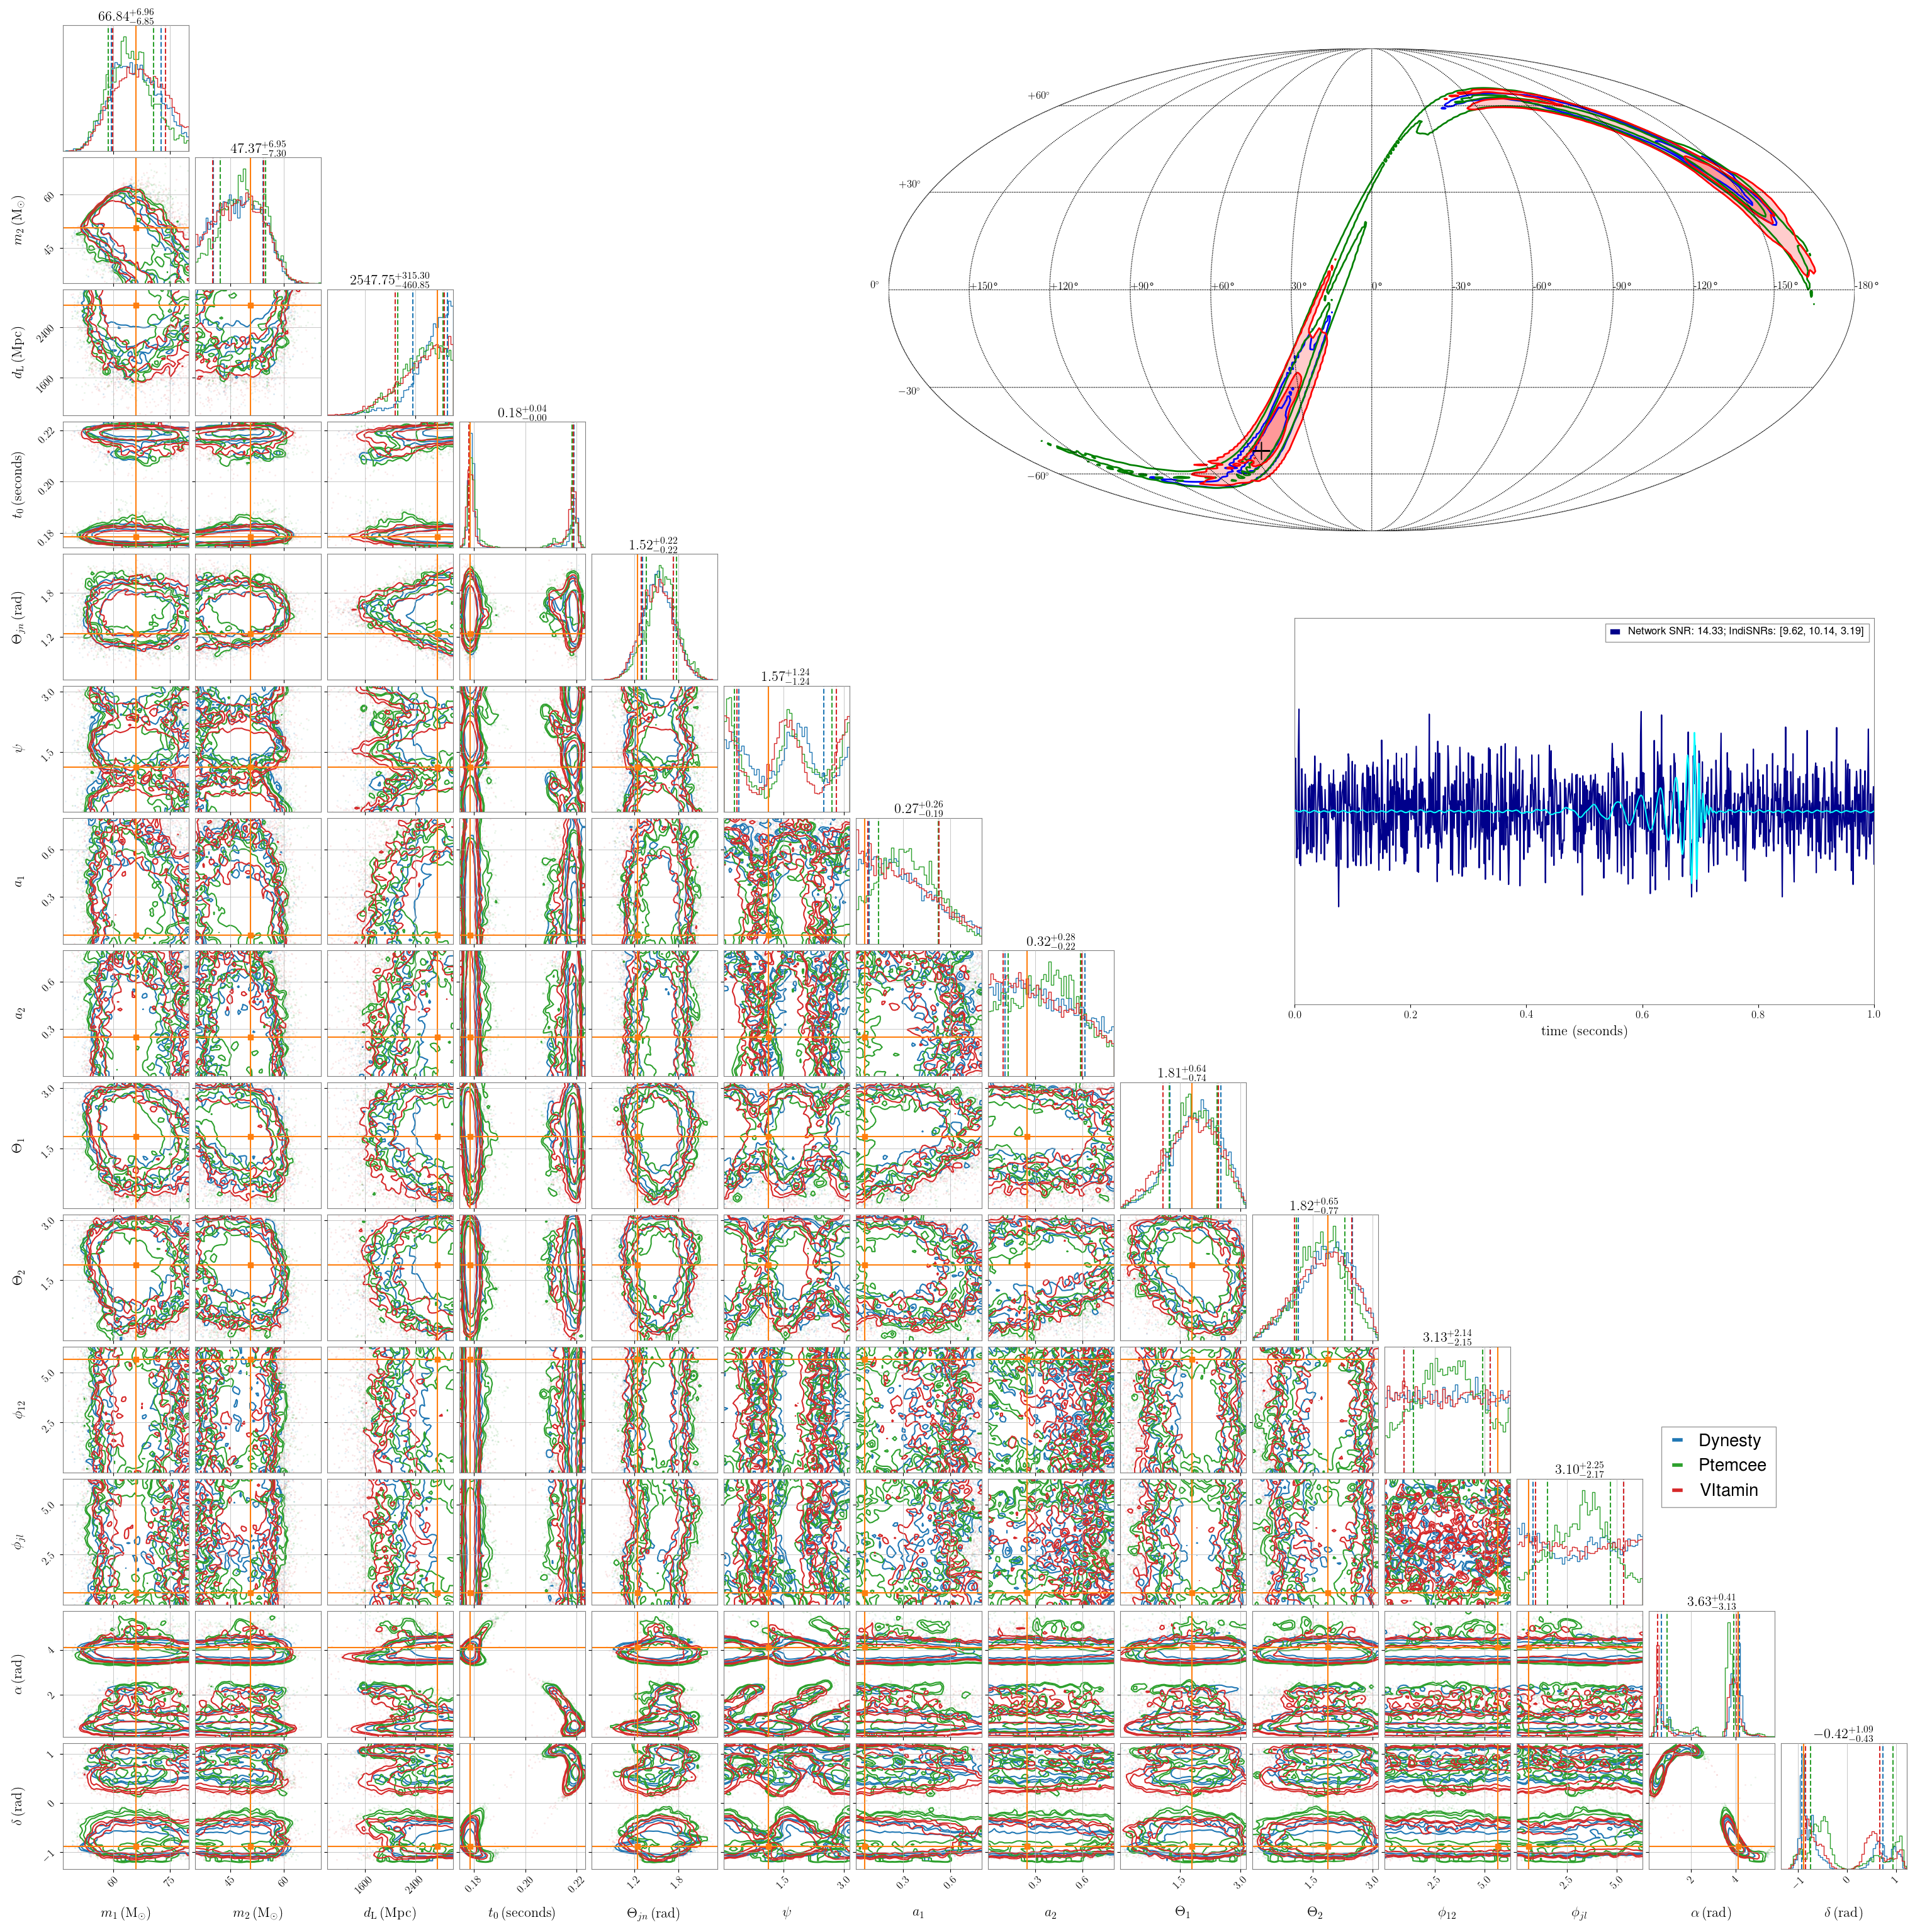
\includegraphics[width=\textwidth]{corner_testcase0.png}
    \caption[Corner plot showing 2 and 1-dimensional
marginalised posterior distributions for one example test dataset from \texttt{VItamin}.]{\label{fig:corner_plot} Corner plot showing 2 and 1-dimensional
marginalised posterior distributions for one example test dataset. Filled (red)
contours represent the posteriors obtained from the \ac{CVAE} approach and
solid (blue) contours are the posteriors output from our baseline analysis
(\texttt{Bilby} using the dynesty sampler). In each case, the contour boundaries
enclose $68,90$ and $95\%$ probability. One dimensional histograms of the
posterior distribution for each parameter from both methods are plotted along
the diagonal. Blue and red vertical lines represent the $5$---$95\%$ symmetric
confidence bounds for \texttt{Bilby} and variational inference respectively.
Black crosses and vertical black lines denote the true parameter values of the
simulated signal. The original whitened noisy timeseries $y$ and the noise-free
signal are plotted in blue and cyan respectively in the upper right hand
panel. The test signal was simulated with optimal signal-to-noise ratio of
13.9.}
\end{figure*}

%
% discuss the corner plot results
%
We can immediately illustrate the accuracy of our machine learning predictions
by directly plotting 2 and 1-dimensional marginalised posteriors generated
using the output samples from our \ac{CVAE} and \texttt{Bilby} approaches
superimposed on each other. We show this for one example test dataset in
Fig.~\ref{fig:corner_plot} where the strong agreement between both
\texttt{Bilby} (blue) and the \ac{CVAE} (red) is clear. 

%We provide additional test case example corner plots in the methods
%section. 
%\hunter{Add more corner plots in methods
%section}~\chris{Maybe, but more corner plots aren't going to convince people.
%We need to agregate the results into a single figure somehow (like the KL
%values). I think something based on the 1-D intervals would be nice.}

%
% mention the pp plot and KL distribution results
%

\textcolor{red}{
A standard test used within the \ac{GW} parameter estimation community is the
production of so-called \ac{PP} plots which we show for our analysis in
Fig.~\ref{fig:pp_plot}. The plot is constructed by computing a p-value for each
output test posterior on a particular parameter evaluated at the true
simulation parameter value (the fraction of posterior samples $>$ the
simulation value). We then plot the cumulative distribution of these
values~\cite{1409.7215}. Curves consistent with the black dashed diagonal line
indicate that the 1-dimensional Bayesian probability distributions are
consistent with the frequentist interpretation - that the truth will lie within
an interval containing $X\%$ of the posterior probability with a frequency of
$X\%$ of the time. It is clear to see that our new approach shows deviations
from the diagonal that are entirely consistent with those observed in all
benchmark samplers. In Fig.~\ref{fig:kl_results} (see Sec.~\ref{sec:methods})
we also show distributions of the \ac{KL} divergence statistic between all
samplers on the joint posterior distributions. It is also clear that the
\ac{KL} divergences between \texttt{VItamin} and any other sampler are
consistent with the distributions between any 2 existing benchmark samplers. 
}

%
% discuss the speed of the analysis
%
The dominating computational cost of running \texttt{VItamin} lies in the \textcolor{red}{
training time, which can take of order several hours to complete.  Completion
is determined by comparing posteriors produced by the machine learning model
and those of \texttt{Bilby} iteratively during training. We additionally assess
whether the cost curves (Fig.~\ref{fig:loss_log}) have converged, such that 
their slope is near-zero. We use a 
single Nvidia Tesla V100 \acp{GPU} with $16/32$ Gb of RAM although consumer grade
``gaming" \ac{GPU} cards are equally fast for this application. 

We stress that
once trained, there is no need to retrain the network unless the user wishes to
use different priors $p(x)$ or assume different noise characteristics.   The
speed at which posterior samples are generated for all samplers used, including
\texttt{VItamin}, is shown in Table~\ref{Tab:speed}. Run-time for the benchmark
samplers is defined as the time to complete their analyses when configured
using their default parameters~\cite{1811.02042}. For \texttt{VItamin} this
time is defined as the total time to produce $3000$ samples. For our test case
of \ac{BBH} signals \texttt{VItamin} produces samples from the posterior at a
rate which is $\sim 6$---$7$ orders of magnitude faster than our benchmark analysis 
using current inference techniques, representing a dramatic speed-up in performance.}

%\chris{One more thing to add, especially if the other KL, AD, and PP plots
%aren't convincing, is a plot displaying 1D confidence bounds compared between
%bilby and VItamin. Imagine a plot with the x-axis as distance and the y-axis
%steps through test data with increasing true distance. for each test data you
%plot 2 error bars horizontally (one for bilby and one for VItamin) spanning the
%range of 90\% confidence. You would hopefully get nearly identical pairs of
%errorbars stacked vertically. Technically you could do this for all parameters
%(and you should) but we might only put one of the plots in the paper (if at
%all).}

%
% I feel the need, the need for speed, table
% 
\begin{table}
\centering
\caption[Durations required to produce samples from each of
the different posterior sampling approaches.]{Durations required to produce samples from each of
the different posterior sampling approaches.}
\begin{tabular}[t]{lcccc}
\toprule
\multirow{2}{*}{sampler} & \multicolumn{3}{c}{run time (seconds)} & \multirow{2}{*}{ratio
$\displaystyle\frac{\tau_{\text{VItamin}}}{\tau_{X}}$} \\
& min & max & median & \\
\hline
Dynesty\footnote{The benchmark samplers all produced $\mathcal{O}(3000-
	10000)$ samples dependent on the default sampling parameters used.} & 602 & 1538 & 774\footnote{The reader may note that benchmark sampler run times are a few orders of magnitude lower than what is typical of a complete \ac{BBH} analysis ($\mathcal{O}(10^{4} -10^{5})$ seconds). This is primarily due our use of a reduced parameter space, low sampling rate and choice of sampler hyperparameters.} & $2.6\times 10^{-6}$ \\
Emcee & 2005 & 11927 & 4351 & $4.6\times 10^{-7}$ \\
Ptemcee & 3354 & 12771 & 4982 & $4.0\times 10^{-7}$ \\
Cpnest & 1431 & 5405 & 2287 & $8.8\times 10^{-7}$ \\
\texttt{VItamin}\footnote{For the \texttt{VItamin} sampler $3000$ samples are
produced as representative of a typical posterior. The run time is independent
of the signal content in the data and is therefore constant for all test cases.} & \multicolumn{3}{c}{\bm{$2\times 10^{-3}$}} & 1 \\
\botrule
\end{tabular}
\label{Tab:speed}
\end{table}

%
% word count ~960 - approx 9.6 words per line
%

%%%%%%%%%%%%%%%%%%%%%%%%%%%%%%%%%%%%%%%%%%%%%%%%%%%%%%%%%%%%%%%%%%%%%%
% CONCLUSIONS
%%%%%%%%%%%%%%%%%%%%%%%%%%%%%%%%%%%%%%%%%%%%%%%%%%%%%%%%%%%%%%%%%%%%%%
%
% conclusions - now draw conclusions about the quality of the comparison
% results. Highlight the current limitations but also highlight the importance of
% this for the GW field (multi-detector is easy, additional parameters are easy,
% longer datasets may be a challenge regarding GPU memory?, we don't have to
% assume a noise model if we inject training data into real noise, we do rely on
% well defined signal models, EM-follow up in very low latency, can we use
% transfer learning if we want to retrain, ...) End with broader statements about
% inference in other fields and how this is applicable across the sciences.
%
% recap and main result
%
\section{Conclusions}
\textcolor{red}{
There are currently a variety of challenges within the field of \ac{GW}
parameter estimation including, and not limited to, accounting for detector
artefacts (non-Gaussian transient "glitches") in the data, time-dependent
variations (non-stationarity) of the detector noise power spectrum density,
systematic uncertainties in the waveform models themselves and decreasing the
latency with which parameter estimates are produced~\cite{1409.7215}. In this
letter we have demonstrated that we are able to reproduce, to a high degree of
accuracy, Bayesian posterior probability distributions generated through
machine learning. This is accomplished using \acp{CVAE} trained on simulated
\ac{GW} signals and does not require the input of precomputed posterior
estimates. We have demonstrated that our neural network model which, when
trained, can reproduce complete and accurate posterior estimates in}
$\mathcal{O}(1)$ millisecond, can achieve the same quality of results as the
trusted benchmark analyses used within the LIGO-Virgo Collaboration.

%
% CBC implications and why this is a game-changer - speed for EM followup
%
\textcolor{red}{
The significance of our results is most evident in the orders of magnitude
increase in speed over existing approaches. This will help the
LIGO-Virgo collaboration alert \ac{EM} follow-up partners with minimum latency, 
enabling tightly coupled, closed-loop control of sensing resources, for maximum information gain.
Improved low-latency alerts will be especially pertinent for signals from
\ac{BNS} mergers (e.g. GW170817~\cite{PhysRevLett.119.161101}) and \ac{NSBH} signals where
parameter estimation speed will no longer be limiting factor\footnote{The complete
low-latency pipeline includes a number of steps. The process of \ac{GW} data
acquisition is followed by the transfer of data. There is then the corresponding
analysis and the subsequent communication of results to the \ac{EM} astronomy
community after which there are physical aspects such as slewing observing
instruments to the correct pointing.} in observing the prompt \ac{EM} emission
expected on shorter time scales than is achievable with existing \ac{LVC}
analysis tools such as Bayestar~\cite{2016PhRvD..93b4013S}.}

%
% CBC implications and why this is a game-changer - faster, modular
%
The predicted number of future detections of \ac{BNS} mergers ($\sim
180$~\cite{2018LRR....21....3A}) will severely strain the \ac{GW} community's
current computational resources using existing Bayesian methods. Future
iterations of our approach will provide full-parameter estimation on \ac{CBC}
signals in $<1$ second on a single \ac{GPU}. Our trained network is also
modular, and can be shared and used easily by any user to produce results. The
specific analysis described in the letter assumes a uniform prior on the signal
parameters. However, this is a choice and the network can be trained with any
prior the user demands, or users can cheaply resample accordingly from the
output of the network trained on the uniform prior. We also note that our
method will be invaluable for population studies since populations may now be
generated and analysed in a full-Bayesian manner on a vastly reduced time
scale. 

%
% future work, current limitations and prospects
%
For \ac{BBH} signals, \ac{GW} data is usually sampled at $1$---$4$ kHz
dependent upon the mass of binary. We have chosen to use the noticeably low
sampling rate of 256Hz and a single detector configuration largely in order to
decrease the computational time required to develop our approach. We do not
anticipate any problems in extending our analysis to higher sampling
frequencies other than an increase in training time and a larger burden on the
\ac{GPU} memory. Our lower sampling rate naturally limited the chosen \ac{BBH}
mass parameter space to high mass signals. We similarly do not anticipate that
extending the parameter space to lower masses will lead to problems but do
expect that a larger number of training samples may be required. Future work
will incorporate a multi-detector configuration at which point parameter
estimation will be extended to sky localisation. 

%
% Non gaussian noise and the final statement
%
\textcolor{red}{
In reality, \ac{GW} detectors are affected by non-Gaussian noise artefacts. To
account for this noise within our scheme, we would train our network using
samples of real detector noise (preferably recent examples to best reflect the
state of the detectors). Our method has the added advantage of not being
dependent on the choice of \ac{PSD} used for whitening, unlike current Bayesian
methods. The whitening procedure applied to the training data for the \ac{CVAE}
is simply to rescale the input to a scale more suitable to neural networks
whereas for existing methods assumptions on the \ac{PSD} directly affect the
posterior results. Our work can naturally be expanded to include the full range
of \ac{CBC} signal types but also to any and all other parameterised \ac{GW}
signals and to analyses of \ac{GW} data beyond that of ground based
experiments. Given the abundant benefits of this method, we hope that a variant
of this of approach will form the basis for all \ac{GW} parameter estimation
over the next several decades to come.}
%
% word count ~620
%

%
% word count 80 
%


%% Here is the endmatter stuff: Supplementary Info, etc.
%% Use \item's to separate, default label is "Acknowledgements"

%%%%%%%%%%%%%%%%%%%%%%%%%%%%%%%%%%%%%%%%%%%%%%%%%%%%%%%%%%%%%%%%%%%%%%
% METHODS
%%%%%%%%%%%%%%%%%%%%%%%%%%%%%%%%%%%%%%%%%%%%%%%%%%%%%%%%%%%%%%%%%%%%%%
%
% methods - Everything that we couldn't fit in. Mostly validation plots.
%
\section{Methods}\label{sec:methods}
%
%Put methods in here.  If you are going to subsection it, use
%\verb|\subsection| commands.  Methods section should be less than
%800 words and if it is less than 200 words, it can be incorporated
%into the main text.

%
% What is an autoencoder?
%
Conditional variational autoencoders are a form of variational autoencoder
which are conditioned on an observation, where in our case the observation is a
1-dimensional \ac{GW} time series signal $y$. The autoencoders from which
variational autoencoders are derived are typically used for problems involving
image reconstruction and/or dimensionality reduction. They perform a regression
task whereby the autoencoder attempts to predict its own given input (model the
identity function) through a ``bottleneck layer'', a limited  and therefore distilled representation of
the input parameter space. An autoencoder is composed of two neural networks,
an encoder and a decoder~\cite{gallinari1987memoires}. %\cite{LIOU20083150}. 
The encoder network takes as
input a vector, where the number of dimensions is a fixed number predefined by
the user. The encoder converts the input vector into a (typically) lower
dimensional space, referred to as the {\it{latent space}}. A representation of
the data in the latent space is passed to the decoder network which generates a
reconstruction of the original input data to the encoder network. Through
training, the two sub-networks learn how to efficiently represent a dataset
within a lower dimensional latent space which will take on the most important
properties of the input training data. In this way, the data can be compressed
with little loss of fidelity. Additionally, the decoder simultaneously learns
to decode the latent space representation and reconstruct that data back to its
original form (the input data).

%
% What is a variational autoencoder?
%
The primary difference between a variational autoencoder~\cite{1812.04405} and
an autoencoder concerns the method by which locations within the latent space
are produced. In our variant of the variational autoencoder, the output of the
encoder is interpreted as a set of parameters governing statistical
distributions (in our case the means and variances of multivariate Gaussians).
In proceeding to the decoder network, samples from the latent space ($z$) are
randomly drawn from these distributions and fed into the decoder, therefore
adding an element of variation into the process. A particular input can then
have a range of possible outputs. In both the decoder and the encoder networks
we use fully-connected layers (although this is not a constraint and any
trainable network architecture may be used).

%%%%%%%%%%%%%%%%%%%%%%%%%%%%%%%%%%%%%%%%%%%%%%%%%%%%%%%%%%%%%%%%%%%%%%
\subsection{Cost function derivation}
%
% A description of the loss function derivation 
%
We will now derive the cost function and the corresponding network structure
and we begin with the statement defining the aim of the analysis. We wish to
obtain a function that reproduces the posterior distribution (the probability
of our physical parameters $x$ given some measured data $y$). The cross entropy
between 2 distributions is defined in Eq.~\ref{eq:cross_ent} where we have made
the distributions explicitly conditional on $y$ (our measurement). In this case
$p(x|y)$ is the target distribution (the true posterior) and $r_{\theta}(x|y)$
is the parametric distribution that we will use neural networks to construct.
The variable $\theta$ represents the trainable neural network parameters. 

The cross-entropy is minimised when $p(x|y)=r_{\theta}(x|y)$ and so by
minimising
%
\begin{align}\label{eq:cost1}
H &= -\text{E}_{p(y)}\left[\int dx\,p(x|y) \log r_{\theta}(x|y)\right],
\end{align}
% 
where $\text{E}_{p(y)}[\cdot]$ indicates the expectation value over the
distribution of measurements $y$, we therefore make the parametric distribution
as similar as possible to the target for all possible measurements $y$.

Converting the expectation value into an integral over $y$ weighted by $p(y)$
and applying Bayes' theorem we obtain
%
\begin{align}\label{eq:cost1}
H &= -\int dx\,p(x)\int dy\,p(y|x)\log r_{\theta}(x|y)
\end{align}
%
where $p(x)$ is the prior distribution on the physical parameters $x$.

The \ac{CVAE} network outlined in Fig.~\ref{fig:network_config} makes use of a
conditional latent variable model and our parametric model is constructed from
the product of 2 separate distributions marginalised over the latent space
%
\begin{align}\label{eq:latent_model}
r_{\theta}(x|y) &= \int dz\,r_{\theta_{1}}(z|y)r_{\theta_{2}}(x|z,y).
\end{align}
%  
We have used $\theta_{1}$ and $\theta_{2}$ to indicate that the 2 separate
networks modelling these distributions will be trained on these parameter sets
respectively. Both new conditional distributions are modelled as $n_{z}$
dimensional multivariate uncorrelated Gaussian distributions (governed by their
means and variances). However, this still allows $r_{\theta}(x|y)$ to take a
general form (although it does limit it to be unimodal).  

One could be forgiven in thinking that by setting up networks that simply aim
to minimise $H$ over the $\theta_{1}$ and $\theta_{2}$ would be enough to solve
this problem. However, as shown in~\cite{NIPS2015_5775} this is an intractable
problem and a network cannot be trained directly to do this. Instead we define
a recognition function $q_{\phi}(z|x,y)$ that will be used to derive an
\ac{ELBO}. Here we use $\phi$ to represent the trainable parameters of an
encoder network ($\text{E}_{2}$).

Let us first define the \ac{KL} divergence between 2 of our
distributions as
%
\begin{align}\label{eq:kl}
\text{KL}&\left[q_{\phi}(z|x,y)||r_{\theta_{2}}(z|x,y)\right] = \\
&\int dz\,q_{\phi}(z|x,y)
\log\left(\frac{q_{\phi}(z|x,y)}{r_{\theta_{2}}(z|x,y)}\right).\nonumber
\end{align}
%  
It can be shown, after some manipulation, that
%
\begin{align}\label{eq:elbo1}
\log r_{\theta}(x|y) &= L + \text{KL}\left[q_{\phi}(z|x,y)||r_{\theta_{?}}(z|x,y)\right],
\end{align}
%
where the \ac{ELBO} $L$ is given by
%
\begin{align}\label{eq:elbo2}
L &= \int dz\,
q_{\phi}(z|x,y)\log\left(\frac{r_{\theta_{2}}(x|z,y)r_{\theta_{1}}(z|y)}{q_{\phi}(z|x,y)}\right)
\end{align}
%
and is so-named since $\text{KL}$ cannot be negative and has a minimum of zero.
Therefore, if we were to find a $q_{\phi}(z|x,y)$ function (optimised on
$\phi$) that minimised the \ac{KL}-divergence then we can state that
%
\begin{align}
\log r_{\theta}(x|y) &\geq L.
\end{align}
%
After some further manipulation of Eq.~\ref{eq:elbo2} we find that
%
\begin{align}\label{eq:logr}
\log r_{\theta}(x|y) \geq  &\text{E}_{q_{\phi}(z|x,y)}\left[\log
r_{\theta_{2}}(x|z,y)\right] \nonumber\\
&-\text{KL}\left[q_{\phi}(z|x,y)||r_{\theta_{1}}(z|y)\right].
\end{align}
%
We can now substitute this inequality into Eq.~\ref{eq:cost1} (our cost
function) to obtain
%
\begin{align}\label{eq:cost2}
H \leq  -\int dx\, p(x)\int dy &\,p(y|x)
\Big[\text{E}_{q_{\phi}(z|x,y)}\left[\log r_{\theta_{2}}(x|z,y)\right]
\nonumber\\
&-\text{KL}\left[q_{\phi}(z|x,y)||r_{\theta_{1}}(z|y)\right]\Big],  
\end{align}
%
which can in practice be approximated as a stochastic integral over draws of
$x$ from the prior, $y$ from the likelihood function $p(y|x)$, and from the
recognition function, giving us Eq.~\ref{eq:cost3}, the actual function
evaluated within the training procedure.

%
% loss plot
%
\begin{figure}
    \includegraphics[width=\columnwidth]{inv_losses_log.png}
\caption[The \texttt{VItamin} cost as a function of training iteration.]{\label{fig:loss_log} The cost as a function of training iteration. We
show the \ac{ELBO} cost function component (blue), the \ac{KL} divergence
component (orange) and total cost (green). The total cost is simply a
summation of the 2 components and one training iteration is defined as
training over one batch of signals.}
\end{figure}

%
% Priors
%
\begin{table}
\centering
\caption[The uniform prior boundaries and fixed parameter values used on the \ac{BBH} signal parameters for the benchmark
and the \ac{CVAE} analyses.]{The uniform prior boundaries and fixed parameter values used on the \ac{BBH} signal parameters for the benchmark
and the \ac{CVAE} analyses.}
\begin{tabular}[t]{lcccc}
\toprule
Parameter name & symbol & min & max & units \\
\hline
mass 1 & $m_1$ & 35 & 80 & solar masses \\
mass 2 & $m_2$\footnote{Additionally $m_2$ is constrained such that
$m_{2}<m_{1}$.} & 35 & 80 & solar masses \\
luminosity distance & $d_{\text{L}}$ & 1 & 3 & Gpc \\
time of coalescence & $t_{0}$ & 0.65 & 0.85 & seconds \\
phase at coalescence & $\phi_{0}$ & 0 & $2\pi$ & radians \\
\hline
right ascension & $\alpha$ & \multicolumn{2}{c}{1.375} & radians \\
declination & $\delta$ & \multicolumn{2}{c}{-1.2108} & radians \\
inclination & $\iota$ & \multicolumn{2}{c}{0} & radians \\
polarisation & $\psi$ & \multicolumn{2}{c}{0} & radians \\
spins & - & \multicolumn{2}{c}{0} & - \\
epoch & - & \multicolumn{2}{c}{1126259642} & GPS time \\
detector & - & \multicolumn{2}{c}{LIGO Hanford} & - \\
\botrule
\end{tabular}
\label{tab:prior_ranges}
\end{table}

%%%%%%%%%%%%%%%%%%%%%%%%%%%%%%%%%%%%%%%%%%%%%%%%%%%%%%%%%%%%%%%%%%%%%%
\subsection{The training procedure}
%
% Introduce the training process
%
Having set up a cost function composed of 3 probability functions that have
well defined inputs and outputs where the mapping of those inputs to outputs is
governed by the parameter sets $\theta_{1},\theta_{2},\phi$. These parameters
are the weights and biases of 3 neural networks acting as (variational)
encoder, decoder, and encoder respectively. To train such a network one must
connect the inputs and outputs appropriately to compute the cost function $H$
and back-propagate cost function derivatives to update the network parameters.
The network structure shown schematically in Fig.~\ref{fig:network_config}
shows how for a batch of $N$ sets of $x$ and corresponding $y$ values, the cost
function is computed during each iteration of training. 

%
% Go through the training step by step
%
Training is performed via a series of steps illustrated in
Fig.~\ref{fig:network_config}.
%
\begin{itemize}
%
\item The encoder $\textrm{E}_1$ is given a set of training \ac{GW} signals
($y$) and encodes $y$ into a set of variables $\mu_q$ defining a distribution
in the latent space. In this case $\mu_q = (\mu_{q0},\sigma^{2}_{q})$ describes
the first 2 central moments (mean and variance) for each dimension of a
uncorrolated (diagonal covariance) multivariate Gaussian distribution.
%
\item The encoder $\textrm{E}_2$ takes a combination of both the data $y$ and
the true parameters $x$ defining the \ac{GW} signal and encodes this into
parameters defining another uncorrelated multivariate Gaussian distribution in
the same latent space. These parameters we denote by
$\mu_{r}=(\mu_{r0},\sigma^{2}_{r})$ again representing the means and variances.
%
\item We then sample from the distribution described by $\mu_{q}$ giving us
samples $z_{q}$ within the latent space.
%
\item These samples, along with their corresponding $y$ data, then go to the
decoder D which outputs $\mu_{x}=(\mu_{x0},\sigma^{2}_{q})$, a set of parameters (much like
$\mu_q,\mu_r$) that define the moments of an uncorrelated  multivariate Gaussian
distribution in the physical $x$ space.
 %
\item The first term of the loss function (Eq.~\ref{eq:cost3}) is then computed
by evaluating the probability density defined by $\mu_x$ at the true $x$
training values. The component of the loss allows the network to learn how to
predict accurate values of $x$ but to also learn the intrinsic variation due to
the noise properties of the data $y$. It is important to highlight that the
\ac{GW} parameter predictions from the decoder D do describe a multivariate
Gaussian, but as is shown in our results (see Fig.~\ref{fig:corner_plot}), this
does \emph{not} imply that our final output posterior estimates will also be
multivariate Gaussians.
%
\item Finally the loss component described by the \ac{KL} divergence between the
distributions described by $\mu^{q}$ and $\mu^{r}$ is computed using
%
\begin{align}\label{eq:klgauss}
\text{KL}&\left[q_{\phi}(z|x_{n},y_{n})||r_{\theta_{1}}(z|y_{n})\right] = \\
&\frac{1}{2}\sum_{j=1}^{n_{z}}\left[\frac{\sigma_{q,j}^{2}}{\sigma_{r,j}^{2}} +
\frac{(\mu_{r0,j}-\mu_{q0,j})^{2}}{\sigma_{r,j}^{2}}+
\log\left(\frac{\sigma_{r,j}^{2}}{\sigma_{q,j}^{2}}\right)\right] -
\frac{n_{z}}{2}.\nonumber 
\end{align}
%
Here we highlight that we do not desire that the network tries to make these 2
distributions equal to each other. Rather, we want the ensemble network to
minimise the total cost (of which this is a component).
%
\end{itemize}

%
% Some practical aspects of the training
%
As is standard practice in machine learning applications, the cost is computed
over a batch of training samples and repeated for a pre-defined number of
iterations. Completion of training is determined by comparing output posteriors
on test samples with those of \texttt{Bilby} iteratively during training. This
comparison is done using standard figures of merit such as the \ac{KL}
divergence and the P-P plot. We also assess training completion based on
whether the cost function and its component parts (Fig.~\ref{fig:loss_log})
have converged. We use a single Nvidia Tesla V100 \acp{GPU} with $16/32$ Gb of
RAM although consumer grade ``gaming" \ac{GPU} cards are equally fast for this
application.


%%%%%%%%%%%%%%%%%%%%%%%%%%%%%%%%%%%%%%%%%%%%%%%%%%%%%%%%%%%%%%%%%%%%%%
\subsection{Network and Training parameters}
%
% Describe the specific network hyper-parameters
%
For our purposes, we found that $\sim3\times10^6$ training iterations, a batch
size of $512$ training samples and a learning rate of $10^{-4}$ was sufficient.
We used a total of $10^6$ training samples in order to adequately cover the
\ac{BBH} parameter space. We additionally ensure that an (effectively) infinite
number of noise realizations are employed by making sure that every time a
training sample is used it is given a unique noise realisation despite only
having a finite number of waveforms. Each neural network ($\text{E}_1$,
$\text{E}_2$, D) is composed of 3 fully connected layers and has $2048$ neurons
in each layer with ReLU~\cite{nair2010rectified} activation functions between
layers. We use a latent space dimension of $8$ and we consider training
complete when both components to the loss function have converged to
approximately constant values or when comparisons with benchmark test
posteriors indicate no significant changes in the output posterior.

%%%%%%%%%%%%%%%%%%%%%%%%%%%%%%%%%%%%%%%%%%%%%%%%%%%%%%%%%%%%%%%%%%%%%%
\subsection{The testing procedure}
%~\chris{Hunter, note that we only need to
%do the first pass through E1 only once for a given piece of data do the real
%cost is only in the other steps. This will likely only change the timing by
%~25\% so it might not be worth doing the tests again. Just bear it in mind.}
%
%
% Introduce the testing procedure
%
After training has completed and we wish to use the network for inference we
follow the procedure described in the right hand panel of
Fig.~\ref{fig:network_config}. Given a new $y$ data sample (not taken from the
training set) we simply input this into the encoder $\textrm{E}_1$ from which we
obtain a single value of $\mu_{r}$ describing a distribution (conditional on the
data $y$) in the latent space. We then repeat the following steps:

%
% Go through the testing step by step
%
\begin{itemize}
%
\item We randomly draw a latent space sample $z_r$ from the latent space
distribution defined by $\mu_r$.
%
\item Our $z_r$ sample and the corresponding original $y$ data are fed as input to our
pre-trained decoder network (D). The decoder network returns a set of moments
$\mu_{x}$ which describe a multivariate Gaussian distribution in the physical
parameter space.
%
\item We then draw a random $x$ realisation from that distribution.
%
\end{itemize}
%

%
% Final testing thoughts
%
A comprehensive representation in the form of samples drawn from the entire joint
posterior distribution can then be obtained by simply repeating this procedure
with the same input data (see Eq.~\ref{eq:latent_model}).

%
% K-L divergence results
%
\subsection{Additional tests}
%
% P-P plot
%
\begin{figure}
    \includegraphics[width=\columnwidth]{latest_pp_plot.png}
    \caption[One-dimensional \ac{PP} plots for each
parameter and each benchmark sampler and \texttt{VItamin}.]{\label{fig:pp_plot} One-dimensional \ac{PP} plots for each
parameter and each benchmark sampler and \texttt{VItamin}.  The curves were
constructed using the 256 test datasets. The dashed black diagonal line
indicates the ideal result.
}
\end{figure}
%

%
% discuss pp plot result
%
%\chris{You need to better describe what a P-P plot is and why we use it. Maybe
%throw in a reference to existing PE group papers that use it. Nature readers
%will have never seen one before. We also have to wait until we get better P-P
%plot curves for our approach before we warrant adding it to the paper.}
A standard test used within the \ac{GW} parameter estimation community is the
production of so-called \ac{PP} plots which we show for our analysis in
Fig.~\ref{fig:pp_plot}. The plot is constructed by computing a $p$-value for each
output test posterior on a particular parameter evaluated at the true
simulation parameter value (the fraction of posterior samples $>$ the
simulation value). We then plot the cumulative distribution of these
values~\cite{1409.7215}. Curves consistent with the black dashed diagonal line
indicate that the 1-dimensional Bayesian probability distributions are
consistent with the frequentist interpretation - that the truth will lie within
an interval containing $X\%$ of the posterior probability with a frequency of
$X\%$ of the time. It is clear to see that our new approach shows deviations
from the diagonal that are entirely consistent with those observed in all
benchmark samplers. 

%
\begin{figure}
    \includegraphics[width=\columnwidth]{hist-kl.png}
    \caption[Distributions of \ac{KL}-divergence values
between posteriors produced by different samplers.]{\label{fig:kl_results} Distributions of \ac{KL}-divergence values
between posteriors produced by different samplers. The \ac{KL} divergence is
computed between all samplers with every other sampler over all 256 \ac{GW}
test cases. The distributions of the resulting \ac{KL} divergence values are
then plotted, with each color representing a different sampler combination
including \texttt{VItamin} as one of the sampler pairs. The grey distributions
represent the results from all benchmark sampler pairs for comparison. Both the
$x$ and $y$ axes are scaled logarithmically for readability.}
\end{figure}
%

%
% discuss the KL results
%
The \ac{KL} divergence between 2 distributions is a measure of their similarity
and we use this to compare the output posterior estimates between samplers for
the same input test data. To do this we run each independent sampler (including
the \ac{CVAE}) on the same test data to produce samples from the corresponding
posterior. We then compute the \ac{KL}-divergence between output distributions
from each sampler with itself and each sampler with all other samplers. For
distributions that are identical the \ac{KL}-divergence is equal to zero but
since we are representing our posterior distributions using finite numbers of
samples, identical distributions should result in KL-divergence values $<1$. In
Fig.~\ref{fig:kl_results} we show the distributions of these
\ac{KL}-divergences for the 256 test \ac{GW} samples where we see that the
\ac{CVAE} approach when compared to the benchmark samplers have distributions
consistent with those produced when comparing between 2 different benchmark
samplers.

\section{Additional analysis}

In the following section we will discuss additional analysis of the results 
from \texttt{VItamin} including: analysis of the JS divergence using individual 
source parameter values, training set \ac{SNR} distribution and it's 
effect on the performance of \texttt{VItamin}, the structure and behavior 
of the \ac{CVAE} latent space and it's effect on the predicted 
posterior distributions, ...

\subsection{JS divergence for individual source parameters}
%
% Individual source parameter JS divergences
%

We provide additional figures of merit in Fig. \ref{fig:JS_indi_par_cpnest}, 
\ref{fig:JS_indi_par_dynesty}, \ref{fig:JS_indi_par_emcee}, \ref{fig:JS_indi_par_ptemcee} where 
we plot the JS divergence values for each \ac{GW} source parameter across all Bayesian 
sampler approaches. Each sampler method vs. another sampler method are 
denoted as different colors. The lower and upper end of boxes represent the 
25th and 75th credibility regions respectively. The lower and upper end of 
the whiskers represent the 5th and 95th percent credibility regions. The 
dashed red line represents optimal JS divergence value according to 
sampler experts ($\sim 0.002$).

%
% Discuss Dynesty plot
%

In Fig. \ref{fig:JS_indi_par_dynesty}, it can be seen that \texttt{Dynesty}  vs. \texttt{VItamin} JS values closely 
matches results from \texttt{Dynesty} vs. \texttt{Ptemcee} for nearly all parameters, with the exception of 
$t_0$, $\theta_{jn}$, $\phi_{jl}$, $\alpha$ and $\delta$. \texttt{VItamin} predictions 
have a slightly higher mismatch across all source parameters except for the spin
parameters. \texttt{Dynesty} vs. CPNest seems to generally have similar JS 
values to \texttt{Dynesty} vs. \texttt{Ptemcee} with the exception of having 
broader credibility intervals on $t_0$, $\theta_{jn}$, $\phi_{jl}$, $\alpha$ 
and $\delta$. \texttt{Dynesty} vs. \texttt{Emcee} generally has higher JS values 
than all other methods, which is expected given the difficulty of 
\texttt{Emcee} convergence.


\begin{figure}
    \includegraphics[width=\columnwidth]{figures/JS_IndiPar_dynesty_nature_paper.png}
    \caption[JS divergences of individual source parameters for \texttt{Dynesty} against all other approaches.]{\label{fig:JS_indi_par_dynesty} Shown are JS divergence values for all test samples as a function of test sample source parameter for \texttt{Dynesty} against every other sampling approach. Each JS value is a 1-dimensional JS statistic, rather than the full 14-dimensional JS statistics shown earlier. Each sampler method vs. another sampler method are denoted as different colors. The lower and upper end of boxes represent the 25th and 75th credibility regions respectively. The lower and upper end of the whiskers represent the 5th and 95th percent credibility regions. The dashed red line represents optimal JS divergence value according to sampler experts ($\sim 0.002$). The orange line is representative of the median JS value. We see here that \texttt{VItamin} performs to within the same degree of accuracy as other Bayesian samplers when looking at predictions on an individual source parameter basis.}
\end{figure}

%
% Discuss CPNest plot
%

In Fig. \ref{fig:JS_indi_par_cpnest}, \texttt{CPNest} is highlighted against 
all other sampler approaches (including \texttt{VItamin}). It can be seen 
that both \texttt{CPnest} vs. \texttt{Dynesty} and \texttt{CPnest} vs. 
\texttt{Ptemcee} are in strong agreement with each other (although with broad 
credibility regions on $t_0$, $\theta_{jn}$, $\alpha$, $\delta$). \texttt{CPNest} 
vs. \texttt{VItamin} is also in strong agreement with \texttt{CPnest} vs. \texttt{Dynesty} and \texttt{CPnest} vs. \texttt{Ptemcee}, but it does show some 
disagreement on $m_1$, $m_2$ and $\psi$. \texttt{CPNest} vs. \texttt{Emcee} is 
generally in disagreement with all other approaches.

\begin{figure}
    \includegraphics[width=\columnwidth]{figures/JS_IndiPar_cpnest_nature_paper.png}
    \caption[JS divergences of individual source parameters for \texttt{CPNest} against all other approaches.]{\label{fig:JS_indi_par_cpnest} Shown are JS divergence values for all test samples as a function of test sample source parameter for \texttt{CPNest} against every other sampling approach. Each JS value is a 1-dimensional JS statistic, rather than the full 14-dimensional JS statistics shown earlier. Each sampler method vs. another sampler method are denoted as different colors. The lower and upper end of boxes represent the 25th and 75th credibility regions respectively. The lower and upper end of the whiskers represent the 5th and 95th percent credibility regions. The dashed red line represents optimal JS divergence value according to sampler experts ($\sim 0.002$). The orange line is representative of the median JS value. We see here that \texttt{VItamin} performs to within the same degree of accuracy as other Bayesian samplers when looking at predictions on an individual source parameter basis.}
\end{figure}

%
% Discuss Emcee JS indi par plot
%

Fig. \ref{fig:JS_indi_par_emcee} highlights the \texttt{Emcee} sampler 
vs. all other approaches including \texttt{VItamin}. In Fig. 
\ref{fig:JS_indi_par_emcee} it can be seen that \texttt{Emcee} has equal 
overlap against all other sampler approaches. Given the high JS values 
of \texttt{Emcee} vs. all other approaches, this indicates that \texttt{Emcee} 
has found difficulty converging on many of the test sample cases. This is 
expected given that it is well known that \texttt{Emcee} generally difficult 
to tune for proper convergence.

\begin{figure}
    \includegraphics[width=\columnwidth]{figures/JS_IndiPar_emcee_nature_paper.png}
    \caption[JS divergences of individual source parameters for \texttt{Emcee} against all other approaches.]{\label{fig:JS_indi_par_emcee} Shown are JS divergence values for all test samples as a function of test sample source parameter for \texttt{Emcee} against every other sampling approach. Each JS value is a 1-dimensional JS statistic, rather than the full 14-dimensional JS statistics shown earlier. Each sampler method vs. another sampler method are denoted as different colors. The lower and upper end of boxes represent the 25th and 75th credibility regions respectively. The lower and upper end of the whiskers represent the 5th and 95th percent credibility regions. The dashed red line represents optimal JS divergence value according to sampler experts ($\sim 0.002$). The orange line is representative of the median JS value. We see here that \texttt{VItamin} performs to within the same degree of accuracy as other Bayesian samplers when looking at predictions on an individual source parameter basis.}
\end{figure}

%
% Discuss Ptemcee JS indi par plot
%

Fig. \ref{fig:JS_indi_par_ptemcee} highlights \texttt{Ptemcee} vs. all 
other sampler approaches. In Fig. \ref{fig:JS_indi_par_ptemcee} we see 
that \texttt{Ptemcee} vs. \texttt{Dynesty} and \texttt{Ptemcee} vs. 
\texttt{CPNest} closely match each other with the exception of slight 
disagreement on $t_0$, $\theta_{jn}$ and $\phi_{jl}$ (with broader credibility regions on \texttt{Ptemcee} 
vs. \texttt{CPNest}). \texttt{Ptemcee} vs. \texttt{VItamin} in dark green 
also closely matches the \texttt{Ptemcee} vs. \texttt{Dynesty} and \texttt{Ptemcee} vs. \texttt{CPNest} results with slightl higher JS values 
accross all source parameter values other than the spin parameters. 
\texttt{Emcee} is in strong misalignment with all other approaches.

\begin{figure}
    \includegraphics[width=\columnwidth]{figures/JS_IndiPar_ptemcee_nature_paper.png}
    \caption[JS divergences of individual source parameters for \texttt{Ptemcee} against all other approaches.]{\label{fig:JS_indi_par_ptemcee} Shown are JS divergence values for all test samples as a function of test sample source parameter for \texttt{Ptemcee} against every other sampling approach. Each JS value is a 1-dimensional JS statistic, rather than the full 14-dimensional JS statistics shown earlier. Each sampler method vs. another sampler method are denoted as different colors. The lower and upper end of boxes represent the 25th and 75th credibility regions respectively. The lower and upper end of the whiskers represent the 5th and 95th percent credibility regions. The dashed red line represents optimal JS divergence value according to sampler experts ($\sim 0.002$). The orange line is representative of the median JS value. We see here that \texttt{VItamin} performs to within the same degree of accuracy as other Bayesian samplers when looking at predictions on an individual source parameter basis.}
\end{figure}

It is evident in Fig's \ref{fig:JS_indi_par_cpnest}, 
\ref{fig:JS_indi_par_dynesty}, \ref{fig:JS_indi_par_emcee}, \ref{fig:JS_indi_par_ptemcee} that JS values for individual source 
parameters of \texttt{VItamin} against all other sampler is generally 
consistent with all other samplers against themselves. This is an important 
point because it indicates that our machine learning approach is able 
to produce Bayesian posteriors to within an accuracy which is at a similar 
level of other Bayesian samplers, using the same individual source 
parameter figure of merit used for other comparison studies in the Bayesian 
\ac{GW} parameter estimation literature \cite{1811.02042,2008.03312,PhysRevD.102.104057}. What is also 
interesting to note is the level of disagreement of other Bayesian samplers 
with themselves. This disagreement is especially prominent with regards 
to source parameters $t_0$, $\theta_{jn}$, $\phi_{jl}$, $\alpha$, and $\delta$.
Although \texttt{Emcee} results are fairly poor in comparison with other 
approaches, they are a useful benchmark for indicating underperformance. 


%
% JS as a function of SNR
%

\subsection{JS divergence as a function of SNR}

Over the course of this project there was some discussion on the possibility 
that \ac{SNR} might be a limiting factor with regards to the performance 
of the neural network model. It was originally hypothesized that due to the 
low number of high \ac{SNR} signals in our training set (as seen in 
Fig. \ref{fig:VItamin_TrainingSet_SNR_Dist}), that the network would perform worse on high \ac{SNR} signals. 
This hypothesis is supported by the well known understanding in 
machine learning literature that less available 
data in specific regions of the parameter space can cause a neural network
model to underfit to those regions \cite{everitt2010cambridge}. As a test, 
we have plotted in Fig. \ref{fig:JS_vs_SNR_dynesty} the JS divergence for 
individual test sample cases of \texttt{VItamin} vs. \texttt{Dynesty} 
as a function of \ac{SNR}. Each plus sign is representative of indivudal test 
cases and different colors correspond to each interferometer. 

\begin{figure}
    \includegraphics[width=\columnwidth]{figures/TrainingSetSNR_distribution.png}
    \caption[VItamin SNR training set distribution.]{\label{fig:VItamin_TrainingSet_SNR_Dist} Shown is a histogram of the \ac{SNR} values of the \texttt{VItamin} training set. There is a peak of signals centered around an \ac{SNR} value of 8 which drops off quickly to zero on the left-hand side. There is a tail on the right-hand side which drops off more gradually up to a maximum \ac{SNR} value of $\sim 70$. The peak location and general distribution of the \ac{SNR} values is heavily dependent on both the chosen source parameter priors and the \ac{PSD}.}
\end{figure}

\begin{figure}
    \includegraphics[width=\columnwidth]{figures/JS_vs_SNR_nature_paper.png}
    \caption[JS divergences of \texttt{Dynesty} vs. \texttt{VItamin} as a function of \ac{SNR}.]{\label{fig:JS_vs_SNR_dynesty} Shown are JS divergence values of \texttt{Dynesty} vs. \texttt{VItamin} as a function of \ac{SNR}. Different colors are representative of each of the 3 detectors (H1, L1, V1) used in the analysis. Each ``plus'' symbol represents a different test \ac{GW} case. As can be seen, there does not appear to be a strong positive correlation with \ac{SNR}. One could argue there is in fact a small negative correlation with network performance and \ac{SNR} value, but this is not clear. }
\end{figure}

We see in Fig. \ref{fig:JS_vs_SNR_dynesty} that there is little to no 
positive correlation between \ac{SNR} and JS divergence. In fact, there 
may be a slight negative correlation. This shows that there would be 
marginal benefit gained from augmenting the training set to more strongly 
emphasize high \ac{SNR} signals. Even if there were a positive correlation 
it is unlikely that simply including more high \ac{SNR} signals would be 
beneficially to the statistical results of the network model as a 
whole because there are fewer test signals at high \ac{SNR} anyways due 
to the priors used.

\subsection{VItamin latent space analysis}

%
% Subsection intro
%
In this section I will introduce diagnostic plots we have used 
in order to gauge the performance of our neural network model with 
respect to the latent space. I will also provide the posterior predictions 
for context for each test sample discussed.

%
% Discuss the corner plot for test case 184.
%
For context, we will first examine a test case at a median network \ac{SNR} 
value of $\sim 14.33$. As seen in Fig. \ref{fig:comp_post_184}, this 
median \ac{SNR} event exhibits complex multi-modal behavior in across 
several dimensions including: $t_0$, $\psi$, $\alpha$ and $\delta$. 
There also appears to some disagreement between Bayesian samplers, 
particularly on the $\phi_{jl}$, $\phi_{12}$ and $a_1$ parameters. 
The sky plot in the upper right-hand corner of Fig. \ref{fig:comp_post_184} 
is also multi-modal and spans a large region of the sky. We will discuss 
in the following paragraphs how latent space predictions translate to 
posterior predctions.

%
% Discuss the latent space corner plots
%

There is no hard rule for determining the number of latent space 
dimensions to use when deciding on the architecture for a \ac{CVAE}. 
That being said, our primary motivation for choosing a latent space size 
of 15 is directly related to the total number of source parameter posteriors 
we are trying to get the neural network model to learn. Our hope was that 
each dimension of the latent space would encode information corresponding 
to each dimension of the posterior space. However, as can be seen 
in Fig. \ref{fig:latent_corner_184}, there are some indications that 
this may not be the case of what's actually happening underneath the 
hood. 

In Fig. \ref{fig:latent_corner_184} we plot $8000$ latent space samples 
drawn from predictions made by both the $q$ (blue) and $r_1$ (red) encoder networks. If a dimension of the latent space is being used, we would expect 
that the corresponding 1-D histogram for that latent space dimension 
along the diagonal of the corner plot to show some level of disagreement 
between the predictions from both encoder networks. The reasoning behind 
this statement is that the $q$ network is given a different level 
of information with respect to the $r_1$ network. Specifically, the 
$q$ network is given not only the \ac{GW} time series, but also 
the true values of the source parameters themselves, whereas the 
$r_1$ network is given the \ac{GW} time series by itself. If a latent space 
dimension is not being used it means that there is no additional 
amount of information that can be gleamed from that dimension, so 
both encoder networks will simply return mean zero unit variate Gaussian 
distributions, which contribute nothing to the loss function. Nothing is 
contributed to the loss function during training because the KL 
divergence between two Gaussian distributions is zero. Since the KL 
component of the loss is zero for this dimension, weights will not 
be updated during the backpropogation process which encourage this 
dimension to be used. 

From Fig. \ref{fig:latent_corner_184} we see that 6 of the 15 latent 
space dimensions are not being used for this test case. It also appears 
that the $r_1$ encoder network (which is capable of producing multi-modal 
distributions) is in fact choosing to, on the whole, produce latent space 
samples which are representative of uni-modal distributions. What this 
implies is that the multi-modality clearly seen in the final posteriors 
of Fig. \ref{fig:comp_post_184} is entirely handled by the $r_2$ decoder 
network which is apprently choosing what level of likelihood to 
assign to each mode in the posterior space. 

This could indicate that the decoder network could have a 
higher level of capacity than what may be needed and is just bypassing 
the Gaussian Mixture Model in the $r_1$ encoder network.

%
% Test set sample 184 corner plot
%
\begin{figure}
    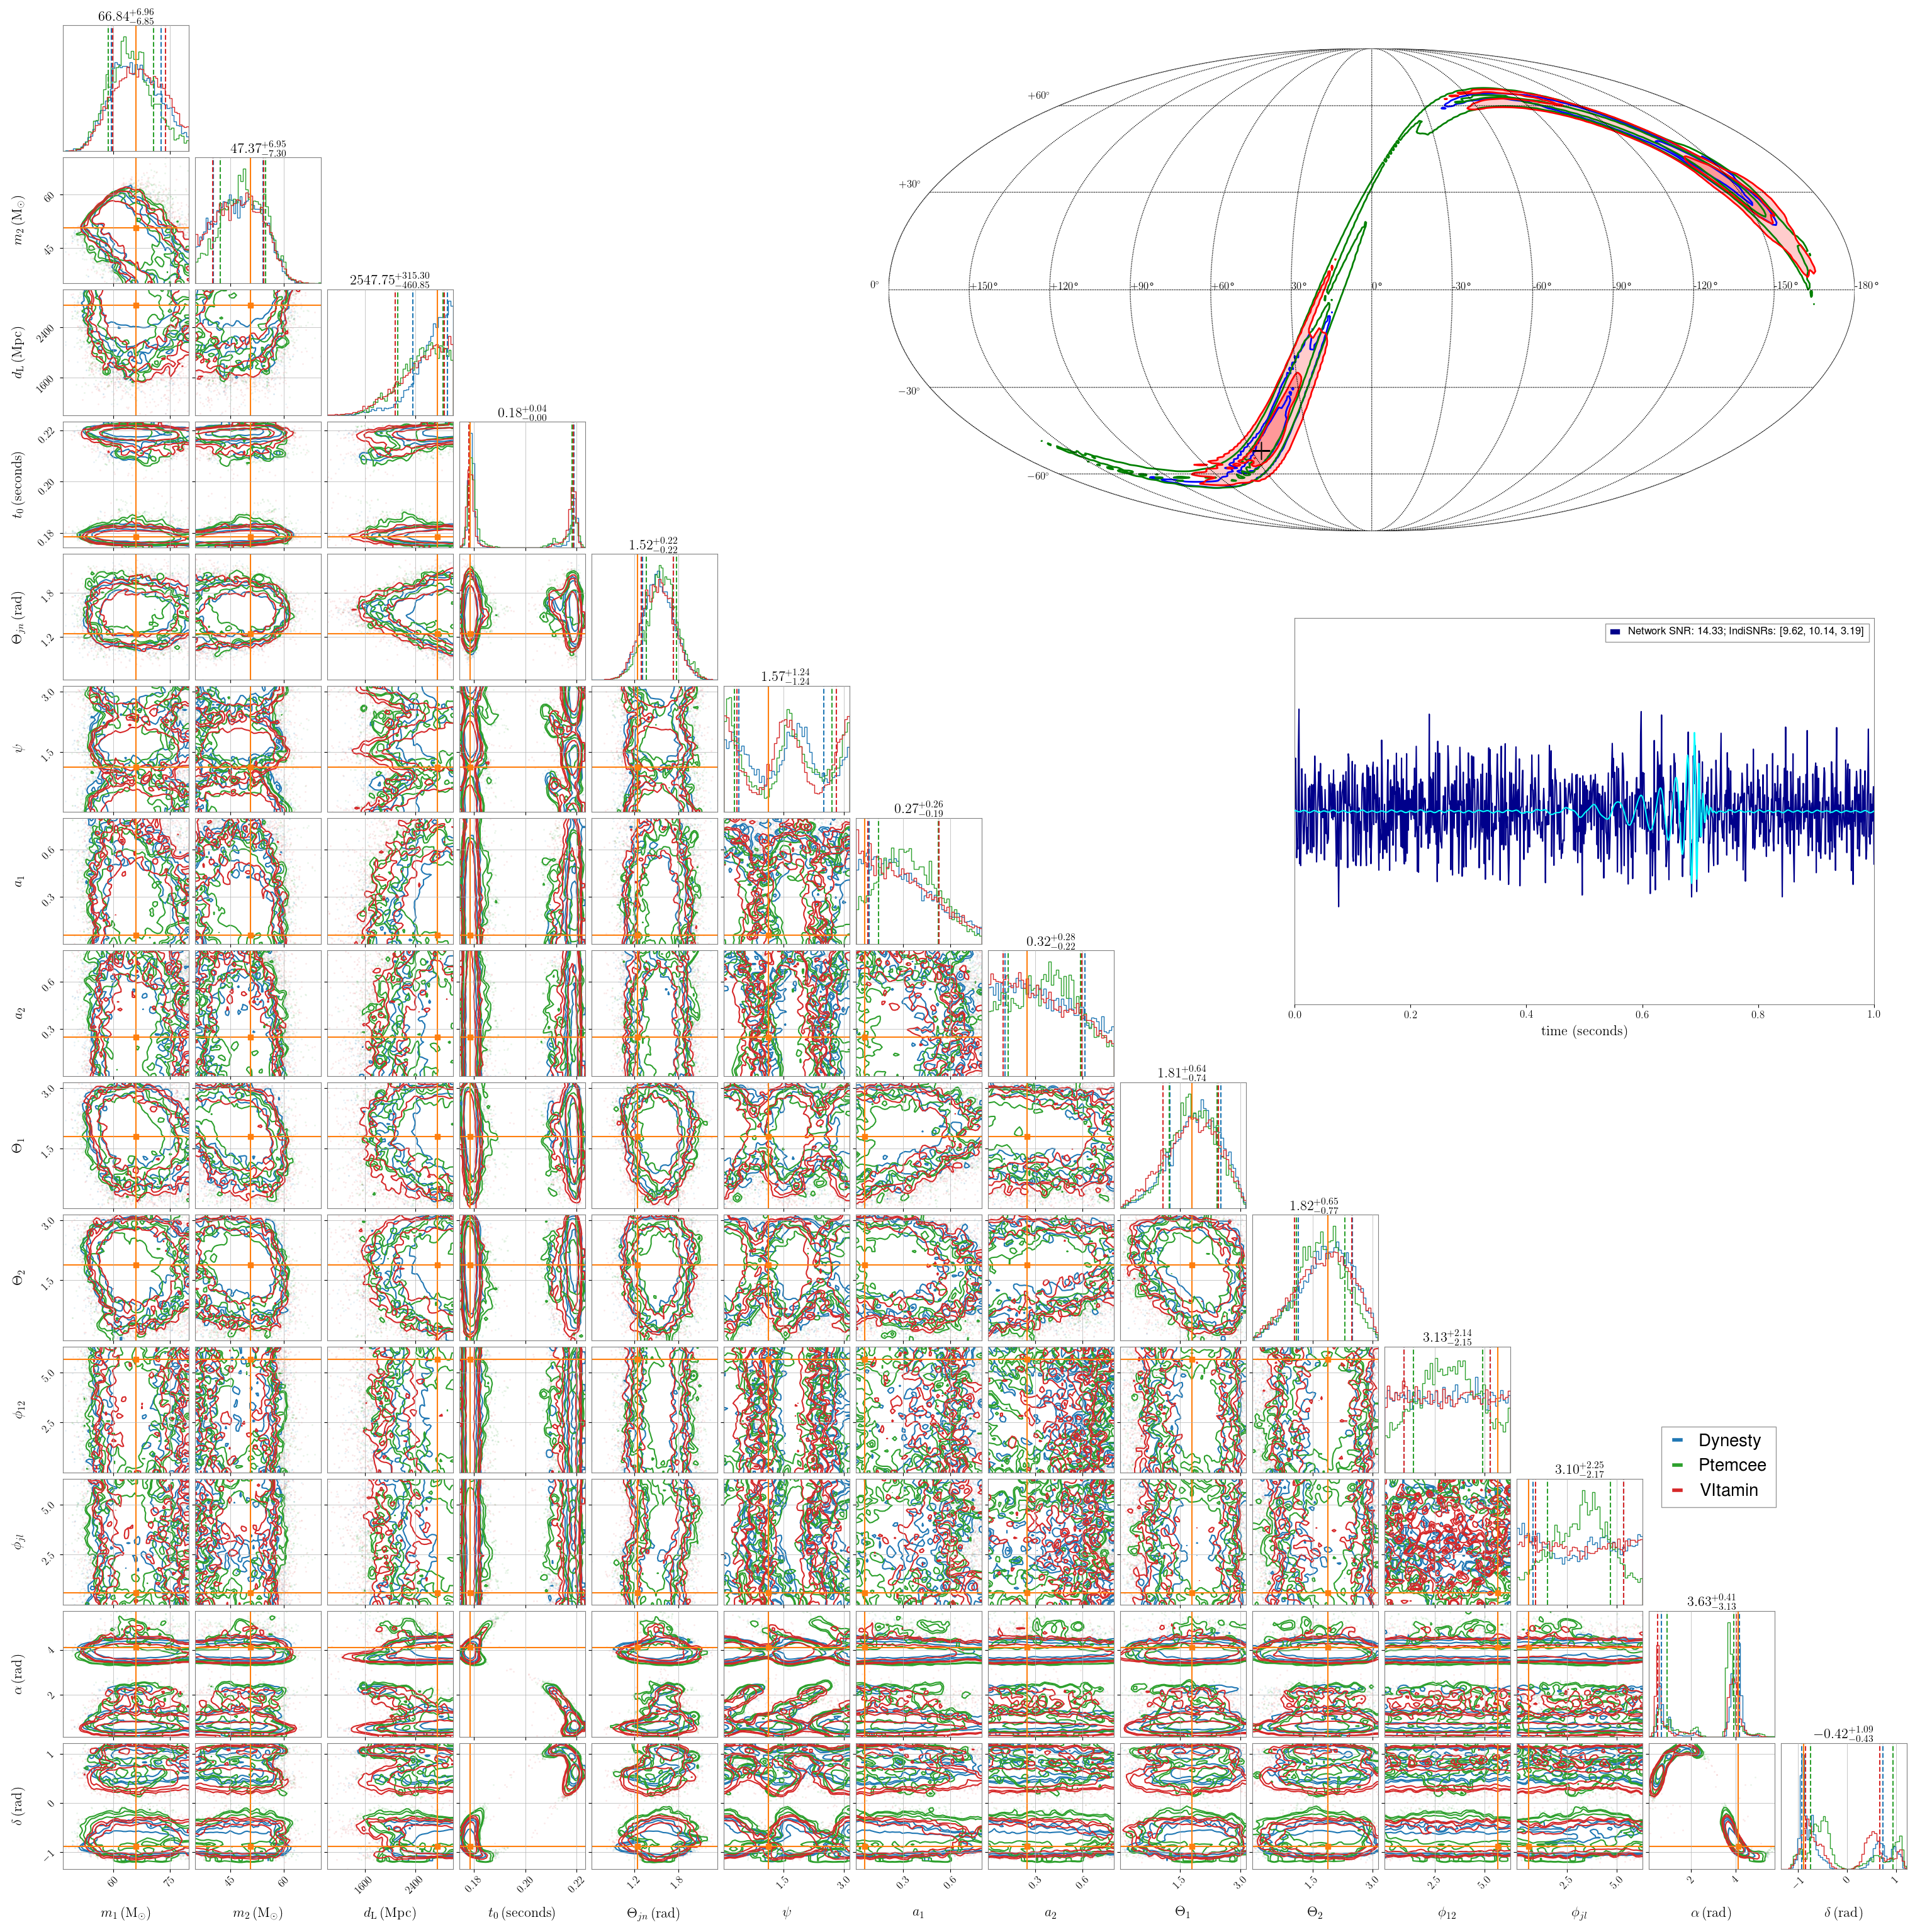
\includegraphics[width=\columnwidth]{figures/comp_posterior_pub_plot_event_184.png}
    \caption[Posterior predictions from \texttt{VItamin}, \texttt{Dynesty} and \texttt{Ptemcee} for the 184th test sample in the \texttt{VItamin} paper training set.]{\label{fig:comp_post_184} Corner plot showing 2 and 1-dimensional marginalised posterior distributions for 184th test dataset sample. Filled (red) contours represent the posteriors obtained from the \ac{CVAE} approach and solid (blue) contours are the posteriors output from our baseline analysis (\texttt{Bilby} using the \texttt{Dynesty} sampler). In each case, the contour boundaries enclose $68,90$ and $95\%$ probability. One dimensional histograms of the posterior distribution for each parameter from both methods are plotted along the diagonal. Blue and red vertical lines represent the $5$---$95\%$ symmetric confidence bounds for \texttt{Bilby} and variational inference respectively. Black crosses and vertical black lines denote the true parameter values of the simulated signal. The original whitened noisy timeseries $y$ and the noise-free signal are plotted in blue and cyan respectively in the upper right hand panel. The test signal was simulated with network optimal signal-to-noise ratio of 14.33.}
\end{figure}

%
% Test sample 184 log weights histogram
%
\begin{figure}
    \includegraphics[width=\columnwidth]{figures/latent_logweight_pub_plot_event_184.png}
    \caption[Latent space log weight plot for the 184th test sample in the \texttt{VItamin} paper training set.]{\label{fig:log_weight_184} Plotted are the predicted log'd weight values for the zeroth posterior sample of the 184th test sample as a function of mode latent space dimension number. Mode weights are predicted for each posterior sample by the $r_1$ encoder network.}
\end{figure}

%
% Test sample 184 latent space samples corner plot
%
\begin{figure}
    \includegraphics[width=\columnwidth]{figures/latent_pub_plot_event_184.png}
    \caption[Latent space samples corner plot for the 184th test sample in the \texttt{VItamin} paper training set.]{\label{fig:latent_corner_184} Shown are $8000$ latent space samples from all latent space dimensions of both 
    the $q$ encoder network (blue) and the $r_1$ encoder network (red). Each square point is representative of the predicted mean values for each latent space dimension (15). Each dimension on the x and y axis represents a different latent space dimension. 1-d histograms of latent space samples for each dimension are plotted along the diagonal. Contours represent the $68, 90, 95\%$ credibility intervals. Blue and red vertical lines denote the $5 - 95\%$ symmetric confidence bounds for the $q$ and $r_1$ networks respectively.}
\end{figure}

%
% Test sample 184 weights histogram
%
\begin{figure}
    \includegraphics[width=\columnwidth]{figures/latent_weight_pub_plot_event_184.png}
    \caption[Latent space weight plot for the 184th test sample in the \texttt{VItamin} paper training set.]{\label{fig:log_weight_184} Plotted are the unlogged predicted weight values from the $r_1$ encoder network for the zeroth posterior sample of the 184th test case as a function of latent space mode dimension number. Each value is normalised to be betweeen 0 and 1 where 1 is representative of the network model assigning a high likelihood of sampling from that particular mode.}
\end{figure}


\subsection{Dynesty vs. Dynesty JS Divergence}

Here we provide some discussion on what the absolute best JS values we 
could hope for from \texttt{VItamin} by comparing two independent Dynesty 
runs on all $250$ test sample cases for both the full 14-dimensional JS 
divergence and the 1-dimensional JS divergence.
%
% Dynesty vs. Dynesty Full JS
%

\begin{figure}
    \includegraphics[width=\columnwidth]{figures/dynesty-dynesty_fullJS.png}
    \caption[Dynesty vs. Dynesty full 14-D JS divergence histogram plot.]{\label{fig:dyn_vs_dyn_ful14D_JS} A histogram of JS divergence values for \texttt{Dynesty} vs. another independent run of \texttt{Dynesty}. The mean JS divergence has a value of $0.05$. We do note that since since the JS statistic is calculated using the \texttt{universal-divergence} code-base, that there are some negative values which are not shown here.}
\end{figure}

%
% Dynesty vs. Dynesty 1D JS
%

\begin{figure}
    \includegraphics[width=\columnwidth]{figures/dynesty-dynesty_indiJS.png}
    \caption[Dynesty vs. Dynesty full 1-D JS divergence histogram plot.]{\label{fig:dyn_vs_dyn_ful14D_JS} Shown are histograms of 1-dimensional JS divergence values for \texttt{Dynesty} vs. another independent run of \texttt{Dynesty}. Different colors represent JS values with respect to individual source parameter posterior \texttt{Dynesty} predictions. Mean JS values for each source parameter are given as: $m_1 \sim 0.00139$, $m_2 \sim 0.00143$, $d_l \sim 0.00142$, $t_0 \sim 0.00358$, $\theta_{jn} \sim 0.00192$, $\psi \sim 0.00134$, $a_1 \sim 0.00101$, $a_2 \sim 0.00088$, $\Theta_1 \sim 0.00143$, $\Theta_2 \sim 0.00123$, $\phi_{12} \sim 0.00080$, $\phi_{jl} \sim 0.00136$, $\alpha \sim 0.00538$, $\delta \sim 0.00401$. JS values are calculated using the \texttt{scipy} JS divergence code-base. }
\end{figure}

\chapter{Conditional variational autoencoders for detecting real GW signals}

In this chapter I will discuss some recent soon to be published work on using the \texttt{VItamin} machine learning for gravitational wave parameter estimation pipeline to do Bayesian PE on real \ac{GW} signals. In the first section I will introduce the problem, in the second I will discuss data pre-processing and generation, in the third section I will discuss results in both real and Gaussian noise cases on a variety of real \ac{GW} signals.

\section{Introduction}

\section{Signal pre-processing/generation}

\section{Training tricks}

\subsection{Data augmentation}

In addition to allowing the network to see multiple noise realizations 
of the same signal multiple times, every time we give the network 
a new chunk of signals, we also randomize the phase, time of arrival and 
distance of the new loaded in training samples.

%
% Distance augmentation
%
For distance, we first choose values uniformly at random from 0 to 1 for 
each distance training sample parameter. These values are then 
converted to units of Mpc by 

\begin{equation}\label{eq:dist_rescale}
    d_{\textrm{new}} = d_{\textrm{min}} + d_{\textrm{uni}}*(d_{\textrm{max}} - d_{\textrm{min}}),
\end{equation}

where $d_{\textrm{uni}}$ is a uniform set of numbers between 0 and 1, 
$d_{\textrm{max}}$ represents the maximum allowed distance according to the prior and $d_{\textrm{min}}$ is the minimum allowed distance according to the prior. We then determine the factor by which the distance has changed from its old value for each training sample by dividing the old distance by the new distance value.

\begin{equation}
    d_{\textrm{corr}} = \frac{d_{\textrm{old}}}{d_{\textrm{new}}}
\end{equation}

where $d_{\textrm{old}}$ is the original distance value for the sample 
and $d_{\textrm{new}}$ is the new value. 

%
% Phase augmentation
%

In order to get the phase augmentation scale term 
we do a similar process as the distance 
augmentation above. We again choose a uniform value between 0 and 1 and 
apply the same rescaling as that in equation \ref{eq:dist_rescale}, but 
instead with bounds relavent to phase (0 to $\pi$). Bounds are only 
up to a maximum of $\pi$ due an applied reparameterization trick 
discussed below in subsection \ref{subsec:phipsi_repar}. A phase 
correction term is then calculated

\begin{equation}
    \phi_{\textrm{corr}} = -1.0 \times (\cos(\phi_{\textrm{new}} - \phi_{\textrm{old}}) + \sin(\phi_{\textrm{new}} - \phi_{\textrm{old}}) \times i),
\end{equation}

where $\phi_{\textrm{corr}}$ is the phase correction factor we 
will use to randomize the phase, $\phi_{\textrm{new}}$ is the new 
randomized phase value and $\phi_{\textrm{old}}$ is the original 
training sample phase value.

%
% time correction
%

The time scale term is then computed by again choosing a random value 
between 0 and 1 for all training samples and rescaling those random 
values to be in units of seconds which are between the allowable 
prior bounds of time. We then convert the new randomized time 
to radians and find the difference between the new and old 
times

\begin{equation}
    t_{\textrm{corr}} = -2.0\pi (t_{\textrm{new}} - t_{\textrm{old}}),
\end{equation}

where $t_{\textrm{new}}$ is the new time of coalescence, $t_{\textrm{old}}$ 
is the old time of coalescence and $t_{\textrm{corr}}$ is the time of coalesence scale factor. The complex value for the time of coalesence 
scale factor $t_{\textrm{corr}}$ is computed 

\begin{equation}
    t_{\textrm{corr}} = -1.0 \times (\cos(t_{\textrm{corr}}) + \sin(t_{\textrm{corr}}) \times i).
\end{equation}

Finally, given all the correction factors for time $t_{\textrm{corr}}$, 
distance $d_{\textrm{corr}}$ and phase $\phi_{\textrm{corr}}$ have been 
calculated, we need only simply multiply 
the phase correction term and the time correction term by the real 
\ac{FFT} of the training sample time series

\begin{equation}
    y_{\phi \textrm{corr}} = \mathcal{F}(y) \times \phi_{\textrm{corr}} \times t_{\textrm{corr}},
\end{equation}

where $\mathcal{F}$ is the real \ac{FFT}. To apply the distance term 
apply the inverse real \ac{FFT} and multiply by the distance correction 
scale factor

\begin{equation}
    y_{\phi \textrm{corr}} = \mathcal{F}^{-1}(y_{\phi \textrm{corr}}) \times d_{\textrm{corr}}. 
\end{equation}

Adding these randomized elements to the existing training workflow 
was absolutely key in ensuring that the neural network model did 
not overfit the training set.

\subsection{Phase and Psi reparameterization trick}\label{subsec:phipsi_repar}

One of the single biggest issues we have faced while training the neural network 
has been dealing with the multi-modal nature of the phase ($\phi$) and psi 
($\psi$) parameters. Along with the addition of the Gaussian mixture model 
component of the network mentioned previously, we have also implemented 
a reparameterization of both phase and psi in order to simplify the 
search space for the neural network partly inspired by the work of Jones in \cite{10.1093/mnras/stv1584}.

In order to 
go from $\psi$ and $\phi$ to a new representation $\psi$ and $X$, we first take the 
remainder of $\psi + \phi$ divided by $\pi$ which then becomes a new parameter denoted as $X$.
We also take the remainder of $\psi$ divided by $\frac{\pi}{2}$.

\begin{equation}
    X = (\psi + \phi) \textrm{ mod } \pi.
\end{equation}
\begin{equation}
    \psi = \psi \textrm{ mod } \frac{\pi}{2}. 
\end{equation}

In order to get back to the original $\psi, \phi$ representation, we choose a set of two random integers between zero 
and $2$ ($D_1$) multiplied by $\pi$, as well as a set of two random integers between $0$ and $\frac{1}{2}$ ($D_2$)
multiplied by $\pi$ for each $\psi$ value and ensure both $\psi$ and $X$ are in radians.

\begin{equation}
    D_{1}=\left\{ x\in\mathbb{Z}|0\leq x\leq 2 \right\} \times \pi
\end{equation}

\begin{equation}
    D_{2}=\left\{ x\in\mathbb{Z}|0\leq x\leq \frac{1}{2} \right\} \times \pi
\end{equation}

We then subtract off $\psi$ from $X$, add both random radian integers and take the modulus 
of the whole expression with respect to $2\pi$ in order to get back $\phi$. 

\begin{equation}
    \phi = ((X - \psi) + D_{1} + D_{2}) \textrm{ mod } 2\pi     
\end{equation}

For $\psi$ we add set $D_2$ and take the modulus with respect to $\pi$

\begin{equation}
    \psi = (\psi + D_2) \textrm{ mod } \pi.
\end{equation}

This essentially tessellates the $X-\psi$ and $\psi$ parameters across 
four quadrants of the parameter space while maintaining the same number of samples and 
 general distribution shape.

The reparameterization process is visually illustrated in Figure \ref{fig:Xpsi}. It can be clearly seen 
that the 2D representation $X, \psi$ in both the upper left and lower right subplots, is vastly 
simpler than the original 2D $\phi, \psi$ representation. The transformation also 
is able to maintain the property of being fully-reversible. Although, we do note that 
if one considers \ac{GW} template waveforms with higher order modes this degeneracy is 
broken and the above reparameterization would not be necessary \cite{10.1093/mnras/stv1584}.

\begin{figure}
    \centering
    \includegraphics[width=16cm,height=20cm,keepaspectratio]{figures/Xpsi.png}
    \caption{An illustration of the $\psi$ and $\phi$ reparameterization trick. Upper left 
    plot: a random set of samples drawn from randomly generated multivariate Gaussian distributions for both $\psi$ and $\phi$. Red cross hairs denote Each Gaussian's mean and $X$ represents a reparameterization of $\psi$ and $\phi$. Upper right: Same plot as the upper right, but with $\psi$ subtracted off from the reparameterization in 
    order to form a trapezoidal-like shape for tessellation purposes. Lower left: We then apply a tessellation of the samples in the upper right figure in order to convert the reparameterization back to the original units of $\psi$ and $\phi$. Lower right: We can get back to the reparameterized version by applying our reparameterization trick again without any change to the original in the upper left.}
    \label{fig:Xpsi}
\end{figure}

\section{Results}

\section{Conclusions}


\chapter{Conclusions and Future Work}\label{ch:chap_6}

In this thesis it was shown for the first time how machine learning may 
be used for both \ac{GW} signal detection and parameter estimation. 
Whilst current state-of-the-art algorithms used by the \ac{LVK} are 
optimal to a certain degree for both 
the detection and parameter estimation of \acp{GW} (matched filtering 
and Bayesian inference respectively), the number of signals we expect to 
see in future observation runs will dwarf the computational 
resources needed for continued use of such techniques. The 
work in this thesis has shown several first of its kind proof-of-principal 
studies which illustrate that \ac{ML} techniques are a powerful and accurate tool for signal detection and parameter estimation.

%
% Summarize each chapter
%

% Chapter 1 and 2
In Ch.~\ref{ch:chap_1} I introduced the basic concepts of 
\ac{GR} and how \acp{GW} arise from said concepts.  
I discussed standard techniques for \ac{GW} detection and parameter 
estimation (matched template filtering and Bayesian inference respectively). 
I showed how the \ac{LIGO}/Virgo detectors detect \acp{GW}, as well as account 
for 
various noise sources during operation. We also discussed that while matched 
filtering and Bayesian parameter estimation are generally efficient and 
reliable, they can also be computationally expensive. We then provided an 
overview of \ac{GW} detections made by the \ac{LVK} up to the present day and 
how future observation runs will produce an abundance of \ac{GW} signals. 
Given the expected number of signals in future observing runs, 
it was made clear in this 
introductory chapter that there is a need for efficient low-latency signal 
detection and parameter estimation methods.  

% Chapter 2
In Ch.~\ref{ch:chap_2} we start by introducing the simple concept of 
a perceptron neural network. From there, I showed how the concept of a 
perceptron may be expanded to include multiple perceptrons in a layer and multiple 
layers of perceptrons into a deep neural network. It was also discussed how 
a deep neural network is trained and how one may then construct other 
neural network types, such as \acp{CNN}, \acp{AE}, \acp{VAE} and \acp{CVAE}. 
With the broad range of introductory \ac{ML} material covered in this chapter, 
I was then able to discuss how many of these concepts have been (and continue 
to be) applied several domains within the field of \ac{GW} astronomy in the 
following chapter (Ch.~\ref{ch:chap_3}).

% Chapter 3
In Ch.~\ref{ch:chap_3} I performed a survey of various \ac{ML} 
techniques employed in \ac{GW} astronomy. It was seen that \ac{ML} has 
had a surge in use in only the recent past and has been applied 
to a variety of tasks including glitch classification, 
\ac{GW} population analysis, \ac{GW} Bayesian parameter 
estimation and point estimate parameter estimation, 
signal detection and \ac{PSD} estimation. Given the wide scope of tasks 
in which neural networks have been applied across the whole of \ac{GW} 
astronomy, it is perhaps an indication that \ac{ML} will play an 
increasingly pivotal role in the \ac{LVK} over the coming years.

% Chapter 4
In Ch.~\ref{ch:chap_4} I presented my study in which I used \acp{CNN} to 
perform \ac{GW} signal detection. Given that the expected number 
of detections made by the \ac{LVK} is expected to increase dramatically 
in the coming years, there is an urgent need for faster signal detection 
techniques. A \ac{CNN}, is one such technique which is able to 
produce predictions on signal classes in low-latency. In my study I trained
a \ac{CNN} model on 
\ac{BBH} signals buried in whitened Gaussian noise. The 
results from the \ac{CNN} model were compared to those from the standard 
signal detection method used in the \ac{LVC} (matched filtering). 
Results between both the \ac{ML} approach and the matched filtering
were seen to be in strong agreement with each other. These results 
showed for the first time that deep learning could match the efficiency 
of exisiting signal detection 
techniques and as such contributed to an increased level 
of confidence within the \ac{GW} astronomy community 
that deep learning could be a powerful tool. 

% Chapter 5
In Ch.~\ref{ch:chap_5} I presented my study in which I used \acp{CVAE} to 
produce Bayesian posteriors on 15 \ac{BBH} parameters. Our \ac{CVAE} 
model (\texttt{VItamin}) was trained on whitened \ac{BBH} signals 
injected in Gaussian noise. We also produced benchmark results 
using known and trusted Bayesian nested sampling and \ac{MCMC} 
samplers (\texttt{Dynesty}, \texttt{Ptemcee}, \texttt{CPNest}, 
\texttt{Emcee}). Results from both \texttt{VItamin} and Bayesian samplers 
were compared against each other using many different figures of merit such 
as the \ac{JS}-divergence between posteriors and \ac{PP} plots. It was 
shown that results from the \ac{ML} approach had similar levels 
of agreement as those between Bayesian samplers against other Bayesian 
samplers. It was also shown that the speed of \texttt{VItamin} 
was $\sim 6$ orders of magnitude greater than those of the Bayesian 
samplers, producing posteriors in less than 1~s. Given the speed gains 
from this approach and the accuracy of \acp{CVAE} with respect traditional 
samplers, it is evident that \acp{CVAE} may be useful for low-latency
\ac{EM} follow-up analyses. The low-latency data products from \acp{CVAE} 
will allow for the observation of prompt \ac{EM} emission on timescales 
which are far shorter than exisiting Bayesian sampling techniques. 
It was also stated in this chapter that the \ac{ML} model used may 
be extended to a variety of other source types and may also in future work 
be trained/tested using real non-Gaussian detector noise.

%
% Future work
%
\ac{ML} has been used in countless applications across a wide 
variety of fields including: 
economics~\cite{Alexakis2021,Babaei2021,Bouri2021},
biology~\cite{10.3389/fgene.2019.00214,Xu2019,10.1371/journal.pcbi.0030116}
, chemistry~\cite{Tkatchenko2020,Deringer2020,Margraf2021} 
and physics~\cite{Manzhos_2020,2002.09405,50295}. \ac{GW} astronomy has 
only in the past several years seen an increase in the number of studies 
which apply \ac{ML} to a wide variety of applications including: \ac{GW} 
signal detection, \ac{GW} parameter estimation, and many other 
studies (See Ch.~\ref{ch:chap_3}). I have shown in this thesis several first proof-of-principal studies which show that \ac{ML} can match the accuracy of standard trusted techniques currently used in the collaboration for both signal detection and parameter estimation. Going forward, there are many future directions we could take with this work. 

%
% signal detection future work
%
At the time of publication for our signal detection
paper~\cite{PhysRevLett.120.141103}, we mentioned that one could 
apply our method (or similar \ac{ML} models) to sources 
other than \ac{BBH} signals including: \ac{BNS}, \ac{NSBH}, 
\ac{CW} and stochastic \ac{GW} events. In the subsequent 
years, there have been many follow-up studies which have 
demonstrated success using a variety of \ac{ML} algorithms for 
\ac{BNS} signal detection \cite{PhysRevD.102.063015,
KRASTEV2020135330,Lin2019}, 
\ac{BNS} early-warning signal detection \cite{WEI2021136185}, 
\ac{CW} detection \cite{PhysRevD.100.044009, PhysRevD.102.083024}, 
and stochastic background detection \cite{9461904}. Moreover, 
it has been shown that unmodelled \ac{ML} approaches may also 
be used to detect bust-like signals~\cite{Cavagli__2020,PhysRevD.102.043022}.
Given the success of many of the aforementioned studies, there is 
still much work left to be done in the regime of testing such 
algorithms on real data in real noise (including our own work). 
There is also much interest in the community with regards to \acp{FAR} 
of such algorithms and there should be more studies done concerning what 
classes of spurious non-astrophysical signals may ``trick'' 
\ac{ML} models into outputting false detections. I also mentioned the possibilities of using \acp{CNN} for point-estimate parameter estimation 
in my signal detection paper~\cite{PhysRevLett.120.141103}, 
but acknowledge that this may not be the most useful when 
compared with recent developments in \ac{ML} for Bayesian parameter 
estimation which returns the posterior directly.

There have also been many recent developments in the field of 
\ac{ML} hyperparameter
optimisation~\cite{li2019generalized,1206.2944,NIPS2011_86e8f7ab}
(Ch.~\ref{ch:chap_2}, Sec.~\ref{sec:hyperpar_optim}), and such 
optimisation algorithms have become more widely available and 
easier to use~\cite{omalley2019kerastuner}. It would be interesting 
to see whether the use of such algorithms can outperform a  
random hyperparameter search used by most \ac{GW} astronomy 
\ac{ML} practitioners today. 
It should also be noted that the gap must be 
bridged between proof-of-principal studies to the development of 
easy-to-use packaged \ac{ML} \ac{GW} detection pipelines in order to 
make the most use of these approaches. 

% Parameter estimation future work
Following the initial release of my study on Bayesian parameter 
estimation using \acp{CVAE}, there has been a flurry of follow-up 
studies which have used many alternative \ac{ML} techniques to 
produce similar data products. Such work includes those done
by~\cite{2019arXiv190905966C} using reduced order modeling and 
perceptron networks and also~\cite{PhysRevD.102.104057} using normalising 
flows. There have also been studies which use hybrid normalising flow - 
nested sampling algorithms in order to boost sampler 
convergence times~\cite{PhysRevD.103.103006}, as well as studies using \acp{CVAE} 
which have built upon my own work~\cite{2021arXiv210710730K}. We also note 
that there has been exciting recent developments which have shown for the 
first time that \ac{ML} models (normalising flows) may be used to 
accurately estimate Bayesian posteriors for real \ac{GW} signals in 
real noise~\cite{2008.03312}. Applying variational 
inference algorithms such as \acp{CVAE} and normalising flows to 
\ac{BNS} signals should also be explored, given the expected 
increase in detected \ac{GW} signals by the \ac{LVK}. Some issues that will 
need to be overcome will be the large length of \ac{BNS} signals 
($\sim100$s or more depending on the lower cut-off frequency) and 
%cut-off in sensitivity - for a BNS with 25Hz the length is 90s, 
%10Hz cut-off the length is 1000s, for 5Hz it's around 2 hours, 
%and for ET at 1 Hz it would be about 5 days.}). 
the large standard sampling rate of preprocessed data used by data analysis 
pipelines ($\sim8$kHz), where the computational power needed to train 
may be large. Possible solutions could be to use similar techniques as 
those employed by~\cite{PhysRevD.102.104057} like principal component analysis 
to reduce the dimensionality of the \ac{GW} timeseries, or those 
employed by~\cite{PhysRevD.102.063015} who used varying sample rates at 
different intervals of the input signal. As mentioned earlier in 
Ch.~\ref{ch:chap_4} Sec.~\ref{sec:vit_data_aug}, we also apply 
data augmentation to phase, distance and 
time of coalescence. It should be noted that this form of signal augmentation 
can be extended in future work to include more parameters and 
may therefore reduce the need for a large training set.

%
% Changing PSD discussions
%
It is known that the \ac{PSD} of \ac{GW} detectors varies as a function of 
time over the course of a given observation run. A changing noise floor 
can have adverse impact on the performance of neural networks 
which have been pre-trained on a \ac{PSD} which does not encompass 
such variance. One solution may be to provide many different 
\ac{PSD} realisations within the bounds of what the variance of 
the \ac{PSD} is to be expected over the course of an observing run as 
input to the neural network during training, thus marginalizing 
over the \ac{PSD}. Careful decisions would then have to be 
made as to how often one should re-train such a model as an 
observing run progresses. We also acknowledge the option 
to use the estimated \ac{PSD} for each training/validation/testing 
sample as a conditional input together with the data, as was done 
by~\cite{2021arXiv210612594D} using normalising flows. 

Re-training periodically may also 
benefit from the use of transfer learning~\cite{Goodfellow-et-al-2016} 
whereby previous iterations of the neural network model are used 
as the initialised values for the new neural network's weights. It 
is also important to produce packaged, reviewed pipelines of 
variational inference \ac{GW} algorithms, so that their benefits 
may be more fully utilised by others in the \ac{GW} astronomical 
community. Extending the \texttt{VItamin} analysis we 
presented in Ch.~\ref{ch:chap_5}, to larger prior ranges, as well as 
increasing the sample rate will be necessary in order to confirm 
the degree to which the computational cost may or may not increase 
for more complicated signals.

%
% Discussion on non-Gaussianity
%
It is also acknowledged that one of the 
limiting factors of my own work has been the use of Gaussian noise, rather 
than realistic non-Gaussian noise. If the \ac{ML} models used by myself for 
signal detection and parameter estimation were trained on real data, 
then (in principle) the \ac{ML} model would be able to learn the true likelihood 
and not be limited to the analytically imposed version. Assuming this to 
be the case, it may be possible that \ac{ML} will be able to 
exceed the performance of existing methods in non-Gaussian noise 
both in terms of speed and accuracy \hunter{citation would be nice}.
It is my hope that the next generation 
of Ph.D. students and/or postdocs will apply \acp{CVAE} under realistic 
noise conditions and test on real \ac{GW} signals in  
future work.

% Final thoughts
It is my hope that my own work will continue to be expanded upon 
and serve as a foundation for future studies which aim to provide rapid \ac{ML} 
data products, such as signal detection statistics and Bayesian posteriors
, in real time to scientists both inside and outside of the \ac{LVK}. Given 
that \ac{ML} studies for \ac{GW} astronomy have largely focused 
on \ac{CBC} events, possibly due in-part to the fact that 
they are the only sources 
we have detected so far, I believe that \ac{ML} will also have a crucial role to 
play regarding sources we have yet to detect or remain unmoddeled. It is my 
belief that rapid data products from \ac{ML} will only 
enhance current and future analyses, hopefully 
continuing to advance the field of \ac{GW} data analysis.

%%
% Extra sections required for progression report
%

\chapter{Thesis outline}

\section{Background chapter on GWs}

In this chapter I will discuss the most relevant general relativity concepts with regards to gravitational waves. There will be a very brief description of the LIGO detector configuration including some discussion on how non-astrophysical noise affects the data quality coming out of the detectors. I will end by describing the most widely used techniques in LIGO for both detecting and estimating the source parameters of gravitational wave events.

\section{Background chapter on machine learning}

Start out by providing some successful use-cases of machine learning and motivation for why machine learning is applicable to gravitational wave data analysis. Discuss the basics of machine learning from first principals (i.e. perceptron to deep neural networks). Discuss basics of the two types of networks used in the thesis (i.e. convolutional neural networks and conditional variational autoencoders).

\section{Chapter on matching matched filtering using convolutional neural networks for gravitational wave astornomy}

This will be a near copy and paste of our first paper published in Physical Review Letters on the use of convolutional neural networks to match the efficiency of the standard LIGO detection method matched template filtering. Most of the material is already here for this.

\section{Chapter on Bayesian parameter estimation using conditional variational autencoders for gravitational wave astronomy}

This will be a near copy and paste of our most recent paper (submitted to Nature Physics) where we show for the first time that a machine learning algorithm (conditional variational autoencoders) can reproduce Bayesian gravitational wave source parameter posterior estimates with a 7 order of magnitude increase in speed. Most of the material is already here for this.

\section{Technical chapter on matching matched filtering paper}

A more in-depth discussion on the techniques used in our PRL paper. This may include further expansion on application of training techniques, deeper discussion the strengths and weaknesses of the technique and a more nuanced explanation of what is going on inside of the network. Much of the work already carried out can be added to this chapter, though it may require an additional few months of analysis.

\section{Technical chapter on Bayesian PE using CVAE paper}

A more in-depth discussion on the techniques used in our Nature Physics paper. This may include further expansion on application of training techniques, deeper discussion the strengths and weaknesses of the technique and a more nuanced explanation of what is going on inside of the network. Much of the work already carried out can be added to this chapter, though it may require an additional month or two of analysis.

\section{Conclusions / discussion chapter}

A recap of what was done over the course of the entire thesis. Some discussion what could be done next and what was done wrong. The analysis for both technical chapters will need to be finished prior to the completion of the conclusions chapter.

%
% List of objections in second year progress report
%

\chapter{List of objectives in second year report}

\begin{itemize}
    \item \textbf{Achieve $95$ - $100\%$ overlap with the toy sine-Gaussian test case:} This was not achieved as we ended up finding a better method than generative adversarial networks (i.e. conditional variational autoencoders). Our figure of merit has also changed from overlap to KL divergence and we have moved on from the toy model case.
    \item \textbf{Achieve $90$ - $100\%$ overlap with the gravitational wave test case:} This has largely been achieved in our most recent paper using a new method and with a different figure of merit (i.e. KL divergence).
    \item \textbf{Write and publish paper on INN applied towards GW parameter estimation:} This has largely been achieved. We are not using invertible neural networks anymore (now using conditional variational autoencders) and we have written up and submitted the paper to Nature Physics. Currently in the refereeing stage.
    \item \textbf{Complete 6-month placement at Craft Prospect company:} This has been done and I even received a job offer out of it.
    \item \textbf{Do a more in-depth analysis of previous results from both GAN and CNN study:} We have not had the time to do this yet (as we have been busy trying to get this Nature paper out), but will finish this up in the coming year.
    
\end{itemize}

\chapter{List of objectives and outline plan for next 12 months}

\begin{itemize}
    \item Resubmit paper to Nature Physics with comments to referees.
    \item Perform further technical analysis on matching matched filtering paper.
    \item Perform further technical analysis on Bayesian parameter estimation CVAE paper.
    \item (Time dependent) Write up technical PRD paper on the further technical analysis performed above.
    \item Write thesis.
\end{itemize}



\backmatter  % Turn off chapter numbering
% I assume that the bibliography is assembled by hand.
% Change the file if you use bibtex or something like that.
%\include{bibliography}

\bibliographystyle{abbrv}
\bibliography{references}

\end{document}
